%% Template para dissertacao/tese na classe UFBAthesis
%% versao 1.0
%% (c) 2005 Paulo G. S. Fonseca
%% (c) 2012 Antonio Terceiro
%% (c) 2014 Christina von Flach
%% www.dcc.ufba.br/~flach/ufbathesis

%% Carrega a classe ufbathesis
%% Opcoes: * Idiomas
%%           pt   - portugues (padrao)
%%           en   - ingles
%%         * Tipo do Texto
%%           bsc  - para monografias de graduacao
%%           msc  - para dissertacoes de mestrado (padrao)
%%           qual - exame de qualificacao de mestrado
%%           prop - exame de qualificacao de doutorado
%%           phd  - para teses de doutorado
%%         * Media
%%           scr  - para versao eletronica (PDF) / consulte o guia do usuario
%%         * Estilo
%%           classic - estilo original a la TAOCP (deprecated) - apesar de deprecated, manter esse.
%%           std     - novo estilo a la CUP (padrao)
%%         * Paginacao
%%           oneside - para impressao em face unica
%%           twoside - para impressao em frente e verso (padrao)

% Atenção: Manter 'classic' na declaracao abaixo:
\documentclass[msc, classic, a4paper, en]{ufbathesis}

%% Preambulo:
\usepackage[T1]{fontenc} %muda a codificação da fonte, tornando possível copiar textos com acentos no arquivo de saída, pdf.
\usepackage{lmodern} %usado com [T1], tornará as fontes com contornos de alta qualidade para as três famílias de fontes LaTeX.
\usepackage[utf8]{inputenc} %permite a escrita direta de acentos sem macros (e.g., "á" ao invés de "\'a").
\usepackage[brazil]{babel} %traduz palavras reservadas (e.g., \chapter, \section, etc.) e é responsável pela hifenização das palavras.
\usepackage{hyphenat} %Hyphenation rules
\hyphenation{mate-mática recu-perar}
%
\usepackage{graphicx}
\usepackage{lipsum}
%\usepackage{hyphenat}
\usepackage[usenames, dvipsnames, table]{xcolor}
\usepackage{booktabs}
\usepackage{pifont}
\usepackage{multirow}
\usepackage{listings} 
\usepackage{colortbl}
\usepackage{xfrac}
%\usepackage[FIGTOPCAP]{subfigure}
\usepackage[FIGBOTCAP]{subfigure} %adiciona a legenda das subfiguras abaixo delas.
\usepackage[printonlyused, withpage]{acronym} %adiciona lista de acrônimos.

%%%%%%%%%%%%%%%%%%%%%
% Pacotes que inclui.
%%%%%%%%%%%%%%%%%%%%%

\usepackage{tabularx} %usado em tabelas para quebra de linha automática.
\usepackage{algpseudocode} %para pseudo-codigo.
%\usepackage[portuguese,linesnumbered,ruled,vlined]{algorithm2e}
\usepackage{fancybox} %para caixa de texto.
\usepackage[ruled,linesnumbered,vlined,boxed]{algorithm2e}

% for comments while writing.
\usepackage{color}
\newcommand{\advisor}[1]{\textcolor{red}{\bf [Advisor]: #1}}
\newcommand{\you}[1]{\textcolor{blue}{[You]: #1}}


%%%%%%%%%%%%%%%%%
%%%%%%%%%%%%%%%%%


% Universidade
%\university{Universidade Federal da Bahia}
\university{Universidade Federal da Bahia}

% Endereco (cidade)
\address{Salvador}

% Instituto ou Centro Academico
%\institute{Instituto de Computa\c{c}\~{a}o}
\institute{Escola Polit\'ecnica / Instituto de Matem\'atica}

% Nome da biblioteca - usado na ficha catalografica
\library{Biblioteca Reitor Mac\^{e}do Costa}

% Programa de pos-graduacao
%\program{Programa de P\'{o}s-Gradua\c{c}\~{a}o em Ci\^{e}ncia da Computa\c{c}\~{a}o}
\program{Programa de P\'os-Gradua\c{c}\~ao em Mecatr\^onica}

% Area de titulacao
%\majorfield{Ci\^{e}ncia da Computa\c{c}\~{a}o}
\majorfield{Mecatr\^onica}

% Titulo da dissertacao
%\title{T\'{\i}tulo da Disserta\c{c}\~{a}o ou Tese}
\title{Algorithms for the Directed k-Spanner with Minimum Degree Steiner Tree Problem}

% Data da defesa
% e.g. \date{19 de fevereiro de 2013}
%\date{13 de janeiro de 2014}
\date{2012}
% e.g. \defenseyear{2013}
%\defenseyear{2014}
\defenseyear{2012}

% Autor
% e.g. \author{Jose da Silva}
%\author{Nome Completo do AUTOR}
\author{Hugo Vin\'icius Vaz Braga}

% Orientador(a)
% Opcao: [f] - para orientador do sexo feminino
% e.g. \adviser[f]{Profa. Dra. Maria Santos}
%\adviser[f]{Nome Completo da ORIENTADORA}
\adviser{Prof. Dr. Fl\'avio Morais de Assis Silva}

% Orientador(a)
% Opcao: [f] - para orientador do sexo feminino
% e.g. \coadviser{Prof. Dr. Pedro Pedreira}
% Comente se nao ha co-orientador
%\coadviser{Nome Completo do CO-ORIENTADOR}

%% Inicio do documento
\begin{document}

\pgcompfrontpage

%% Parte pre-textual
\frontmatter

\pgcomppresentationpage

%%%%%%%%%%%%%%%%%%%%%%%%%
% Ficha catalografica
%%%%%%%%%%%%%%%%%%%%%%%%%

\authorcitationname{Braga, Hugo Vinicius Vaz Braga} % e.g. Terceiro, Antonio Soares de Azevedo
\advisercitationname{Silva, Fl\'avio Morais de Assis} % e.g. Chavez, Christina von Flach Garcia
%\coadvisercitationname{Sobrenome, Nome do CO-ORIENTADOR} % e.g. Mendonca, Manoel Gomes de
\catalogtype{Disserta\c{c}\~{a}o (Mestrado)} % e.g. ou ``Tese (Doutorado)''

\catalogtopics{1. \'Arvores (Teoria dos grafos). 2. Algoritmos computacionais. 3. Otimiza\c{c}\~{a}o combinat\'oria. 4. Heur\'istica.} % Listar palavras-chave do trabalho para a FICHA CATALOGRAFICA}, por exemplo, ``1. Complexidade Estrutural. 2. Qualidade de Software 3. Engenharia de Software''
\catalogcdd{511.5} % e.g.  XXX.XX (número nesse formato serah dado pela biblioteca)
\catalogcdu{519.17} % e.g.  XXX.XX.XXX (idem) 
\catalogingsheet

%%%%%%%%%%%%%%%%%%%%%
% Termo de aprovacaoo
%%%%%%%%%%%%%%%%%%%%%

\approvalsheet{Salvador, 22 de Outubro de 2012}{
   \comittemember{Prof. Dr. Fl\'avio Morais de Assis Silva (Orientador)}{Departamento de Ci\^{e}ncia da Computa\c{c}\~{a}o/UFBA}
   \comittemember{Prof. Dr. George Marconi de Ara\'ujo Lima (Examinador PPGM)}{Departamento de Ci\^{e}ncia da Computa\c{c}\~{a}o/UFBA}
   \comittemember{Prof. Dr. Karcius Day Rosario Assis (Examinador Externo)}{Departamento de Engenharia El\'{e}trica /UFBA}
   % Para mestrado, apenas 3.
   % \comittemember{Prof. Dr. Professor 4}{Universidade HJKL}
   % \comittemember{Profa. Dra. Professora 5}{Universidade QWERTY}
}

%%%%%%%%%%%%%%%%%%%%%%%%%%%%%%%%%%%%%%%%
% Dedicatoria, Agradecimentos, Epigrafe
%%%%%%%%%%%%%%%%%%%%%%%%%%%%%%%%%%%%%%%%

% Comente para ocultar
\begin{dedicatory}
A meu av\^o Clovis - o Major (In Memoriam)
\end{dedicatory}

% Agradecimentos
% Se preferir, crie um arquivo `a parte e o inclua via \include{}
\acknowledgements
S\~ao muitos a quem eu tenho que agradecer, 
n\~ao s\'o pela elabora\c{c}\~ao deste trabalho mas tamb\'em pelo suporte fornecido ao longo da execu\c{c}\~ao do mesmo. Talvez n\~ao consiga mencionar 
todas as pessoas que foram importantes mas me sinto na obriga\c{c}\~ao de registrar meus agradecimentos para alguns em especial. A ordem n\~ao necessariamente representa a 
prioridade nos agradecimentos.

Gostaria de agradecer \`a minha fam\'ilia, em especial aos meus pais Geovani e Iris e aos meus irm\~aos J\'unior, Clovis e Marcelle, pelo amor, apoio e principalmente incentivo 
na busca dos meus objetivos.

Agrade\c{c}o tamb\'em ao meu orientador, o Prof. Dr. Fl\'avio Morais de Assis Silva, pelas muitas horas de dedica\c{c}\~ao e orienta\c{c}\~ao n\~ao s\'o na elabora\c{c}\~ao deste 
trabalho como tamb\'em na forma\c{c}\~ao, espero eu, de um futuro pesquisador. Agrade\c{c}o Fl\'avio pela confian\c{c}a no meu trabalho e tamb\'em pela 
liberdade concedida para realizar minha pesquisa. Agrade\c{c}o tamb\'em pelos momentos de descontra\c{c}\~ao, principalmente nas conversas cujo tema era m\'usica.

Agrade\c{c}o \`a Capes pelo financiamento deste trabalho. Gra\c{c}as ao suporte da Capes, pude dedicar meus esfor\c{c}os de forma \'unica e exclusiva \`a elabora\c{c}\~ao deste trabalho.

Agrade\c{c}o \`a minha av\'o Euf\'elia (p\'e de ...) pelo carinho e principalmente pelos momentos hil\'arios que passei com a mesma, mesmo que muitas vezes sendo atrav\'es do telefone. 
Agrade\c{c}o \`a fam\'ilia Braga em geral, incluindo a Velharia.

Agrade\c{c}o ao Lasid, em especial ao subgrupo Redesens pelas discuss\~oes proporcionadas. Um agradecimento especial aos colegas e amigos Fred, Carol e Bruno, com os quais 
pude compartilhar n\~ao apenas momentos de cunho t\'ecnico mas tamb\'em momentos de lazer, dentre eles a ida ao \emph{Rock in Rio IV}.

Agrade\c{c}o aos professores da Mecatr\^onica pelos ensinamentos. Agrade\c{c}o tamb\'em aos colegas (novos e antigos) de computa\c{c}\~ao, tanto do mestrado em Mecatr\^onica 
como do doutorado em Computa\c{c}\~ao, pelas discuss\~oes. Agradecimento especial aos colegas e amigos Z\'e, Marcos, Waltemir, Isaque e Ruth.

%amigos de psicologia

Agrade\c{c}o \`a Liara e Aida pelo suporte. As mesmas sabem das suas parcelas de contribui\c{c}\~ao para o andamento deste trabalho.

Agrade\c{c}o aos amigos (alguns j\'a mencionados anteriormente), dentre eles Daniele e Paula, pelos momentos felizes e pela companhia agrad\'avel. 

Aos que eu n\~ao citei explicitamente mas que, de alguma forma, foram importantes ao longo da elabora\c{c}\~ao deste trabalho, tamb\'em deixo meus sinceros 
agradecimentos.


% Epigrafe
\begin{epigraph}[NOTA]{Albert Einstein}
The formulation of a problem is often more essential than its solution, 
which may be merely a matter of mathematical or experimental skill.
\end{epigraph}

%%%%%%%%%%%%%%%%%%%%%
% Resumo em Portugues
%%%%%%%%%%%%%%%%%%%%%

%\resumo
%COLOQUE O RESUMO. Se preferir, crie um arquivo separado e o inclua via comando include.
%
%Para evitar problemas de formato neste template (de uso geral), usamos acentua\c{c}\~{a}o mostrada abaixo. 
%
%\begin{verbatim} 
%\c{c} \~{a} \'{a} \^{e} \'{\i}
%\end{verbatim} 
%
%N\~{a}o precisa fazer dessa forma, caso use pacotes adequados (latin1, etc.).
%
%% Palavras-chave do resumo em Portugues
%\begin{keywords}
%PALAVRAS-CHAVE.
%\end{keywords}
% !TEX encoding = UTF-8 Unicode
\resumo
%\begin{resumo}

	A capacidade de se adaptar dinamicamente às condições distintas de execução é uma questão muito importante quando se trata de sistemas distribuídos cuja Qualidade de Serviço (\textit{Quality of Service} - QoS) negociada nem sempre pode ser entregue entre os processos \cite{GMCR07}. Dado esta motivação, \cite{GMCR07} propuseram um modelo adaptativo de programação para sistemas distribuídos tolerantes à falhas. Para que este modelo possa funcionar corretamente, ele necessita obter informações sobre a QoS (além da execução de alguns outros serviços) provida aos canais de comunicação. Estas informações são obtidas através da interface padronizada denominada \textit{QoS Provider} (QoSP). Além da padronização, o \textit{QoS Provider} visa encapsular todos os detalhes a respeito das arquiteturas de QoS que estão sendo utilizadas. O QoSP pode ser resumido em dois grandes serviços: negociação e monitoração de QoS. Este trabalho visa desenvolver, especificar e implementar o mecanismo de monitoramento do QoSP. Este mecanismo corresponde ao serviço de monitoramento mencionado anteriormente. Este mecanismo engloba três funcionalidades: monitorar a QoS que está sendo provida a um canal de comunicação, verificar se há tráfego em um canal durante um intervalo de tempo e realizar um monitoramento automático.

\begin{keywords}
Sistemas distribuídos, QoS, monitoramento.
\end{keywords}

%\end{resumo}

%%%%%%%%%%%%%%%%%%%
% Resumo em Ingles
%%%%%%%%%%%%%%%%%%%

%\abstract
%COLOQUE O RESUMO EM INGL\^{E}S. Se preferir, crie um arquivo separado e o inclua via comando include.
%% Palavras-chave do resumo em Ingles
%\begin{keywords}
%PALAVRAS-CHAVE EM INGL\^{E}S.
%\end{keywords}
\abstract
%\begin{spacing}{1.5}
%\parskip=6pt
Steiner trees are commonly used to model constraints in message multicasting. 
%Typically, a Steiner tree problem involves minimizing the total cost of the tree while satisfying additional constraints, such as bounded maximum node degree.
In this dissertation we address a problem called \emph{Directed k-Spanner with Minimum Degree Steiner Tree Problem} (DSMDStP). This problem
consists in, given a directed weighted graph $G(V,E)$, a \emph{source node} $s \in V$, 
a \emph{stretch factor} $k$ ($k \in \mathbb{R}^+$, $k \ge 1$) and a set of \emph{terminals} $T \subseteq V \setminus \lbrace s \rbrace$, 
finding an arborescence in which the cost (distance) between $s$ and each $t \in T$ 
is less than or equal to $k$ times the shortest distance between $s$ and $t$ in the original graph, 
while minimizing the maximum node out-degree. 
DSMDStP is not approximable sublogarithmically (unless $NP \subset DTIME(n^{\log \log{n}})$).
We describe an approximation algorithm that generates 
an arborescence with out-degree limited to $2\sqrt{|T|} + 2 + O(\log |T|) \cdot d^*$, where $d^*$ is the maximum degree in an optimum solution and 
the arborescence is a spanner with a root-stretch factor of 
$k \cdot \left(1 + \frac{max_{t\in T}\{dist(s,t,G)\}}{min_{t \in T}\{dist(s,t,G)\}}\right)$, 
where $dist(s,t,G)$ represents the shortest distance between $s$ and $t$ in $G$. 
%where $dist_{max} = max\{dist(s,t,G) | t \in T\}$ and $dist_{min} = min\{dist(s,t,G) | t \in T\}$. 
%Although our root-stretch factor is a function of $k$ and extreme terminal distance costs rather than only $k$, in simulations, the spanner guarantee 
%was really good. Actually, in average, the spanner constraint was satisfied. Besides this, the maximum out-degree was low compared to shortest path trees.
Although our root-stretch factor violates $k$, in our experiments the spanner constraint was satisfied or almost satisfied in average. 
Additionally, the resulted out-degree was low.
We also describe a heuristic which provides a root-stretch factor of $k \cdot (\lfloor\sqrt{|T|}\rfloor+2)$ but does
not provide a bound to the out-degree.
%We also describe a heuristic (called SIM) which does not provide a limit to the degree of nodes and has a root-stretch factor of $k \cdot (\sqrt{|T|}+2)$. 
%In our simulations, SIM exhibited interesting characteristics, having a stable behaviour for both degree and spanner guarantee, which contributes to scalability, 
%and also outperforming the other proposed algorithm regarding the degree.
In the experiments, the heuristic was shown to scale well in terms of the maximum degree achieved, and has always outperformed the other algorithms. The heuristic generated additionally a low spanner violation factor.
\begin{keywords}
Steiner tree, Directed Graph, Minimum Degree, Spanner, Approximation, Heuristic
\end{keywords}

%\end{spacing}


%%%%%%%%%%%%%%%%%%%
% Sumario / Indice
%%%%%%%%%%%%%%%%%%%

% Comente para ocultar
\tableofcontents

% Lista de figuras
% Comente para ocultar
\listoffigures

% Lista de tabelas
% Comente para ocultar
%\listoftables


%\chapter*{List of Acronyms}

% Sintaxe da lista de acordo com a documentação do pacote `acronym'
% documentação: http://mirror.unl.edu/ctan/macros/latex/contrib/acronym/acronym.pdf
%\begin{acronym}[PPGM]
  \acro{PPGM}{Programa de P\'{o}s-Gradua\c{c}\~{a}o em Mecatr\^{o}nica}
  \acro{CNPq}{Conselho Nacional de Desenvolvimento Cient\'{i}fico e Tecnol\'{o}gico}
\acro{APPROX}{The proposed Approximation Algorithm}
\acro{APSP}{All-Pair-Shortest Paths}
\acro{CT}{Covered Terminals}
\acro{CVR}{Cost Violation Ratio}
\acro{DSMDSt}{Directed k-Spanner with Minimum Degree Steiner Tree}
\acro{DSMDStP}{Directed k-Spanner with Minimum Degree Steiner Tree Problem}
%\acro{MAX\_CVR}{Maximum CVR}
\acro{MCG}{Maximum Coverage with Group Budgets}
\acro{MDST}{Minimum-degree Spanning Tree}
\acro{MSC}{Multiple Set-Cover}
\acro{NS}{Network Size}
\acro{PVT}{Percentage of Violated Terminals}
\acro{PVR}{Percentage of Violated Runs}
\acro{SCG}{Set Cover with Group Budgets}
\acro{SF}{Spanning Factor}
\acro{SvMDST}{Steinver version of MDST in Directed Graphs}
\acro{SUB-M}{Maximizing a monotone submodular function under matroid constraint}
%\acro{T}{\textit{Terminal}}
\acro{Ter}{Terminal Sets Size}
\acro{UT}{Uncovered Terminals}
\acro{SIM}{Sliced and Iterative MSC}
\acro{SPT}{Shortest Path Tree}
\end{acronym}

%\begin{acronym}[PGCOMP]
%    \acro{PGCOMP}{Programa de Pós-Graduação em Ciência da Computação}
%    \acro{CNPq}{Conselho Nacional de Desenvolvimento Científico e Tecnológico}
%\end{acronym}

%% Parte textual
\mainmatter

\xchapter{Introduction}{}
\acresetall
Given a graph $G=(V,E)$, 
%where $V$ represents a set of nodes and $E$ a set of edges, 
with edge weight function $C : E \to \mathbb{R}^+$,
a source node $s \in V$ and a set of \emph{terminals} $T \subseteq V \setminus \lbrace s \rbrace$, the classical minimum cost Steiner tree problem consists in finding 
a tree $T_r = (V_{T_r},E_{T_r})$ rooted at $s$ that spans $T$ and that has minimum cost (i.e. minimizes $\sum_{e \in E_{T_r}} C(e)$). 
Many variations of this problem have been defined, where additional constraints must be satisfied (e.g., \cite{Oliveira2005,Parsa1998,Wang2009}).

In the context of communication networks, the Steiner Tree problem is frequently related to multicasting, where a message has to be sent to
a subset of the nodes. %network nodes.
% Typically minimizing the cost of the tree results in minimizing bandwidth consumption \ref{??}. 
Constraints are added to the problem, for example, to address quality-of-service requirements.
In real-time applications, maximum transmission delays for a message sent from $s$ to each node in $T$ must have to be satisfied \cite{Oliveira2005,Nguyen2008}. 
Maximum delays can be modeled by defining maximum costs for paths from $s$ to each node in $T$. 
Alternatively, restrictions in communication delays can be defined as a limit on the increase of the distance of a pair of nodes on the tree when compared 
to the distance of the same pair of nodes in the original graph, i.e., by imposing a \emph{stretch factor}. This is commonly modeled as a 
spanner property.
%Generally, the same maximum cost is defined for all nodes in $T$. However, scenarios where different maximum costs
%are defined for different nodes also exist \cite{Parsa1998,Zhengying2001}.

An additional common constraint is a bounded node degree. Limiting node degree is of practical importance, for example,  
to address the number of connections that can be managed by communication devices such as routers and switches or by communication protocols 
(as in Bluetooth), to minimize the effort of replicating data in multicast operations \cite{Oliveira2005,Nguyen2008}, or to
decrease topology maintenance in mobile networks. In the context of wireless sensor networks, minimizing node degree is particularly important, due to 
the need for keeping resource use at
a minimum (as sensor nodes are typically scarce-resource devices).

In order to address degree minimization and a spanner property between the source node and terminals, we define in this dissertation a new problem called
\emph{Directed k-Spanner with Minimum Degree Steiner Tree Problem} (DSMDStP). Instead of minimizing 
the total cost of the tree, we are interested in minimizing the maximum out-degree of nodes. 
%Trees with limited maximum degree are called \emph{narrow} trees. 
Additionally, we aim at generating a tree such that, given a stretch factor $k$, the distance between the source node and a terminal on this tree
is at most $k$ times the minimum distance between them in the original graph. 
%Additionally, we aim to limit the stretch factor in the paths between the source node and the terminals, i.e., the ratio of the distance between the source node $s$ and a terminal node $t$ in the final tree 
%and the distance between the same nodes in the original graph is limited. 
%Trees with limited stretch factor are called \emph{shallow} trees. 
%previous related work, as, for example, \cite{Fraigniaud2001})}
We call Steiner trees with this kind of parameterized spanner property \emph{single-sink k-spanner Steiner trees} 
(although we are not minimizing the tree cost, the nomenclature \emph{Steiner problem} is consistent, for example, with \cite{Fraigniaud2001}). 

DSMDStP is not approximable within $(1-\varepsilon)\log_e{n}$, for any $0 < \varepsilon < 1$ (unless $NP \subset DTIME(n^{\log \log{n}})$).
We describe first an approximation algorithm for DSMDStP based on the algorithm presented in \cite{Elkin2006}. Our algorithm provides a guarantee on the 
%maximum out-degree of nodes and gives a stretch factor of $k \cdot (1 + \frac{dist_{max}}{dist_{min}})$, 
maximum out-degree of nodes and gives a stretch factor of $k \cdot \left(1 + \frac{max_{t\in T}\{dist(s,t,G)\}}{min_{t \in T}\{dist(s,t,G)\}}\right)$, 
where %: 
%$dist_{max} = max_{t \in T}\{dist(s,t,G)\}$; $dist_{min} = min_{t \in T}\{dist(s,t,G)\}$; and 
$dist(u,v,G)$ represents the cost of a minimum cost directed path from $u$ to $v$ in $G$.
Although our algorithm does not guarantee the desired stretch factor of $k$, 
in our experiments the cost of the generated paths is much lower than the provided upper bound. In fact, on average,
%(measured by a metric defined by us)
the spanner constraint was satisfied on half of the scenarios and almost satisfied on the other half. 
%Additionally, the average maximum degree can be decreased as long as the given stretch factor $k$ is increased??. %This happens due to the way the algorithm works*.

We also describe a heuristic for the problem, called \emph{Sliced and Iterative Multiple Set-Cover} (SIM). The heuristic does not provide guarantee on node degree and 
provides a root-stretch factor of $k \cdot (\lfloor\sqrt{|T|}\rfloor+2)$. In the experiments, SIM exhibited quite good results. Its curve is uniform for 
maximum out-degree, which is an important requirement for scalability. Moreover, it always outperformed the approximation algorithm 
in relation to maximum node degree. Regarding the violation of spanner constraint, SIM was outperformed by the approximation algorithm but the violation 
occurred by a low factor (in average by 1.4 and by 2 in the worst case).

%Although a shortest path tree (SPT) would be a trivial approach to satisfy the spanner constraint, 
%our proposed algorithms always outperformed SPT regarding the degree and the approximation algorithm mimicked SPT's behaviour regarding the spanner property, 
%which is really good since SPT always generates spanner with stretch factor of 1.

%Although we are not minimizing the cost of the tree, the nomenclature \emph{Steiner problem}
%is consistent with, for example, \cite{Fraigniaud2001}.

This dissertation is organized as follows.
In Chapter \ref{sec:problem} we formally define \mbox{DSMDStP} and show that it is not approximable sublogarithmically (unless $NP \subset DTIME(n^{\log \log{n}})$).
In Chapter \ref{sec:algorithms} we describe the proposed algorithms for DSMDStP. 
In Chapter \ref{sec:evaluation} we describe the results of experiments performed to evaluate the algorithms. 
In Chapter \ref{sec:related} we discuss related work. %, including the violation of terminal constraints in the algorithms. 
Finally, Chapter \ref{sec:conclusion} concludes the dissertation. 
%In Appendix \ref{sec:matroid} we present a way to improve the degree guarantee (in expectation) through the concepts of submodular function and matroids.
In Appendix \ref{sec:matroid} we comment how to approach DSMDStP through an alternative way, 
which comprises the concepts of submodular function and matroids.    

%In the next chapter, we are going to discuss extensively the related work, presenting the main results. Moreover, we are going to argue why DSMDStP is 
%a new problem, giving the differences between our problem and the related ones.
In the next chapter we define DSMDStP as well as to prove that it is not approximable sublogarithmically.

\xchapter{Problem Definition}{}
\label{sec:problem}
\acresetall

In this chapter our main goal is to state the problem addressed in this dissertation. We introduce some basic definitions necessary to understand the proof concerning the hardness of approximation of the problem, as well 
as the notion of approximation used throughout the dissertation. We formally state our problem and also emphasize the main differences between it and previous 
definitions of similar problems. Finally, we prove our problem is not approximable sublogarithmically.

\section{Basic Definitions}
 As we will prove later, DSMDStP is not approximable sublogarithmically (unless $NP \subset DTIME(n^{\log \log{n}})$), which means that not only an optimal solution cannot be found polynomially 
but there is also a lower bound for the approximation factor of the solution that can be polynomially computable (in our case, the lower factor is logarithmic). 
So, we will address DSMDStP through an approximation algorithm, which can be formally defined as:

\begin{Def}
\cite{Williamson2011} An $\alpha$-approximation algorithm for an optimization problem is a polynomial-time algorithm that for all instances of the problem produces a solution 
whose value is within a factor of $\alpha$ of the value of an optimal solution.
\end{Def}

$\alpha$ is known as \emph{approximation factor} or \emph{approximation ratio}. Since in DSMDStP we aim to minimize the degree, and considering an optimum solution to DSMDStP has degree $\Delta^*$, an $\alpha$-approximation algorithm 
for DSMDStP generates an arborescence whose maximum out-degree is $\le \alpha \cdot \Delta^*$. Throughout the dissertation we use the expression 
\emph{approximation algorithm} instead of $\alpha$-approximation algorithm when is not necessary to mention the approximation factor.

Another important definition is the complexity class \emph{DTIME}. This class is mentioned in our result of the hardness of approximation of DSMDStP. 
For the following concept of the class \emph{DTIME}, the notions of \emph{Turing machine} and \emph{language} are used. A Turing machine 
decides a language $L \subseteq \lbrace 0,1 \rbrace^*$ if it computes the function $f_L : \lbrace 0,1 \rbrace^* \rightarrow \lbrace 0,1 \rbrace$ 
where $f_L(x) = 1 \Leftrightarrow x \in L$.

\begin{Def}
\cite{Arora2009} The class \textbf{DTIME}: Let $T : \mathbb{N} \rightarrow \mathbb{N}$ be some function. A language $L$ is in \textbf{DTIME}($T(n)$) iff there is 
a deterministic Turing machine that runs in time $c \cdot T(n)$ for some constant $c > 0$ and decides $L$.
\end{Def}

\section{Our Problem: DSMDStP}
  %dar maior destaque de que o problema eh novo
Let $G(V,E)$ be a directed weighted graph with edge weight function $C: E \rightarrow \mathbb{R}^+$. 
Let $P$=$\{v_1, v_2, ..., v_m\}$ be a directed path in $G$, where $v_i \in V$ and %\linebreak
$(v_i, v_{i+1}) \in E$, \mbox{$1 \le i < m$}. 
We denote $sp(v_i, v_j, G)$ a minimum cost directed path from $v_i$ to $v_j$ in $G$ and $dist(v_i, v_j, G)$ the cost of this path,
i.e. the sum of the costs of its edges (for simplicity, we assume that $dist(v_i, v_j, G)=\infty$ if there is no path from $v_i$ to $v_j$ in $G$).
Let $odeg(v, G), v \in V$, be the out-degree of node $v$ in $G$.

The Directed k-Spanner with Minimum Degree Steiner Tree Problem (\mbox{DSMDStP}) is defined as follows: 
given a directed weighted graph $G=(V, E)$, a \emph{source node} $s \in V$, 
a \emph{stretch factor} $k$ ($k \in \mathbb{R}^+$, $k \ge 1$) and a set of \emph{terminals} $T \subseteq V \setminus \lbrace s \rbrace$, 
find an arborescence $A=(V_A, E_A)$, $V_A \subseteq V$ and $E_A \subseteq E$, rooted at $s$ that spans $T$ such that:

\begin{itemize}
\item $dist(s,t,A) \le k \cdot dist(s,t,G)$, $\forall t \in T$; and
%\item $max\{\frac{dist(s, t, A)}{dist(s, t, G)}\} \le c, \forall t \in T$ and $c$ a constant, i.e., the shortest path between $s$ and any terminal $t$ in $A$ 
%grows by a constant factor $c$ from the shortest path between the same $s$ and $t$ in $G$; and
\item the maximum out-degree of the nodes in $A$, denoted $D_{max}(A)=max_{v \in V_A}\{odeg(v, A)\}$, is minimized.
\end{itemize}

The $k$ value is known as a \emph{root-stretch factor}, as we are interested in guaranteeing
the spanner property only from the source node to the terminals (instead of between any pair of nodes in the tree,
as in \cite{Fomin2011}). 

%Trees with bounded (maximum or parameterized) degree are called \emph{narrow} trees.
 
%DSMDStP differs from previous definitions of Steiner tree problems in the following sense: 
%(a) we are interested in minimizing the maximum node degree;
%(b) the root-stretch factor is a parameter of the problem (instead of a bound achieved by a solution to the problem); and 
%(c) the graph that is input to the problem is a directed graph. 

The proof of the hardness of approximation of \mbox{DSMDStP} is based on a reduction from the Steiner version of the MDST problem in directed graphs (abbreviated for SvMDST), 
presented in \cite{Fraigniaud2001}, where this problem is similar to DSMDStP without the spanner constraint. Formally, the instance of SvMDST problem is formed by a 
directed graph $G = (V,E)$, a set $T \subseteq V$ and a source node $s \in T$ and the objective is finding an arborescence rooted at $s$ that spans $T$ (actually, $T \setminus \lbrace s \rbrace$) 
and has maximum out-degree minimized. Observe that in SvMDST, the source node $s \in T$, where in DSMDStP $s \notin T$. We take this into consideration 
in the reduction. The following theorem, which appeared in \cite{Fraigniaud2001}, is used in our proof:

\begin{Theo}
  \label{teorema:steiner_mdst}
  \cite{Fraigniaud2001}. Unless $NP \subset DTIME(n^{\log \log{n}})$, the optimal solution of the Steiner version of the MDST problem in directed graphs 
is not approximable in polynomial time within $(1-\varepsilon)\log_e |T|$ for any $0 < \varepsilon < 1$.
\end{Theo}

\begin{Claim}
  Directed k-Spanner with Minimum Degree Steiner Tree Problem (DSMDStP) is not approximable in polynomial
time within $(1-\varepsilon)\log_e |T|$, for any $0 < \varepsilon < 1$, unless $NP \subset DTIME(n^{\log \log{n}})$.
\end{Claim}
  \begin{Proof}
%Consider the restricted version of DSMDStP in which the root stretch factor is $\infty$ (for example, $k$ could be equal to $\frac{\sum_{e \in E} C(e)}{sp(s,t,G)}$, 
%for any $t \in T$). 
%Solving this problem is the same as searching for an arborescence that minimizes the maximum
%out-degree of nodes. In \cite{Fraigniaud2001} the author showed that this problem, called \emph{Steiner version of Minimum Degree Spanning Tree}, is 
%not approximable in polynomial
%time within $(1-\varepsilon)\log_e |T|$, for any $\varepsilon > 0$, unless $NP \subset DTIME(n^{\log \log{n}})$.
%As this problem is a restriction of DSMDStP, the result applies to DSMDStP too.
Let $\mathcal{S}$ be an instance of SvMDST, defined by a directed graph $G = (V,E)$, a set $T \subseteq V$ and a source node $s \in T$. 
Let $\Delta_\mathcal{S}^*$ be an optimal solution for $\mathcal{S}$. 
We now create an instance $\mathcal{D}$ of DSMDStP, by using the same graph $G$, the same source node $s$,
a set of terminals $T_\mathcal{D} = T \setminus \lbrace s \rbrace$ and an integer parameter $k=\infty$
(for example, $k$ might be defined as $\frac{\sum_{e \in E} C(e)}{min_{t\in T}\{dist(s,t,G)\}}$).
%where $t_{min} \in \{t_i | \forall t_j, t_j,t_i \in T \wedge t_i \neq t_j, dist(s,t_j,G') \le dist(s,t_i,G')\}$).  
Let $\Delta_\mathcal{D}^*$ be an optimal solution for $\mathcal{D}$. 

For this value of $k$, whatever the solution to $\mathcal{S}$, it satisfies the spanner constraint. 
So, in this situation, \mbox{$\Delta_\mathcal{S}^* = \Delta_\mathcal{D}^*$}. 
Let $\mathcal{A}$ be an $\alpha$-approximation algorithm for DSMDStP. Let $\Delta^*$ be the resulted degree by applying $\mathcal{A}$ to $\mathcal{D}$. We have $\Delta^* \le \alpha \cdot \Delta_\mathcal{D}^*$, which implies that:

\begin{equation}
\label{eq:hardness_proof_relation}
  \frac{\Delta^*}{\Delta_\mathcal{S}^*} \le \alpha.
\end{equation}

%ALTEREI PARAGRAFO
This means that we can approximate an optimal solution for SvMDST ($\Delta_\mathcal{S}^*$) within $\alpha$. Based on Theorem \ref{teorema:steiner_mdst}, 
we know the approximation ratio of $\Delta_\mathcal{S}^*$ is $ > (1-\varepsilon)\log_e |T|$. So, $(1-\varepsilon)\log_e |T| < \frac{\Delta^*}{\Delta_\mathcal{S}^*} \leq \alpha$, 
which implies that:

\begin{equation}
  \alpha > (1-\varepsilon)\log_e |T|,
\end{equation}

concluding the proof.
  \end{Proof}

In the next chapter we present two algorithms to DSMDStP: an approximation algorithm and a heuristic. For each of them, we 
describe the algorithm as well as giving and proving its properties. For the approximation algorithm, we give an upper bound on the 
maximum out-degree and an upper bound on the final costs of the arborescence's paths. For the heuristic, we give an upper bound 
on the final costs of the arborescence's paths. We are also going to present the complexity of each solution.

\xchapter{Proposed algorithms for DSMDStP}{}
\label{sec:algorithms}
\acresetall

In this chapter we describe an approximation algorithm and a heuristic for DSMDStP. 
%Throughout the description of the solutions, we give lemmas and theorems and as necessary we prove them. 
For the approximation algorithm, we give an upper bound for the maximum out-degree. As mentioned before, 
we were not able to guarantee the given spanning factor. For both solutions, we give an upper bound to the final costs of the arborescence's paths. 
For each solution, we give detailed information about the complexity. We also describe how the Multiple Set-Cover problem is solved, 
since it is an essential part of our algorithms. But the reader can skip this last section without impairing the reading.

\section{An Approximation Algorithm for DSMDStP}
\label{sec:algorithm}

Our algorithm is based on the algorithm presented in \cite{Elkin2006} (\emph{Directed Telephone Multicast Problem}). 
We modified it to address the spanner property. 

The algorithm has two phases. In the first phase the algorithm computes a so-called $\sqrt{l}$-partition. In this phase, some of the terminals are covered.
In the second phase, an instance of the Multiple Set-Cover problem (defined in \cite{Elkin2006}) is used to determine paths to cover the remaining terminals.

%In DTMP, the communication is assumed to happen in rounds and in each round every node is allowed to choose one of its neighbours and to send him a message. 
%The goal of DTMP is to find a schedule with the minimum number of rounds to deliver a message from a given node $s$ to a given set of nodes. 

\vspace{0.1cm}
\noindent \textbf{Preliminaries}
%\label{sec-topology-control}
\vspace{0.1cm}

The algorithm has a directed graph $G=(V, E)$ as input. The set $V$ is divided into two disjoint sets: $C$, the set of \emph{covered} nodes, and $U$, the set of \emph{uncovered} nodes. 
%Initially, $C$ contains only $s$. The other nodes of $V$ are in $U$. 
Let $UT = U \cap T$ (the set of uncovered terminals) and 
$CT = C \cap T$ (the set of covered terminals). 

Let $l = |T|$ and $d^*$ be the maximum out-degree of an optimum solution for an instance of DSMDStP ($d^* \leq l$). 
The \emph{out-neighbourhood} of $u$ in $G$ is denoted $N(u, G)$,
i.e. $N(u, G) = \{v : (u, v) \in E\}$. For a set of nodes $S$, $N(S, G)$ is the union of the sets $N(u, G), \forall u \in S$.

Let us denote $G(S)$ the graph induced by a set of nodes $S$. The graph induced by $U$ is thus denoted $G(U)$.
The $\Delta$-\emph{neighbourhood} of a node $u \in U$, denoted $\Delta$-neigh($u$), is the node set 
%$\{ t :$ $t \in T$ $\land$ $dist(s,u,G) + dist(u,t,G(U)) \leq k \cdot sp(s,t,G) \}$. 
\begin{center}
$\Delta$-neigh$(u) = \{ t :$ $t \in UT$ $\land$ $dist(s,u,G) + dist(u,t,G(U)) \leq k \cdot dist(s,t,G) \}$.
\end{center}

\begin{figure}[t]
\centering
\subfigure{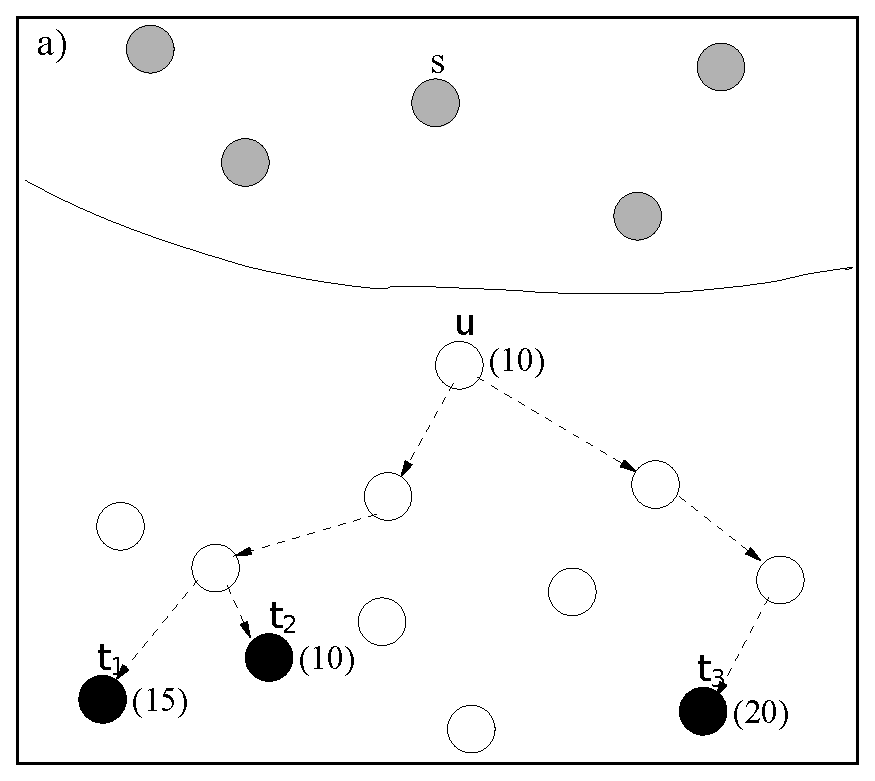
\includegraphics[scale=0.45]{imagens/neigh_teste}}
\subfigure{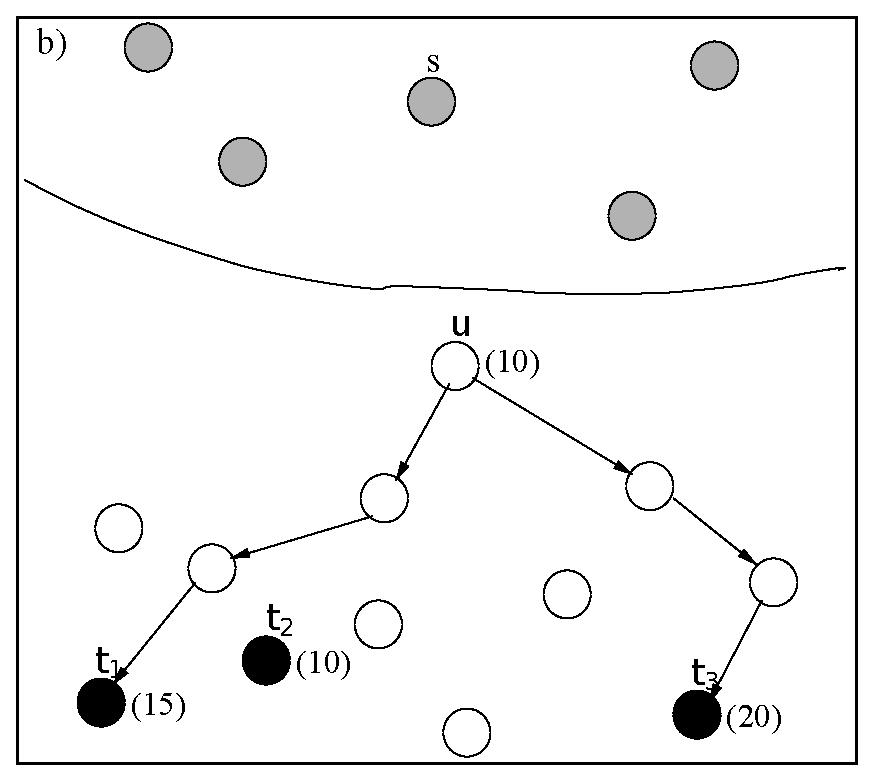
\includegraphics[scale=0.45]{imagens/neigh_color_teste}}
\caption[$\Delta$-neighbourhood of node $u$]{$\Delta$-neighbourhood of node $u$.
%Considering the quantity plotted in the right side of a node $v$ as equal to $dist(s,v,G)$ and considering $dist(u,t_1,G(U)) = 15$, $dist(u,t_2,G(U)) = 12$, $dist(u,t_3,G(U)) = 25$, 
%so $\Delta$-neigh$(u) = \{ t_1,t_3 \}$.
}
\label{fig:delta_neigh}
\end{figure}

Figure \ref{fig:delta_neigh} illustrates the concept of $\Delta$-neighbourhood. The gray nodes represent covered nodes (which are above the division) and the others are 
uncovered nodes (including the black ones which represent terminals in $UT$). Consider $k = 2$ and the quantity plotted in the right side of a node $v$ as equal to $dist(s,v,G)$ and consider 
$dist(u,t_1,G(U)) = 15$, $dist(u,t_2,G(U)) = 12$, $dist(u,t_3,G(U)) = 25$, The dashed paths in 
Figure \ref{fig:delta_neigh}a represent the shortest paths from $u$ to reachable terminals ($t_1$, $t_2$, $t_3$). In Figure \ref{fig:delta_neigh}b, the solid paths represent 
the paths to terminals only that are in $\Delta$-neigh$(u)$, which are $t_1$ and $t_3$.

%\begin{figure}[ht]
%\begin{minipage}[b]{0.46\linewidth}
%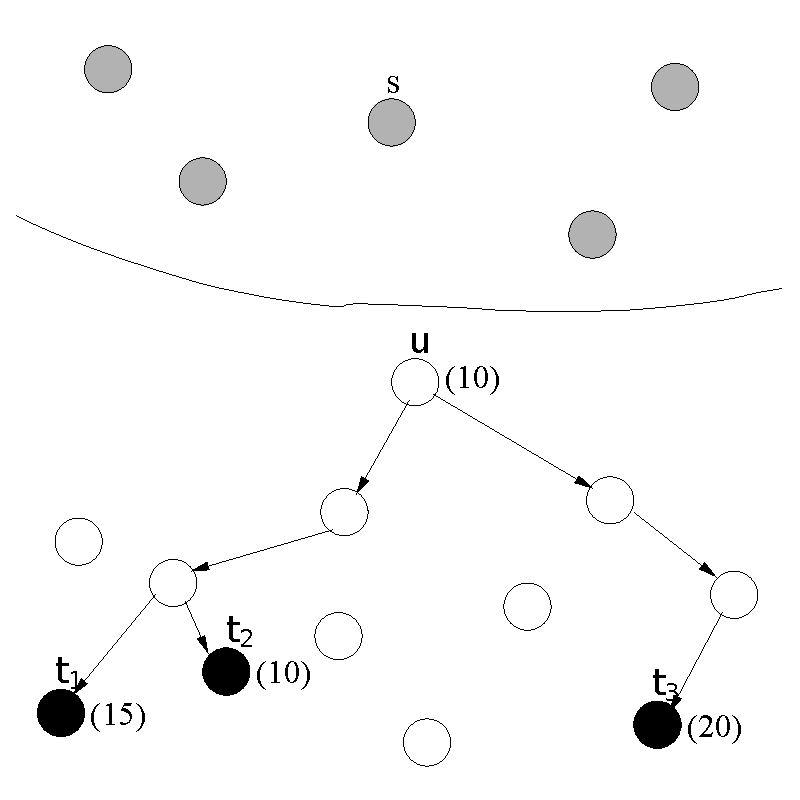
\includegraphics[scale=0.35]{imagens/neigh}
%\caption{PICS spanning factor}
%\label{fig:sigma_interference}
%\end{minipage}
%\hspace{0.3cm}
%\begin{minipage}[b]{0.46\linewidth}
%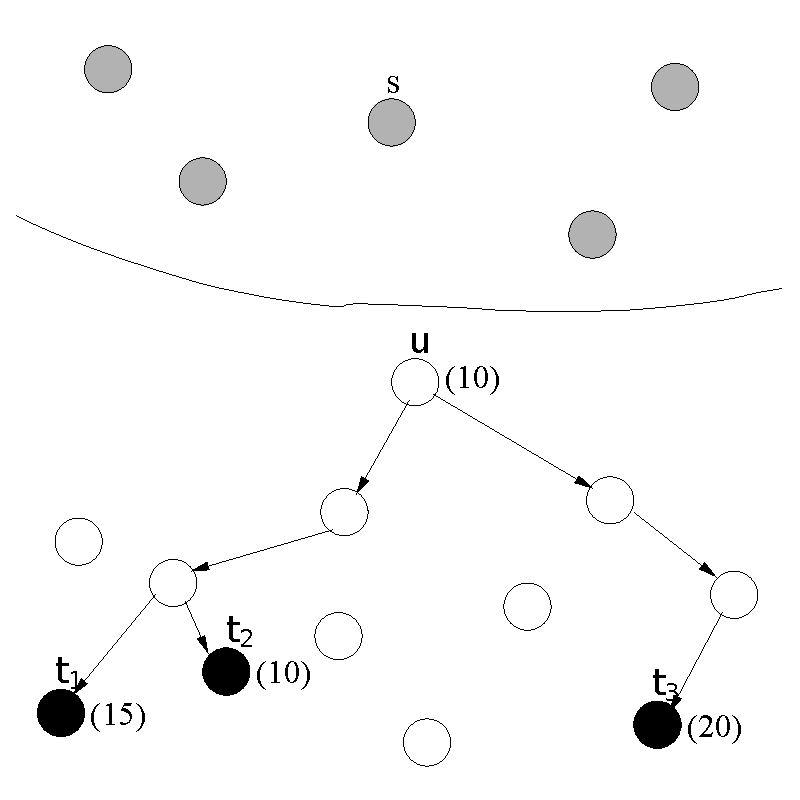
\includegraphics[scale=0.35]{imagens/neigh}
%\caption[]{Maximum PICS spanning factor}
%\label{fig:max_sigma_interference}
%\end{minipage}
%\end{figure}

We denote $SPT(s, S_{leaves}, G)$ a tree rooted at $s$ composed of shortest paths in graph $G$ from $s$ to each of the nodes in $S_{leaves}$.
Finally, for a graph $G$ or a path $P$ we denote $V(G)$ and $E(G)$ as well as $V(P)$ and $E(P)$ the sets of nodes and edges, respectively, of the graph and of
the path.

%informar como derivar o valor de d* (inclusive, isto eh um detalhe da implementaᅵᅵo).

%\subsection{General Description of the Algorithm}
%
%The algorithm has a directed graph $G=(V, E)$ as input and generates a graph $G_{out}=(V_{out}, E_{out})$ as output, which contains a multicast tree. 
%
% where, at the final of this procedure, 
%there is no $\sqrt{k}-bad$ vertex. 
%%Both definitions will be defined later but 
%The idea is to impose a bound on the maximum degree of the arborescences 
%that will be formed in the final of the second phase of the algorithm (whose nodes are uncovered) and at the same time impose a first bound on the degree of the 
%covered nodes at the final of first phase. After the first phase (i.e., after the computation of the $\sqrt k$ \emph{Partition}), there will be an arborescence 
%spanning $s$ and $CT$ with bounded degree. Let us call this arborescence $A_{\sqrt{k}-Par}$.
%%Since the arborescences that will be formed at the final of second phase are formed 

\subsection{First Phase: Computing a $\sqrt{l}$-Partition}

%A \mbox{$\sqrt k$-\emph{partition}}
%is a partition of the elements in $V$ in $m$ partitions $V_1, V_2, ..., V_m$ such that no partition has a \mbox{$\sqrt{k}$-bad} vertex. 
%A vertex $u$ is called a \mbox{$\sqrt{k}$-\emph{bad}} vertex in partition $V_i$ iff $u$ contains more than $\sqrt{k}$ 
%terminals in its $\Delta$-neighborhood. As no partition has a \mbox{$\sqrt{k}$-bad}

In the first phase, the algorithm computes a \mbox{$\sqrt{l}$-\emph{partition}}. 
A \emph{$\sqrt{l}$-partition} divides $V$ into the disjoint and non-empty sets $C$ and $U$, $V = C$ $\cup$ $U$, $C$ $\cap$ $U = \emptyset$, \linebreak
%$U \ne \emptyset$, 
$s \in C$, such that the $\Delta$-neighbourhood of any node in $U$ contains at most $\sqrt{l}$ terminals. A \mbox{$\sqrt{l}$-partition} is computed 
% me parece que esta condicao eh valida nao apenas para UT, mas tambem CT
by eliminating $\sqrt{l}$-\emph{bad} nodes. A node $u$ is called a \mbox{$\sqrt{l}$-\emph{bad}} node if $u$ contains more than $\sqrt{l}$ 
terminals in its \mbox{$\Delta$-neighbourhood}. Procedure \verb|CompPar| (from \cite{Elkin2006}) computes a $\sqrt{l}$-partition.

\begin{figure}[t]
\centering
\subfigure{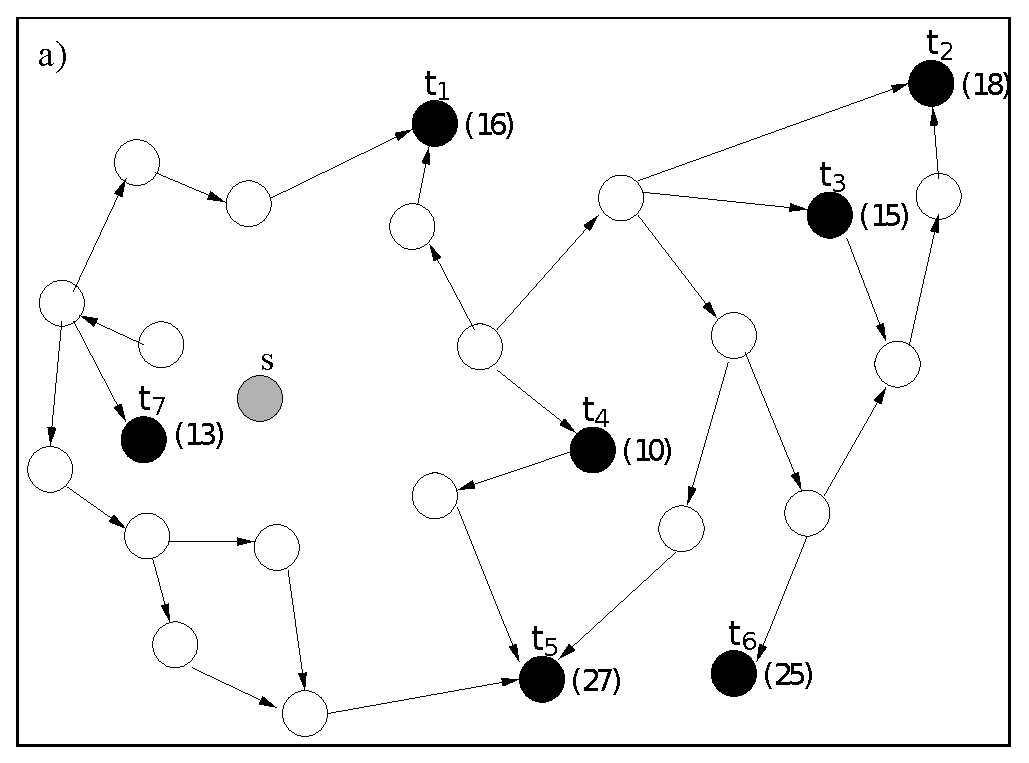
\includegraphics[scale=0.31]{imagens/compPar_teste}}\\
\subfigure{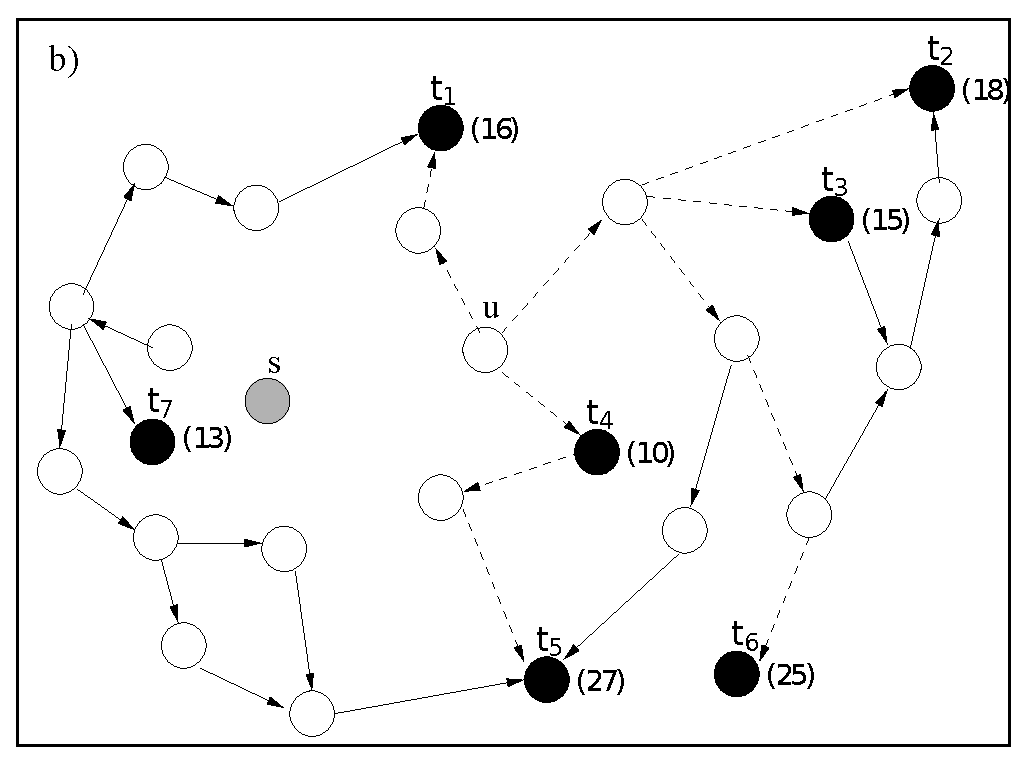
\includegraphics[scale=0.31]{imagens/compPar_bad1_teste}}
\subfigure{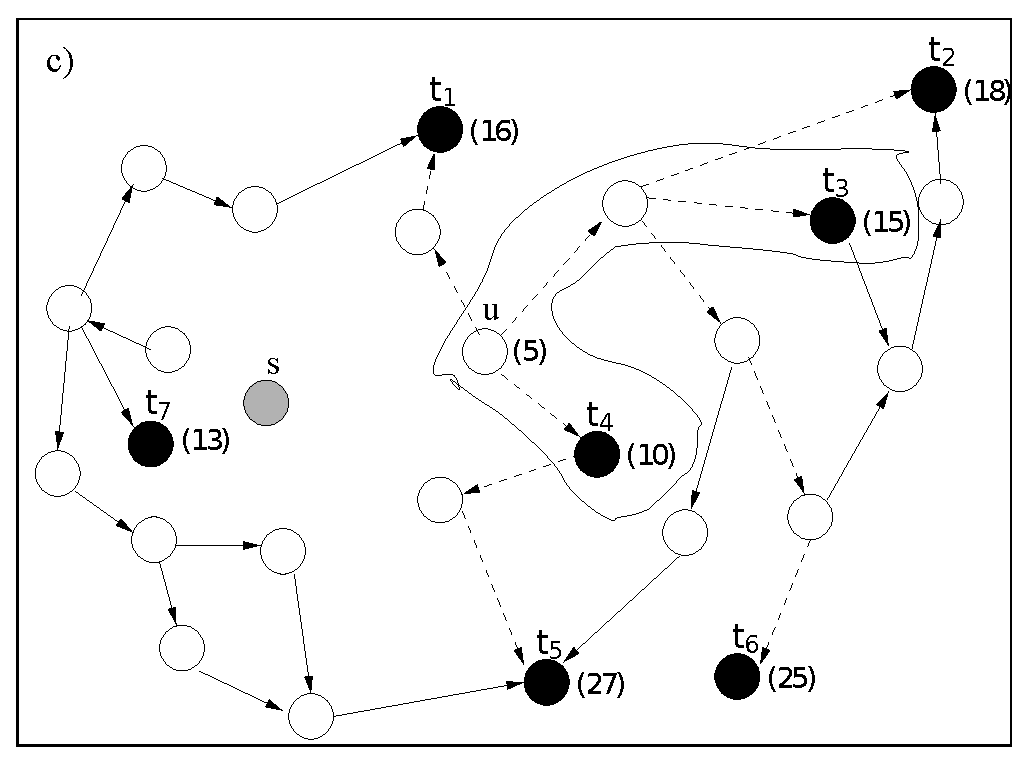
\includegraphics[scale=0.31]{imagens/compPar_tree1_teste}}
\subfigure{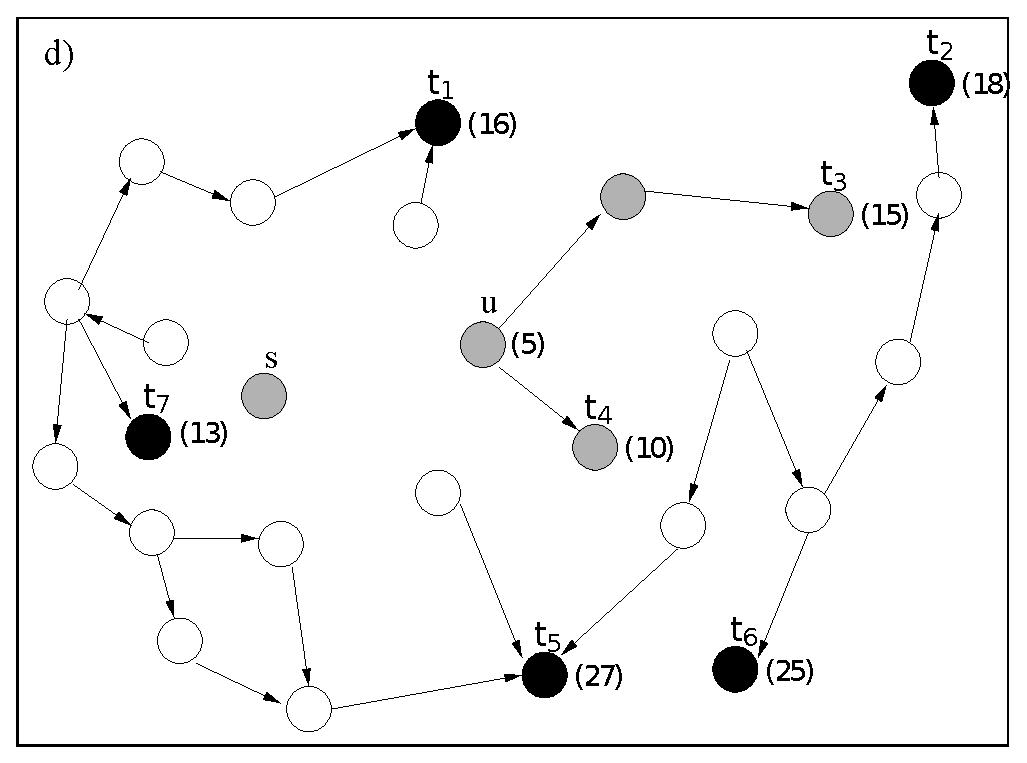
\includegraphics[scale=0.31]{imagens/compPar_cov1_teste}}\\
\subfigure{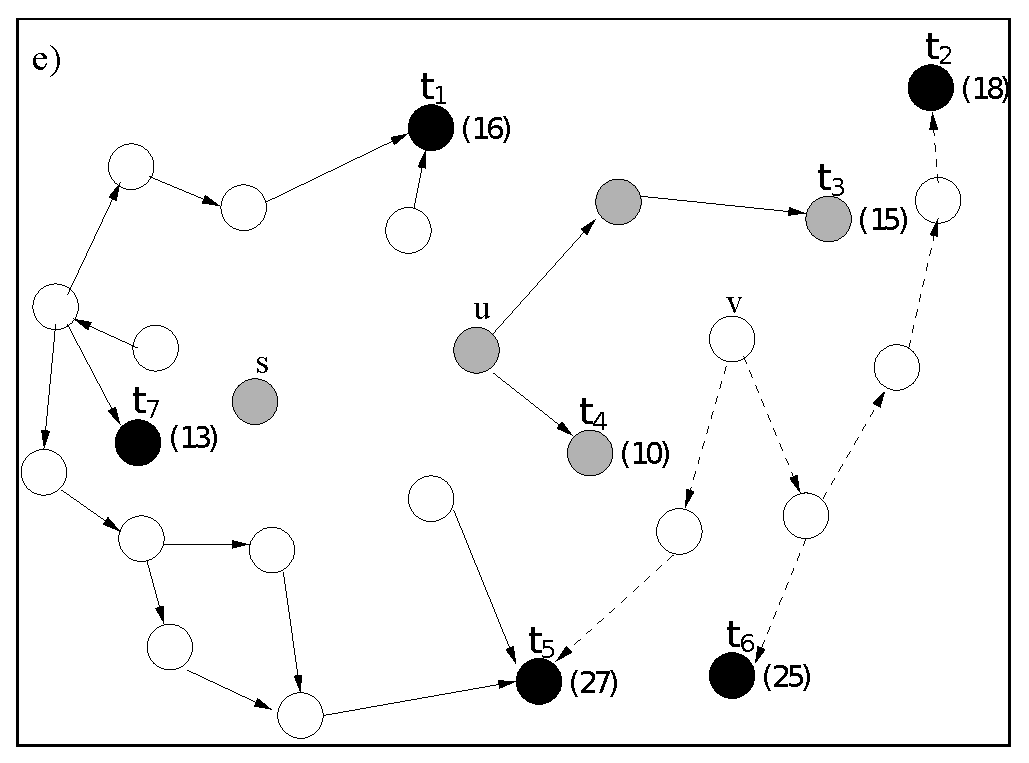
\includegraphics[scale=0.31]{imagens/compPar_bad2_teste}}
\subfigure{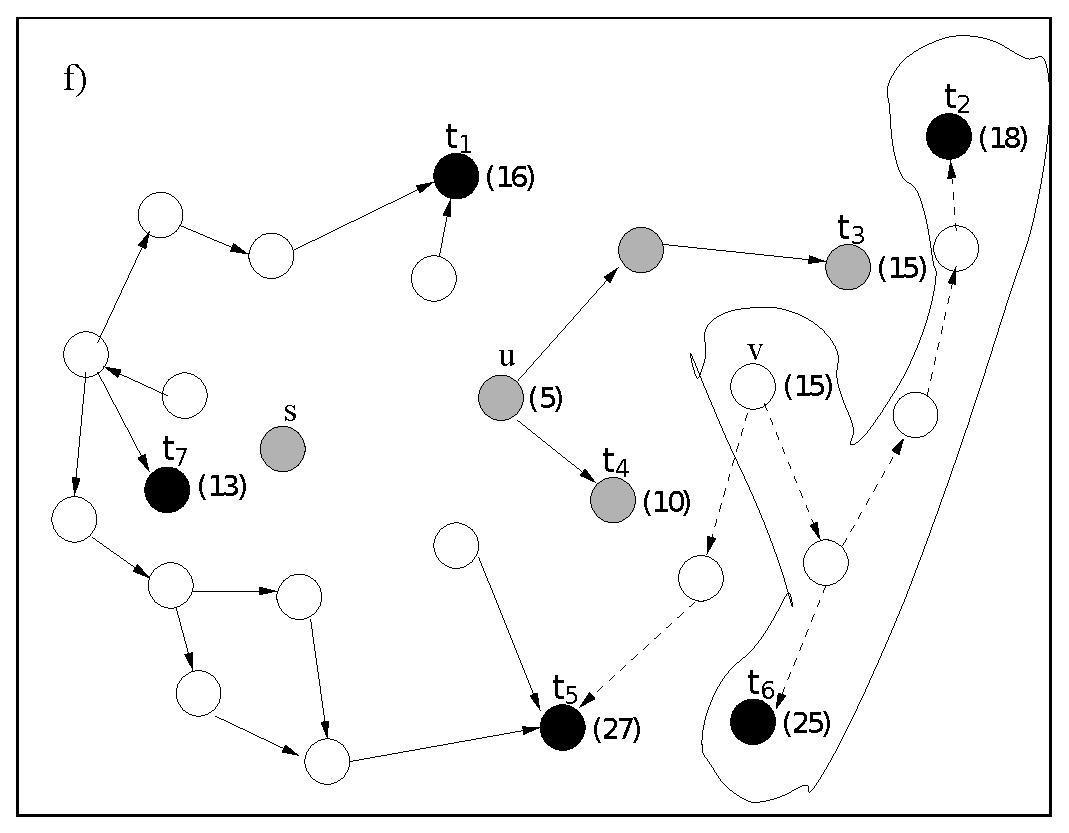
\includegraphics[scale=0.29]{imagens/compPar_tree2_teste}}
\subfigure{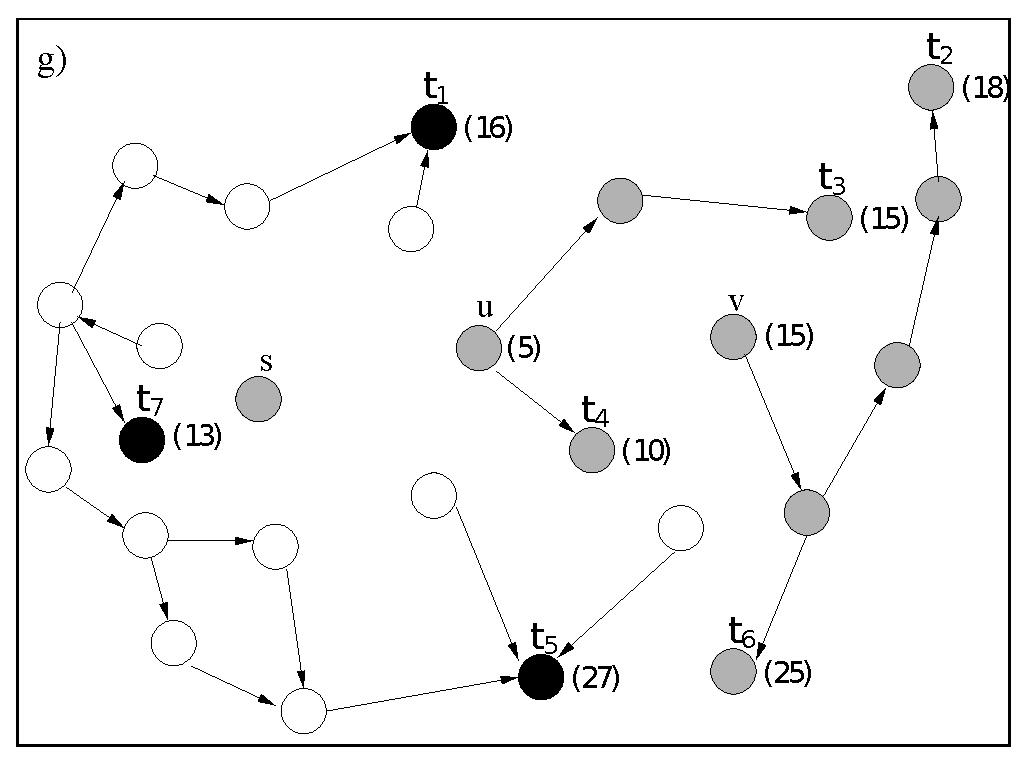
\includegraphics[scale=0.31]{imagens/compPar_cov2_teste}}
\caption[Applying procedure \emph{CompPar}]{Applying procedure \emph{CompPar}.} 
\label{fig:compPar}
\end{figure}

Figure \ref{fig:compPar} illustrates the application of procedure \verb|CompPar|. Gray nodes represent covered nodes and the others are uncovered nodes. 
Consider $k = 2$ and the quantity plotted in the right side of a node $z$ as equal to $dist(s,z,G)$ and consider 
$d(u,t_4,G(u)) = 5$, $d(u,t_3,G(u)) = 10$, $d(u,t_1,G(u)) = 11$, $d(u,t_2,G(u)) = 13$, $d(u,t_6,G(u)) = 20$, $d(u,t_5,G(u)) = 22$, 
$d(v,t_6,G(u)) = 10$, $d(v,t_2,G(u)) = 20$, $d(v,t_5,G(u)) = 24$. 
The dashed paths lead a $\sqrt{l}$-bad node $x$ to $\Delta$-neigh$(x)$ and the circled areas represent the trees removed 
from $G(U)$ and rooted at a previous $\sqrt{l}$-bad node. So, $Roots = \{ u,v \}$.



\begin{procedure}
\label{alg:compute_partition}
$C \gets \lbrace s \rbrace$, $U \gets V \setminus \lbrace s \rbrace$, $Roots \gets \emptyset$\\
\While{$G(U)$ contains a $\sqrt{l}$-bad node $v$}{
  Let $Cl(v)$ be the $\lfloor \sqrt{l} \rfloor$ uncovered terminals closest to $v$ in $G(U)$\\
  Let $T_v$ be a shortest path arborescence leading from $v$ to $Cl(v)$ in $G(U)$\\
  $C \gets C \cup V(T_v)$, $U \gets U \setminus V(T_v)$, $Roots \gets Roots \cup \lbrace v \rbrace$\\
}
Let $H(V_H,E_H)$ be the forest formed by the union of $T_v$, $\forall v \in Roots$\\
Output $(C,U,Roots, H)$
\caption{CompPar(G=(V, E), s, k)} 
\end{procedure}


% where, at the final of this procedure, 
%there is no $\sqrt{k}-bad$ vertex. 
%%Both definitions will be defined later but 
%The idea is to impose a bound on the maximum degree of the arborescences 
%that will be formed in the final of the second phase of the algorithm (whose nodes are uncovered) and at the same time impose a first bound on the degree of the 
%covered nodes at the final of first phase. 

The following lemmas state that \verb|CompPar| computes a correct  
\mbox{$\sqrt{l}$-partition} and that the set $Roots$ has cardinality at most $\sqrt{l} + 2$ (these lemmas are
similar to Claims 2.2 and 2.3 in \cite{Elkin2006} and have analogous proofs - proofs are thus omitted). 
Lemma \ref{lem:proc_comppar} follows from the condition of stopping of the loop of \verb|CompPar| (line 2). 
Lemma \ref{lem:roots_cardinality} follows from the number of terminals removed in each iteration (line 3 of \verb|CompPar|) along with the number of terminals left to be removed in 
the last iteration.

\begin{Lem} 
\label{lem:proc_comppar}
\cite{Elkin2006} The pair $(C, U)$ output by procedure \verb|CompPar| is a \mbox{$\sqrt l$-\emph{partition}}. 
\end{Lem}

\begin{Lem} 
\label{lem:roots_cardinality}
\cite{Elkin2006} $|Roots| \le \sqrt{l} + 2$.
%nao estou convencido deste valor
\end{Lem}

After the computation of a $\sqrt{l}$-partition, we build a directed graph that contains a path from $s$ to each node $t$ in $CT$ that satisfies $k \cdot dist(s,t,G)$ and
which has bounded degree. Let us call this graph $G_{\sqrt{l}-Par}$. It is built as the union of a shortest path from $s$ to each node in $Roots$ and
the $T_v$ trees calculated in line 4 of \verb|CompPar| (represented by forest $H=(V_H, E_H)$, output by \verb|CompPar|). 
This is represented by procedure \verb|CompGraphFirstPh|. %\emph{\ref{alg:compute_arborescence}}.

\begin{procedure}
%$Roots \gets \ref{alg:compute_partition}$\\
$A_{Roots} \gets SPT(s,Roots,G)$\\
%$H(V_H,E_H) \gets \varnothing$\\
%\ForEach{$u \in Roots$}{
%  $H \gets H \cup T_u$\\
%}
%Let $S_{leaves}$ be the set of leaves of all $T_u$, $\forall u \in Roots$\\
$G_{\sqrt{l}-Par} \gets A_{Roots} \cup H(V_H, E_H)$\\
$C \gets V(G_{\sqrt{l}-Par})$, $U \gets V \setminus C$\\
Output $(C,U,G_{\sqrt{l}-Par})$
\caption{CompGraphFirstPh(G, s, Roots, H)} 
\label{alg:compute_arborescence}
\end{procedure}

%Since the arborescences that will be formed at the final of second phase are formed 

%  $A_{\sqrt{k}-Par}$ is computed as follows: compute the shortest path arborescence in $G$ from $s$ to the set $Roots$. Let this arborescence be $A_{roots}$. 
%$A_{\sqrt{k}-Par}$ is formed by the concatenation of $A_{roots}$ to $T_u$, for each $u \in Roots$.

\SetKwInOut{Input}{Input}
\SetKwInOut{Output}{Output}


\begin{Lem}
  \label{lem:roots_size}
%The maximum out-degree of nodes in $G_{\sqrt{k}-Par}$, $D_{max}(G_{\sqrt{k}-Par}), is \linebreak 
The maximum out-degree of nodes in $G_{\sqrt{l}-Par}$ is $\leq 2\sqrt{l} + 2$
%  \begin{proof}
%    $\forall v \in Roots$, $D_{max}(T_v) \leq \sqrt{k}$ (line 5 of \ref{alg:compute_partition}). Let the node $x$ of $H(V_H,E_H)$ be the node with  
%maximum degree and assume its degree as $\sqrt{k}$. When we apply SPT in line 4 of \ref{alg:compute_arborescence}, assume that $y \in V(A_{\sqrt{k}-Par})$ 
%is in the path for $u \in Roots$. If $y = x$ then $y$ is one of the roots in $Roots$ and the proof follows. Otherwise, 
%  \end{proof}
\end{Lem}
\begin{Proof}
The $T_v$ trees computed in line 4 of \verb|CompPar| are disjoint. Each node in these trees has degree at most $\sqrt{l}$,
as each $T_v$ is a shortest path tree to at most $\sqrt{l}$ terminals. $A_{Roots}$ is a shortest path tree from $s$ to the nodes in $Roots$. 
As the cardinality of $Roots$ is at most $\sqrt{l} + 2$ (Lemma \ref{lem:roots_cardinality}), each node in $A_{Roots}$
has degree at most $\sqrt{l} + 2$. As $G_{\sqrt{l}-Par}$ is the union of all these trees, the degree of any of its nodes is limited to $\sqrt{l} + \sqrt{l} + 2 = 2\sqrt{l} + 2$.
\end{Proof}

%\vspace{0.5cm}
%\noindent \textbf{Reducing the problem of cover \emph{UT} to the \emph{Multiple Set-Cover} problem}
%\vspace{0.5cm}

\subsection{Multiple Set-Cover Problem}
\label{sec:msc_definition}

As mentioned before, the MSC problem was stated in \cite{Elkin2003,Elkin2006}. A solution was proposed in \cite{Chekuri2004} based on an approximation algorithm 
for another problem, called \emph{Maximum Coverage with Group Budgets} (MCG). 
%The MSC is a minimization version of an optimization problem where the relative MCG problem consists in a maximization version.

Let $\beta(V_1,V_2,E)$ be a bipartite graph.  A set $S \subseteq V_1$ is called a \emph{set-cover} of $V_2$ if $N(S,\beta) = V_2$. 
The Multiple Set-Cover problem is stated as follows \cite{Elkin2006}:

\vspace{0.3cm}
\noindent \emph{Input}: A bipartite graph $\beta(V_1,V_2,E)$ with \mbox{$|V_1| + |V_2| = n$}. The set $V_1$ is partitioned into a disjoint union of sets 
\mbox{$V_1 = \bigcup_{j=1}^{d}A_j$}. 

\vspace{0.3cm}
\noindent \emph{Output}: A set-cover $S \subset V_1$ of $V_2$ which minimizes $val(S)$, where
\mbox{$val(S) = max\lbrace |S \cap A_i| \rbrace_{i=1}^{d}$}. Figure \ref{fig:msc} illustrates an example.
%\vspace{0.3cm}

\begin{figure}[t]
\centering
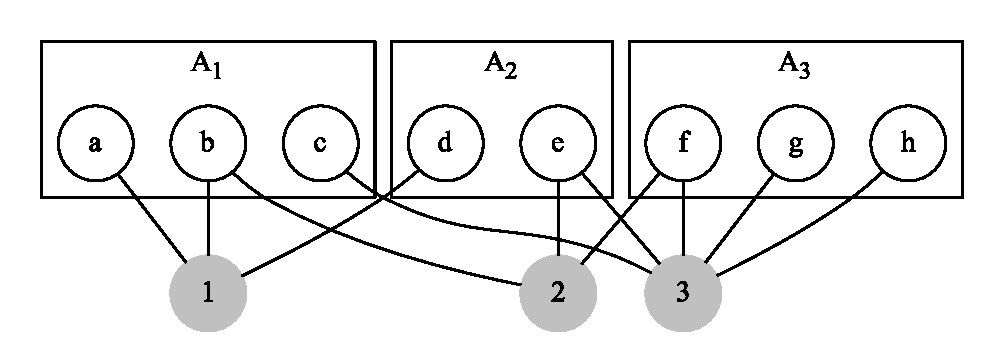
\includegraphics[scale=0.75]{imagens/msc_label}
\caption[Example of MSC]{Example of MSC. Consider $V_1 = \lbrace a,b,c,d,e,f,g,h \rbrace$, $V_2 = \lbrace 1,2,3 \rbrace$ and $A_1$, $A_2$, $A_3$ represent the partitions of $V_1$ ($V_1$ = $A_1 \cup A_2 \cup A_3$). 
The set-covers $S_1 = \lbrace a,e \rbrace$, $S_2 = \lbrace c,d,f \rbrace$ and $S_3 = \lbrace b,f \rbrace$ are examples of optimum solutions, since 
$val(S_1) = val(S_2) = val(S_3) = 1$.}
\label{fig:msc}
\end{figure}

\begin{Theo}
  \label{teorema:fator_aproximacao}
  \cite{Chekuri2004}. The multiple set-cover problem admits a polynomial time greedy $(\log |V_2| + 1)$-approximation algorithm.
\end{Theo}

  In section \ref{sec:solve_msc} we explain how MSC is solved.

\subsection{Second Phase: Covering Nodes in \emph{UT} using an Instance of the \emph{Multiple Set-Cover} Problem}
\label{sec:second-phase}

In the second phase, the remaining nodes in $UT$ become covered. As in \cite{Elkin2006}, we use an instance of the MSC problem
to find paths to cover these nodes while limiting the maximum node degree. 

The second phase is divided into two parts. First,
an instance of MSC is solved to find a specific subset of the covered nodes. In the second
part, we define paths from these covered nodes to the uncovered terminals. 
The union of these paths with $G_{\sqrt{l}-Par}$ generates a graph which contains an arborescence that is a solution
to DSMDStP. 

%Observes that in the construction 
%of $F$ we are concerned with only the degree of the roots of $F$. As we will argue better later, due to the way we define the paths to be considered 
%in the MSC instance and since we have eliminated $\sqrt{k}$-bad nodes (limiting the number of terminals in $UT$ reached through an uncovered node) 
%in the first phase, we only need to care about with the degree of the roots of $F$ that we call \emph{link} nodes (since they are linking covered nodes to 
%uncovered nodes).

The instance of MSC, $\beta=(V_1, V_2, \varepsilon)$, is defined as follows. $V_1$ is composed of \emph{pseudo nodes}. A pseudo node $x_{u, v}$ is created
for each edge $(u, v)$ such that $u$ is a covered node and $v$ is an uncovered node. Formally:
%\begin{displaymath}\label{v1}
\begin{center}
$V_1 = \lbrace x_{u,v} : u \in C, v \in U, (u,v) \in E \rbrace$.
\end{center}
%\end{displaymath}

The set $V_2$ is the set of uncovered terminals, i.e. \mbox{$V_2 = UT$}. The edge set $\varepsilon$ is defined as follows. There is an edge from
pseudo node $x_{u,v}$ to $t \in V_2$ iff the cost of a shortest path from $s$ to $u$ in $G$, plus the cost of $(u, v)$, plus the cost of a shortest path from
$v$ to $t$ in $G(U)$ satisfies the spanner property for $t$. I.e.: 

%\begin{equation}\label{eq:bipartite_edge}
%dist(u,v,G) + dist(v,t,G(U)) \leq \Delta_t.
%\end{equation}
\begin{center}
%\begin{displaymath}\label{eq:bipartite_edge}
$dist(s, u, G) + C(u, v) + dist(v,t,G(U)) \leq k \cdot dist(s,t,G)$.
\end{center}
%\end{displaymath}


Let $A_u = \lbrace x_{u,v} :  v \in N(u, G(U)) \rbrace$. The disjoint partition of $V_1$ that is input for the instance of the MSC problem is 
$V_1 = \bigcup_{u \in C}A_u$. Each partition $A_u$ represents the set of uncovered neighbours of node $u$ in $G(U)$. As there is an algorithm
to MSC that limits \mbox{$A_u$ $\cap$ $S$}, MSC is used to provide a bound to node degree in the final arborescence.

\begin{figure}[t]
\centering
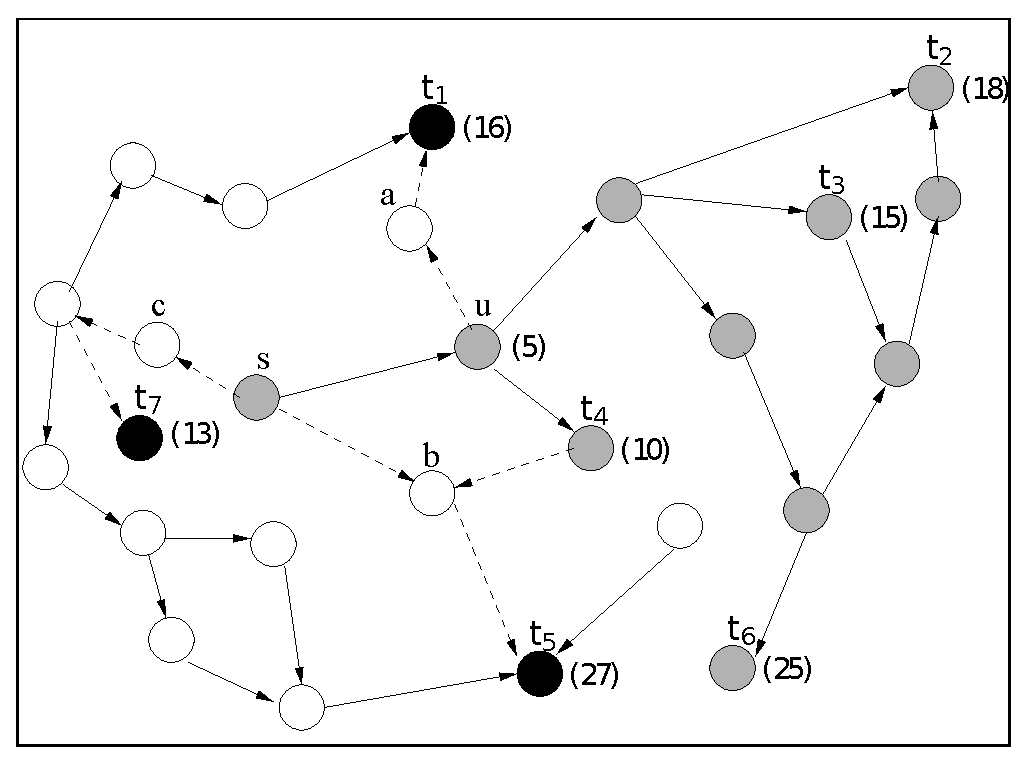
\includegraphics[scale=0.45]{imagens/mscInstance_teste}
\caption[Setting an MSC instance]{Setting an MSC instance.}
\label{fig:mscInstance}
\end{figure}

Figure \ref{fig:mscInstance} illustrates how an MSC instance is set. Gray nodes represent covered nodes and the others are uncovered nodes. 
A dashed path lead a covered node $x$, followed by an uncovered node $y$, to a terminal $t \in UT$ s.t. $dist(s,x,G) + C(x,y) + dist(y,t,G(U)) \le k \cot dist(s,t,G)$. 
We can set $\beta=(V_1, V_2, \varepsilon)$ as $V_1 = \{ X_{u,a}, X_{t_4,b}, X_{s,b}, X_{s,c} \}$, where the disjoint partition of $V_1$ can be represented by the set $\{ \{ X_{u,a} \}, \{ X_{t_4,b} \}, \{ X_{s,b}, X_{s,c} \} \}$, 
$V_2 = \{ t_1, t_5, t_7 \}$, and $\varepsilon = \{ (X_{u,a}, t_1), (X_{t_4,b}, t_5), (X_{s,b}, t_5), (X_{s,c}, t_7) \}$.

%In the optimum DCCMDSttT, $d^* \geq 2$, since the optimum Steiner tree could be a binary tree. We may assume that $d^* \leq k$.

%lemmas

The following lemmas present properties of solutions for such an MSC instance. Their proofs are similar to the 
proofs of Lemmas 3.3 and 3.4 in \cite{Elkin2006}. So we only provide the main idea of the proofs.

\begin{Lem}
  \label{lem:val_solution}
  A  multiple set-cover instance $\beta=(V_1, V_2, \varepsilon)$, as defined above, admits a solution $S^* \subseteq V_1$ such that $val(S^*) \leq d^*$.
\end{Lem}
\begin{Proof}
Let $T^*$ be an optimal solution to an instance of DSMDStP. For any node $t \in UT$, there is a path from $s$ to $t$ in $T^*$. Let $u$ be the last node of this
path that is in $C$ and $v$ the node after $u$ on this path ($v \in U$). So there will be a pseudo node $x_{u, v}$ in $V_1$ and an edge $(x_{u, v}, t) \in \varepsilon$.
As this happens to all nodes in $UT$ and $T^*$ has maximum degree $d^*$, there is a solution $S^*$ for $\beta$ such that
%each pseudo node $x_{u, v}$ will cover at most $d^*$ terminals in $V_2$, as $x_{u, v} \in S^*$ iff $v$ is a child of $u$ in $T^*$. Thus,
for each node $u$ there will be at most $d^*$ pseudo nodes $x_{u,v}$ in the solution $S^*$, as $x_{u, v} \in S^*$ iff $v$ is a child of $u$ in $T^*$. Thus,  
$max_{c \in C}\{|S^* \cap A_c|\}\le d^*$.
\end{Proof}

\begin{Lem}
  \label{lem:max_pseudo_node_degree}
 Let $D$ be a solution to $\beta=(V_1, V_2, \varepsilon)$ with partition $V_1 = \bigcup_{v \in C}A_v$ using Algorithm \ref{alg:greedy} (presented in \cite{Chekuri2004}). 
Then $max_{v \in C}|D \cap A_v| = (\log{l}+1)\cdot d^*$.
\end{Lem}
\begin{Proof}
As $d^*$ is greater than or equal to $val(S^*)$ for an optimal solution $S^*$ of $\beta$ and $|V_2| \le l$, this lemma is a direct application of Theorem \ref{teorema:fator_aproximacao}.
\end{Proof}

In order to build the final solution to DSMDStP, we first add to $G_{\sqrt{l}-Par}$ a set of shortest 
paths from covered nodes to terminals in $UT$ and compute a shortest path arborescence over the resulting graph.
We use $D$ to choose the covered nodes. The complete algorithm to DSMDStP is given in the section \ref{sec:complete_algorithm}. 

\subsection{The Complete Algorithm}
\label{sec:complete_algorithm}

Algorithm \ref{alg:approximation} represents the complete algorithm. Lines 1-2 represent the first phase.
After computing a $\sqrt{l}$-partition (line 1), graph $G_{\sqrt{l}-Par}$ is computed (line 2).
%Lines 4-13 correspond to the second phase of the algorithm. In lines 4-5 represent the instance of the MSC problem (first part of the second phase).
Lines 3-4 correspond to the first part of the second phase of the algorithm, i.e. the application of the algorithm in \cite{Chekuri2004} to an instance of the MSC problem
(as described in Section \ref{sec:second-phase}). 
The output of this algorithm is the set $D$, whose elements cover $V_2$. 
Lines 5-12 correspond to the second part of the second phase, when the arborescence that is output of the algorithm is built.

In lines 5-10 the digraph $\varGamma(V_{\varGamma},E_{\varGamma})$ is built. For each uncovered node $t$ in $UT$, we choose a node $x_{u, v}$ in $D$
such that there is an edge $(x_{u, v}, t) \in \varepsilon$ and $C(u, v) + dist(v,t,G(U))$ is minimum. The set $V_\varGamma$ is composed of the nodes $u$ and the set of nodes on a shortest path
from $v$ to $t$. The set $E_\varGamma$ contains the edges in these paths and edges $(u, v)$.

In line 11, we build the graph $G_f$, which is the union of graphs $G_{\sqrt{l}-Par}$ and $\varGamma$. 
We finally compute the arborescence $\mathcal{A}_f$ that is the output of the algorithm. $\mathcal{A}_f$ is a shortest
path tree in $G_f$ rooted at $s$, containing shortest paths from $s$ to the terminals. 

\SetKwInOut{Input}{Input}
\SetKwInOut{Output}{Output}
%\SetKwComment{coment}{\{}{\}}

\begin{algorithm}
\Input{$G=(V, E)$, $s \in V$, $T \subset V$, $k$}
\Output{$\mathcal{A}_f =(V_{\mathcal{A}_f}, E_{\mathcal{A}_f})$}
\BlankLine
  %$C \gets s$, $U \gets V \setminus \lbrace s \rbrace$\\
  $(C, U, Roots, H) \gets$ \verb|CompPar|($G, s, k$) \\ %\coment{Run Procedure \emph{\ref{alg:compute_partition}} to compute the $\sqrt{k}$ Partition}
  $(C, U, G_{\sqrt{l}-Par})\gets\verb|CompGraphFirstPh|(G,s,Roots,H)$ \\	
  Build the MSC instance $\beta = (V_1, V_2, \varepsilon)$ as in Section \ref{sec:second-phase} \\
  $D \gets $ Apply approximation algorithm \cite{Chekuri2004} on $\beta$\\
  $\varGamma(V_{\varGamma},E_{\varGamma}), V_{\varGamma} \gets \emptyset, E_{\varGamma} \gets \emptyset$\\
%  \ForEach{$x_{u,v} \in D$}{
%    $S_{ter} \gets \lbrace t : t \in V_2 \wedge (x_{u,v},t) \in \varepsilon \rbrace$ \\
%    \ForEach{$t \in S_{ter}$}{
%           $s \gets sp(u,t,G(U))$ \\
%           $V_{\varGamma} \gets V_{\varGamma} \cup V(s)$ \\ 
%    	  $E_{\varGamma} \gets E_{\varGamma} \cup E(s)$ \\
%	}
%  }
  \ForEach{$t \in V_2$}{
    Choose $x_{u, v} \in D$ : $(x_{u, v}, t) \in \varepsilon$ and $C(u, v) + dist(v,t,G(U))$ is minimum \\
    $s \gets sp(v, t, G(U))$ \\
    $V_{\varGamma} \gets V_{\varGamma} \cup \{u\} \cup V(s)$ \\ %, \forall q, q \in S_{ter}$\\% \wedge q \notin V_{\varGamma}$ \\
    $E_{\varGamma} \gets E_{\varGamma} \cup \{(u, v)\} \cup E(s)$ \\ %, \forall q, q \in S_{ter}$\\% \wedge q \notin V_{\varGamma}$ \\

 }
  $G_f \gets G_{\sqrt{l}-Par} \cup \varGamma(V_\varGamma,E_\varGamma)$ \\
  $\mathcal{A}_f \gets SPT(s, T, G_f)$

%  $\forall x_{u,v} \in D$, add $u$ to $S_{PS}$\\
%  %PS - possible sources
%  $F(V_F,E_F) \gets$ Apply Prim's algorithm to $\varGamma(V_{\varGamma},E_{\varGamma})$ considering the sources $S_{PS}$ and destinations $UT$\\
%  $A_{final} \gets A_{\sqrt{k}-Par} \cup F(V_F,E_F)$

\caption{Approximation Algorithm to \mbox{DSMDStP}} 
\label{alg:approximation}
\end{algorithm}


\begin{Lem}
  \label{lem:max_degree}
  The maximum out-degree of nodes in $G_f$ is $\leq 2\sqrt{l} + 2 + O(\log l) \cdot d^*$.
\end{Lem}
  \begin{Proof}
The algorithm adds nodes to $G_f$ in the first and second phases of the algorithm. After the first phase, each node in $G_f$ has
maximum out-degree $2\sqrt{l} + 2$ (Lemma \ref{lem:roots_size}). In the second phase, new nodes are added to $G_f$ and the out-degree of
nodes already in $G_f$ might increase. The new added nodes have maximum degree $\sqrt{l}$, as, in this phase, there are no more $\sqrt{l}$-bad
nodes. The nodes already in $G_f$ that might have their degrees increased are those nodes $u$ for which there is a pseudo node $x_{u, v}$ in $D$. 
However, from Lemma \ref{lem:max_pseudo_node_degree}, the out-degree of these nodes might be increased by at most $O(\log l) \cdot d^*$. 
Thus, the maximum out-degree of any node is $2\sqrt{l} + 2 + O(\log l) \cdot d^*$.
  \end{Proof}

\begin{Lem}
  \label{lem:cost_guaranteed}
$\forall t \in T$, $dist(s,t,G_f) \leq k \cdot ( dist(s,t,G) + dist(s,t_{max},G))$, 
where $t_{max} \in \{t' | 
(t' \in T) \land (\forall t'' \in T : dist(s,t'',G) \le dist(s,t',G))\}$.
\end{Lem}
  \begin{Proof}
If $t$ is covered in the first phase, 
$dist(s, t, G_f) \le k \cdot dist(s,t,G)$ by construction: a tree rooted at a (previously) $\sqrt{l}$-bad node $u$ contains paths from $u$ to terminals $t$ such that 
$dist(s, u, G) + dist(u, t, G) \le k \cdot dist(s,t,G)$. In particular, all nodes $v$ (terminals or not) that are covered in the first phase, are in a path
from $s$ to a terminal $t$ with cost less than or equal to $k \cdot dist(s,t,G)$, which is $\le k \cdot dist(s,t_{max},G)$. 

For the terminals $t$ that are only covered in the second phase (as in the proof of Lemma \ref{lem:val_solution}, for each $t$, there is 
a path between $s$ and $t$), observe that
a pseudo node $x_{u, v}$ and an edge $(x_{u, v}, t)$ are inserted in the input graph to the MSC instance 
if $dist(s, u, G)+C(u,v)+dist(v,t,G(U)) \leq k \cdot dist(s,t,G)$. Thus, in particular, $C(u,v)+dist(v,t,G(U)) \le k \cdot dist(s,t,G)$.
As $dist(s, u, G) \le k \cdot dist(s,t_{max},G)$, we have
$dist(s,t,G_f) \leq k \cdot (dist(s,t,G) + \cdot dist(s,t_{max},G))$.
  \end{Proof}

By Lemma \ref{lem:cost_guaranteed}, the algorithm can violate the spanner property for some terminals. Observe, however, that this might only happen
to terminals covered in the second phase. Terminals covered in the first phase have their spanner constraint satisfied.

\begin{Theo}
  \label{teorema:final_theorem}
  The approximation algorithm generates an arborescence $\mathcal{A}_f$ with bounded out-degree $2\sqrt{k} + 2 + O(\log l) \cdot d^*$ and that 
has paths from $s$ to each terminal $t \in T$ with cost less than or equal to $k \cdot ( dist(s,t,G) + dist(s,t_{max},G))$, 
where $t_{max} \in \{t' | 
(t' \in T) \land (\forall t'' \in T : dist(s,t'',G) \le dist(s,t',G))\}$.
\end{Theo}
  \begin{Proof}
The $\mathcal{A}_f$ tree is generated by computing minimum cost paths in $G_f$ from $s$ to each $t \in T$. The theorem follows from the fact that
all nodes in $G_f$ have out-degree $\le 2\sqrt{l} + 2 + O(\log l) \cdot d^*$ (Lemma \ref{lem:max_degree}) and that $G_f$ contains paths from $s$ to each $t \in T$ 
with costs $\le k \cdot ( dist(s,t,G) + dist(s,t_{max},G))$ (Lemma \ref{lem:cost_guaranteed}).
  \end{Proof}

%In order to evaluate the bound on node-degree of the algorithm, it was proved that there is no sublogarithmic approximation to the 
%Steiner version of the \emph{Minimum Degree Spanning Tree} (MDS) in digraphs \cite{Fraigniaud2001}, which is a restriction of DSMDStP.

\subsection{Complexity}

The \verb|CompPar| procedure has its complexity bounded by $(\sqrt{|T|} + 2)O(|V|^3)$ due to the number of loop iterations (Lemma \ref{lem:roots_cardinality}) and 
the complexity of building a shortest path tree (SPT) for the $\sqrt{l}$-bad node candidates, using Dijkstra's algorithm \cite{Cormen2009}. The complexity of the procedure \verb|CompGraphFirstPh| 
is bounded by the running time of building SPT, so it is bounded by $O(|V|^2)$.

The complexity of building the MSC instance (line 3) is related to the complexity of composing the sets $V_1$ and $\varepsilon$. 
The former is bounded by $O(|V|^2)$ 
where the latter is bounded by the running time of all-pair-shortest paths (APSP) algorithm, which is $O(|V|^3)$ \cite{Cormen2009}.

We assume the algorithm described in \cite{Chekuri2004} (Algorithm \ref{alg:msc}) for solving instances of the MSC problem (line 4).
This algorithm is based on an algorithm (Algorithm \ref{alg:greedy}) for another problem, called MCG. The algorithm to MCG depends
on calls to an oracle, which have, in our case, $O(|V|^2|T|)$ running time. The complexity of MCG will
thus be $O(|V|^3|T|^2)$. As the MSC algorithm 
consists in iteratively applying the MCG algorithm, the running time of line 4 is $O((\log{|T|})(|V|^3|T|^2)$
(refer to \cite{Chekuri2004} or Section \ref{sec:solve_msc} for the details).

Using the result of the APSP algorithm run for building the MSC instance, the complexity of a single run of 
lines 7-10 is bounded to $O(|V|^2)$. As the number of iterations of the loop in lines 6-10 is bounded by the size of $D$,
the complexity of lines 6-10 is $|T|O(|V|^2)$.

So, the complexity of Algorithm \ref{alg:approximation} is bounded by the complexity of solving MSC, 
which is $O((\log{|T|})(|V|^3|T|^2)$.
%It is easy to verify that the algorithm has polynomial execution time, as it is basically composed of operations on sets,
%computation of minimum cost paths and on the algorithm in \cite{Chekuri2004}, which is polynomial (Theorem \ref{teorema:fator_aproximacao}).
%\end{spacing}

\section{Heuristic for the DSMDStP}
\label{sec:heuristic}
%\begin{spacing}{1.5}
%\parskip=6pt

In this section we describe a heuristic called \emph{Sliced and Iterative MSC} (SIM) for the DSMDStP. In this heuristic, the 
cost of the paths from $s$ to each terminal $t$ in the final arborescence is less than or equal to $k \cdot (\lfloor\sqrt{|T|}\rfloor+2) \cdot dist(s,t,G)$.
% (in the algorithm of Section \ref{sec:algorithm}, the costs of these paths are limited to $\Delta_t + \Delta_{max}$). 

\subsection{Algorithm}
\label{sec:heuristic-description}

As the name says, the heuristic is iterative. The terminals are iteratively covered in ascending order of the costs of the shortest paths  
from the source node to each of them in $G$. At each iteration, the heuristic covers the next uncovered $\lfloor\sqrt{l}\rfloor$ terminals in this order,
until there are no more uncovered nodes. 
Instead of using MSC only once to find paths to all the remaining uncovered terminals (as in the approximation algorithm), we use MSC at each iteration to cover the 
next uncovered $\lfloor\sqrt{l}\rfloor$ terminals in order. The set of these terminals will be referred to as $Next^{\sqrt{l}}_{ter}$. 
%The term \emph{Sliced} is in the name of the heuristic since we cover a subset (\emph{slice}) of the terminal at each turn.

In order to build an MSC instance, we create pseudo nodes $x_{u, v}$ as in Section \ref{sec:second-phase}. However, in order to
try to decrease the out-degree of nodes, we mark nodes $u$ that have already been part of a solution of an MSC instance (in a
previous iteration).
We try to create paths to uncovered terminals from unmarked nodes. However, when necessary, we use marked nodes. The set of
marked nodes is called $Marked$.


%  Formally, considers $OL_{ter}$ the ordered list of $UT$ by the respective cost parameters. Let $t_i$ be the terminal of $OL_{ter}$ with the \emph{i-th} lowest cost parameter $\Delta_i$. 
%Let $Next^{\sqrt{k}}_{ter}$ be the next $\sqrt{k}$ terminals of $OL_{ter}$. Considers the bipartite graph $B_{C,U}(V'_1,V'_2,\varepsilon')$ defined as follows:

\SetKwInOut{Input}{Input}
\SetKwInOut{Output}{Output}

\begin{algorithm}[t]
\Input{$G=(V, E)$, $s \in V$, $T \subset V$, $k$}
%$k \cdot dist(s,t,G), \forall t \in T$}
\Output{$\mathcal{A}_f=(V_{\mathcal{A}_f}, E_{\mathcal{A}_f})$}
\BlankLine
%  Order T by $\Delta_{i}$ to form $OL_{ter}$. Let $t_i$ be the terminal of $OL_{ter}$ with the \emph{i-th} lowest cost bound $\Delta_i$\\
  %Let $Next_{ter}^{\sqrt{k}}$ be the next $\sqrt{k}$ terminals of $OL_{ter}$ \\
  $C \gets \{s\}$, $U \gets V \setminus \lbrace s \rbrace$, $Marked \gets \emptyset$, $l \gets |T|$ \\
  \While{$UT \neq \emptyset$}{
    Set $V_1, V_2$ and $\varepsilon$ using the current values of $C$, $U$, $Marked$ and $Next^{\sqrt{l}}_{ter}$ 
	(See Section \ref{sec:heuristic-description})\\
%    Set $V'_1$ disregarding the nodes $x_{u,v}$ where $u$ is marked\\
    \ForEach{$t : t \in V_2$ and $\nexists$ edge $(x,t) \in \varepsilon$ for any $x$}{
      Let $x_{u, v}$ be a pseudo node such that: \linebreak
	\hspace*{0.4cm} $u \in Marked$, \linebreak
	\hspace*{0.4cm} $u$ has the smallest out-degree and 
	\hspace*{0.4cm} $C(u,v) + dist(v,t,G(U)) \leq k \cdot dist(s,t,G)$\\
      $V_1$ $\gets$ $V_1 \cup \{x_{u,v}\}$,  $\varepsilon \gets \varepsilon \cup \{(x_{u,v},t)\}$ \\
    }
    $D \gets $ Apply approximation algorithm \ref{alg:msc} on $\beta(V_1, V_2, \varepsilon)$\\
    $\varGamma(V_{\varGamma},E_{\varGamma}) \gets \emptyset$\\
  \ForEach{$t \in V_2$}{
    Choose a node $x_{u, v} \in D: (x_{u, v},t) \in \varepsilon$ and $C(u, v) + dist(v,t,G(U))$ is \linebreak
	\hspace*{0.5cm} minimum\\
    $Marked \gets Marked$ $\cup$ $\{u\}$ \{ for which $x_{(u,v)}$ was chosen in the last line\} \\
    $s \gets sp(v, t, G(U))$ \\
    $V_{\varGamma} \gets V_{\varGamma} \cup \{u\} \cup V(s)$ \\ %, \forall q, q \in S_{ter}$\\% \wedge q \notin V_{\varGamma}$ \\
    $E_{\varGamma} \gets E_{\varGamma} \cup \{(u, v)\} \cup E(s)$ \\ %, \forall q, q \in S_{ter}$\\% \wedge q \notin V_{\varGamma}$ \\
  }
%    \ForEach{$x_{u,v} \in D'$}{
%      $S_{ter} \gets$ $\{ t : t \in V'_2 \wedge (x_{u,v},t) \in \varepsilon' \rbrace$ \\
%      $V_{\varGamma} \gets V_{\varGamma} \cup \lbrace u \rbrace \cup V(sp(v,q, G(U))), \forall q, q \in S_{ter}$\\% \wedge q \notin V_{\varGamma}$ \\
%      $E_{\varGamma} \gets E_{\varGamma} \cup \lbrace (u,v) \rbrace \cup E(SP_{G(U)}(v,q)), \forall q, q \in S_{ter}$\\% \wedge q \notin V_{\varGamma}$ \\
%    }
%    $\forall x_{u,v} \in D'$, add $u$ to $S_{PS}$\\
%   %PS - possible sources
%    $F(V_F,E_F) \gets$ Apply Prim's algorithm to $\varGamma(V_{\varGamma},E_{\varGamma})$ considering the sources $S_{PS}$ and destinations $V'_2$\\
%    $S_{cov-ter} \gets UT \cap V_F$\\
%    $OL_{ter} \gets OL_{ter} \setminus S_{cov-ter}$\\
    $C \gets C \cup V_\varGamma$, $U \gets U \setminus V_\Gamma$\\
    %$U \gets U \setminus V_F$\\
    $\mathcal{A}_f \gets \mathcal{A}_f \cup \Gamma(V_\Gamma,E_\Gamma)$
  }
\caption{SIM - \emph{Sliced and Iterative MSC}} 
\label{alg:sim}
\end{algorithm}  

SIM is represented as Algorithm \ref{alg:sim}. In line 1, the sets $C$, $U$, $Marked$ and $l$ are initialized ($C$, $U$ and $l$ are used as in Section \ref{sec:algorithm}). 

The main loop of SIM (lines 2-16) represents the iterations. In lines 3-6, we define the values of $V_1, V_2$ and $\varepsilon$ to build an instance
$\beta = (V_1, V_2, \varepsilon)$ of MSC. The sets $V_1$, $V_2$ and $\varepsilon$ are initialized as follows:
\begin{align*}
%\begin{split}
%V_1^j = \lbrace x_{v,u} | v \in C_j, u \in U_j, (v,u) \in \varepsilon_j \rbrace.
%V'_1 = \lbrace x_{u,v} | u \in C, v \in Next_{ter}^{\sqrt k}, (u,v) \in E \rbrace.
V_1& = \lbrace x_{u,v} : u \in (C \setminus Marked), v \in U, (u,v) \in E \rbrace,\\ 
V_2& = Next^{\sqrt{l}}_{ter},\\ 
\varepsilon& = \{(x_{u,v}, t) : x_{u,v} \in V_1 \land t \in Next^{\sqrt{l}}_{ter} \land C(u,v) + dist(v,t, G(U)) \leq k \cdot dist(s,t,G)\}.
%\end{split}
\end{align*}
%\begin{center}
%$\varepsilon = \{(x_{u,v}, t) : x_{u,v} \in V_1$ $\land$ $t \in Next^{\sqrt{l}}_{ter}$ $\land$ $C(u,v) + dist(v,t, G(U)) \leq k \cdot sp(s,t,G)$\}.
%\end{center}

First, we only consider unmarked nodes in $C$, as explained before. But, in doing so there is the possibility of there being nodes in $V_2$ that cannot
be covered (for example, if the only path from a covered to an uncovered node that has cost $\le k \cdot dist(s,t,G)$ for some $t$ has, as its last covered node, an already marked one).
So, when needed, we include in $V_1$ pseudo nodes $x_{u, v}$ for marked nodes $u$. In these cases, we include a node $x_{u, v}$ such that $u$ is a marked node 
with the smallest out-degree and
the sum of the cost of edge $(u, v)$ and of a shortest path from $v$ to $t$ in $G(U)$ is $\le k \cdot dist(s,t,G)$ (lines 4-6). 
We thus apply the approximation algorithm \ref{alg:msc} to $\beta (V_1, V_2, \varepsilon)$, using $V_1 = \bigcup_{u \in C}A_u$ as the partition,
where $A_u=\{x_{u,v} : \exists v \in V$ such that $x_{u,v} \in V_1\}$ (line 7). $D$ is the output of this algorithm.

In lines 8-14 we choose paths from covered nodes to the terminals in $Next^{\sqrt{l}}_{ter}$. For each node $t \in V_2$ we choose
a pseudo node $x_{u, v}$ in $D$ such that there is a path from $u$ to $t$ with cost $\le k \cdot dist(s,t,G)$. These are the nodes $x_{u, v}$ for which
there is an edge $(x_{u, v}, t) \in \varepsilon$. We choose the pseudo node $x_{u, v}$ for which the path composed of the edge $(u, v)$ and
a shortest path from $v$ to $t$ has the smallest cost (line 10). We thus mark node $u$ (line 11) and store this path in $\varGamma$ (lines 12-14).

In line 15, the set of covered ($C$) and uncovered ($U$) nodes are updated. The nodes in $V(\varGamma)$ become covered. Finally, 
the nodes and edges of $\varGamma$ are added to the arborescence $\mathcal{A}_f$ (line 16). 

At the end of the last iteration, $\mathcal{A}_f$ contains the final arborescence.

%In lines 4-5, we set the MSC instance $\beta' = (V'_1, V'_2, \varepsilon')$ but when setting $V'_1$ we disregard $x_{u,v}$ if $u$ was marked before. 
%The marked nodes represent the nodes $y$ where $x_{y,z}$ was chosen to be part of $V'_1$ in some instance $\beta'$ given as input to the MSC. 
%Once a node becomes marked it remains marked until the end. $\forall x_{u,v} \in V'_1$, let us call the node $u$ \emph{pseudo node root}. 

\begin{Lem}
  \label{lem:terminals_covered}
  Let $\mathcal{A}_f$ be output by SIM. $\forall t \in T$, there is a path from $s$ to $t$ in $\mathcal{A}_f$.
\end{Lem}
  \begin{Proof}
    Let $T^*$ be an optimal solution to an instance of DSMDStP. For any node $t \in UT$, there is a path from $s$ to $t$ in $T^*$. Similar to the proof of Lemma \ref{lem:val_solution}, 
let $u$ be the last node of this path that is in $C$ and $v$ the node after $u$ on this path ($v \in U$). Irrespective the iteration which $t$ is added to $Next^{\sqrt{l}}_{ter}$, 
there will be a pseudo node $x_{u, v}$ in $V_1$ and an edge $(x_{u, v}, t) \in \varepsilon$. So, after applying approximation algorithm \ref{alg:sim} on $\beta(V_1, V_2, \varepsilon)$ (line 7), 
we know there will be at least one path leading from a covered node $u$ to $t$, and one of these paths is chosen by SIM to be part of $\mathcal{A}_f$ (line 12), concluding the proof.
  \end{Proof}


%nao foi revisado por Blanche
\begin{Lem}
  \label{lem:number_iterations}
  The number of SIM's iterations is bounded by $\lfloor\sqrt{l}\rfloor + 2$.
\end{Lem}
  \begin{Proof}
%Now consider the number of terminals $l$. If $l$ is a perfect square, it is easy to see that all terminals will be covered in $\sqrt{l}$ iterations (since $\lfloor\sqrt{l}\rfloor$ terminals = $\sqrt{l}$ terminals). 
%If $l$ is not a perfect square, 
%we have to divide the total amount of $l$ in two factors, $F_1$ (the number of terminals covered in each iteration, which means $F_1 = \lfloor\sqrt{l}\rfloor$) and 
%$F_2$ (the number of iterations) such that $l = F_1 \cdot F_2$. Actually, $F_2$  will be a bound in the number of iterations. 

Consider the number of terminals $l$. If $l$ is a perfect square, it is easy to see that all terminals will be covered in $\sqrt{l}$ iterations (since $\lfloor\sqrt{l}\rfloor$ terminals = $\sqrt{l}$ terminals). 
Now let us examine the case where $l$ is not a perfect square.

Let $\sqrt{l} = \lfloor\sqrt{l}\rfloor + \mathcal{F}$, where $\mathcal{F} \in ]0,1[$. Then $l = (\lfloor\sqrt{l}\rfloor + \mathcal{F}) \cdot (\lfloor\sqrt{l}\rfloor + \mathcal{F})$. So:

\begin{align*}
%l& = \left(\lfloor\sqrt{l}\rfloor \cdot \lfloor\sqrt{l}\rfloor\right) + (\lfloor\sqrt{l}\rfloor \cdot \mathcal{F}) + (\lfloor\sqrt{l}\rfloor \cdot \mathcal{F}) + (\mathcal{F} \cdot \mathcal{F})\\
%l& = (\lfloor\sqrt{l}\rfloor \cdot \lfloor\sqrt{l}\rfloor) + [\lfloor\sqrt{l}\rfloor \cdot (2 \cdot \mathcal{F})] + (\mathcal{F} \cdot \mathcal{F})\\
%l& = (\lfloor\sqrt{l}\rfloor \cdot \lfloor\sqrt{l}\rfloor) + [\lfloor\sqrt{l}\rfloor \cdot (2 \cdot \mathcal{F})] + [\lfloor\sqrt{l}\rfloor \cdot (\mathcal{F} \cdot \frac{\mathcal{F}}{\lfloor\sqrt{l}\rfloor})]\\
%l& = (\lfloor\sqrt{l}\rfloor \cdot \lfloor\sqrt{l}\rfloor) + (\lfloor\sqrt{l}\rfloor \cdot [(2 \cdot \mathcal{F}) + (\mathcal{F} \cdot \frac{\mathcal{F}}{\lfloor\sqrt{l}\rfloor})])\\
%l& = \lfloor\sqrt{l}\rfloor \cdot (\lfloor\sqrt{l}\rfloor + [(2 \cdot \mathcal{F}) + (\mathcal{F} \cdot \frac{\mathcal{F}}{\lfloor\sqrt{l}\rfloor})])
l& = \lfloor\sqrt{l}\rfloor \cdot \lfloor\sqrt{l}\rfloor + (\lfloor\sqrt{l}\rfloor \cdot \mathcal{F}) + (\lfloor\sqrt{l}\rfloor \cdot \mathcal{F}) + (\mathcal{F} \cdot \mathcal{F})\\
l& = (\lfloor\sqrt{l}\rfloor \cdot \lfloor\sqrt{l}\rfloor) + [\lfloor\sqrt{l}\rfloor \cdot (2 \cdot \mathcal{F})] + (\mathcal{F} \cdot \mathcal{F})\\
l& = (\lfloor\sqrt{l}\rfloor \cdot \lfloor\sqrt{l}\rfloor) + [\lfloor\sqrt{l}\rfloor \cdot (2 \cdot \mathcal{F})] + \left[\lfloor\sqrt{l}\rfloor \cdot \left(\mathcal{F} \cdot \frac{\mathcal{F}}{\lfloor\sqrt{l}\rfloor}\right)\right]\\
l& = (\lfloor\sqrt{l}\rfloor \cdot \lfloor\sqrt{l}\rfloor) + \left(\lfloor\sqrt{l}\rfloor \cdot \left[(2 \cdot \mathcal{F}) + \left(\mathcal{F} \cdot \frac{\mathcal{F}}{\lfloor\sqrt{l}\rfloor}\right)\right]\right)\\
l& = \lfloor\sqrt{l}\rfloor \cdot \left(\lfloor\sqrt{l}\rfloor + \left[(2 \cdot \mathcal{F}) + \left(\mathcal{F} \cdot \frac{\mathcal{F}}{\lfloor\sqrt{l}\rfloor}\right)\right]\right)
\end{align*}

%Since $l = \lfloor\sqrt{l}\rfloor \cdot (\lfloor\sqrt{l}\rfloor + [(2 \cdot \mathcal{F}) + (\mathcal{F} \cdot \frac{\mathcal{F}}{\lfloor\sqrt{l}\rfloor})])$, we can consider 
%the number of terminals convered in each iteration to be $\lfloor\sqrt{l}\rfloor$ and the number of iterations to be $(\lfloor\sqrt{l}\rfloor + [(2 \cdot \mathcal{F}) + (\mathcal{F} \cdot \frac{\mathcal{F}}{\lfloor\sqrt{l}\rfloor})])$. 
%We finish the proof by showing that $[(2 \cdot \mathcal{F}) + (\mathcal{F} \cdot \frac{\mathcal{F}}{\lfloor\sqrt{l}\rfloor})] \le 2$. We have:

We can divide $l$ into two numbers: $\lfloor\sqrt{l}\rfloor$ and $(\lfloor\sqrt{l}\rfloor + [(2 \cdot \mathcal{F}) + (\mathcal{F} \cdot \frac{\mathcal{F}}{\lfloor\sqrt{l}\rfloor})])$. 
The first number ($\lfloor\sqrt{l}\rfloor$) matches the number of terminals covered by SIM in each iteration (see Section \ref{sec:heuristic-description}), so we need 
to find an integer upper bound $I_{UB}$ (sufficient condition) for the real number $(\lfloor\sqrt{l}\rfloor + [(2 \cdot \mathcal{F}) + (\mathcal{F} \cdot \frac{\mathcal{F}}{\lfloor\sqrt{l}\rfloor})])$, 
which means $I_{UB}$ iterations is sufficient to cover $l$ terminals. 
%Since $l = \lfloor\sqrt{l}\rfloor \cdot (\lfloor\sqrt{l}\rfloor + [(2 \cdot \mathcal{F}) + (\mathcal{F} \cdot \frac{\mathcal{F}}{\lfloor\sqrt{l}\rfloor})])$, we can consider 
%the number of terminals convered in each iteration to be $\lfloor\sqrt{l}\rfloor$ and the number of iterations to be $(\lfloor\sqrt{l}\rfloor + [(2 \cdot \mathcal{F}) + (\mathcal{F} \cdot \frac{\mathcal{F}}{\lfloor\sqrt{l}\rfloor})])$. 
%We finish the proof by showing that $[(2 \cdot \mathcal{F}) + (\mathcal{F} \cdot \frac{\mathcal{F}}{\lfloor\sqrt{l}\rfloor})] \le 2$. 
We have:

\begin{align*}
 \lfloor\sqrt{l}\rfloor + (2 \cdot \mathcal{F}) + (\mathcal{F} \cdot \frac{\mathcal{F}}{\lfloor\sqrt{l}\rfloor}) =& \\
 \lfloor\sqrt{l}\rfloor + (2 \cdot (\sqrt{l} - \lfloor\sqrt{l}\rfloor)) + \frac{(\sqrt{l} - \lfloor\sqrt{l}\rfloor)^2}{\lfloor\sqrt{l}\rfloor} =& \\
 \lfloor\sqrt{l}\rfloor + \frac{l}{\lfloor\sqrt{l}\rfloor} - \lfloor\sqrt{l}\rfloor =& \\
 \lfloor\sqrt{l}\rfloor + \frac{l - {\lfloor\sqrt{l}\rfloor}^{2}}{\lfloor\sqrt{l}\rfloor}
\end{align*}

Since ${\lfloor\sqrt{l}\rfloor}^{2}$ is the greatest perfect square less than $l$, then $(l - {\lfloor\sqrt{l}\rfloor}^{2}) \le 2 \cdot \lfloor\sqrt{l}\rfloor$ (the proof is postponed to the last paragraph). 
This implies that $\lfloor\sqrt{l}\rfloor + \frac{l - {\lfloor\sqrt{l}\rfloor}^{2}}{\lfloor\sqrt{l}\rfloor} \le \lfloor\sqrt{l}\rfloor + \frac{2 \cdot \lfloor\sqrt{l}\rfloor}{\lfloor\sqrt{l}\rfloor} = \lfloor\sqrt{l}\rfloor + 2$, 
where $\lfloor\sqrt{l}\rfloor + 2$ is our $I_{UB}$, concluding the proof.

  Now, let us prove that $(l - {\lfloor\sqrt{l}\rfloor}^{2}) \le 2 \cdot \lfloor\sqrt{l}\rfloor$. Let $SR_{x}$ be a perfect square and let $R_x$ be its root. For two consecutive perfect squares $SR_{i}$ and $SR_{j}$, it is known that $SR_{j} - SR_{i} = R_i + R_j$ (see Proposition 2 in \cite{Fibonacci1987}). 
Alternatively, $SR_{j} - SR_{i} = 2 \cdot R_i + 1$. Let $X$ be a non perfect square and let $GSR_{X}$ be the greatest perfect square less than $X$. 
Let $R_{X}$ be $GSR_{X}$'s root. Then, $X - GSR_{X} \le 2 \cdot R_{X}$. 

  \end{Proof}

\begin{Lem}
  \label{lem:sim_output_arborescence}
  Let $\mathcal{A}_f$ be output by SIM. $\mathcal{A}_f$ is an arborescence.
\end{Lem}
  \begin{Proof}
    At the beginning, set $C$ contains only node $s$. At the end of the first iteration, $\mathcal{A}_f$ will be an arborescence, 
as shortest paths 
from $s$ to each terminal $t \in V_2$ are chosen to be added to $\mathcal{A}_f$ (line 12). Analogously, starting at the second iteration, for each pair $(x_{u,v},t)$, where 
$t \in V_2$ and $x_{u,v}$ is the chosen node for $t$ in line 10, only shortest paths from $v$ to $t$ (line 12) are added to $\mathcal{A}_f$. The proof follows from the inexistence of circuits in $\mathcal{A}_f$, as these paths are 
formed only by nodes in $U$ (except the first node $v$).
%$s$ to each terminal $t \in V_2$
  \end{Proof}

\begin{Theo}
  \label{teo:cost}
  Let $\mathcal{A}_f$ be output by SIM. $\forall t \in T, dist(s,t,\mathcal{A}_f) \leq (\lfloor\sqrt{l}\rfloor+2) \cdot k \cdot dist(s,t,G)$.
\end{Theo}
  \begin{Proof}
At each iteration, new terminals are added to $\mathcal{A}_f$. Let $t_h$ be the terminal $u$ in $Next^{\sqrt{l}}_{ter}$ in iteration $i$ for which
$dist(s,u,G)$ is highest.
Paths are added to $\mathcal{A}_f$ from an already covered node to a terminal $t$ in $Next^{\sqrt{l}}_{ter}$.

First, observe that all paths added to $\mathcal{A}_f$ in iteration $i$ have cost $\le k \cdot dist(s,t_h,G)$, as there will be an edge $(x_{u,v}, t)$ in the set $\varepsilon$ of the MSC instance
if $C(u,v)+dist(v,t,G(U)) \le k \cdot dist(s,t,G) \le k \cdot dist(s,t_h,G)$. Additionally, as the heuristic covers $\lfloor \sqrt{l} \rfloor$ terminals at each iteration (except possibly the last one), 
there can be at most $\lfloor\sqrt{l}\rfloor+2$ iterations (Lemma \ref{lem:number_iterations}).
%%nao seria a mesma prova do tamanho do conjunto Roots?

Now, let $t$ be a terminal added to $\mathcal{A}_f$ in iteration $j$. Terminal $t$ must be a terminal in $Next^{\sqrt{l}}_{ter}$. $t$ can be reached from
the root through a set of paths, added to $\mathcal{A}_f$ in all iterations until iteration $j$. As at each iteration terminals are in $Next^{\sqrt{l}}_{ter}$ following a non-decreasing
order of their minimum cost paths from the source node, all these paths have cost $\le k \cdot dist(s,t,G)$. As there are at most $\lfloor\sqrt{l}\rfloor+2$ such paths, $dist(s,t,\mathcal{A}_f) \le (\lfloor\sqrt{l}\rfloor+2) \cdot k \cdot dist(s,t,G)$. 
%In the latter case, $t$ was added as a node on a path from a covered node to a terminal node $t'$ with $sp(s,t',G) \le sp(s,t,G)$. Using the argument of the
%former case, the path from $s$ to $t$ has cost $\le (\sqrt{l}+2) \cdot k \cdot sp(s,t',G) \le (\sqrt{l}+2) \cdot k \cdot sp(s,t,G)$.
  \end{Proof}

\subsection{Complexity}

The complexity of some parts of SIM is similar to algorithm \ref{alg:approximation}, but in SIM the size of $V_2$ is $\sqrt{|T|}$ rather than $O(|T|)$. 
The complexity of setting MSC instance in line 3 is relatively similar to the complexity in algorithm \ref{alg:approximation}, which means 
it is $O(|V|^3)$.

The loop in lines 4 to 6 has its complexity bounded by the number of iterations and the size of \emph{Marked} set, since the loop takes 
advantage of the results for building the APSP and SPT in the MSC instance. At each iteration of the loop in line 2, the \emph{Marked} set has, 
at most, $\lfloor\sqrt{|T|}\rfloor$ elements added to it, so in the last iteration the maximum size of \emph{Marked} is $O(|T| \sqrt{|T|})$. Since the number of iterations 
in line 4 is, at most, $\lfloor\sqrt{T}\rfloor$, the complexity of this loop is $O(|T|^2)$.

Considering the new size of $V_2$ set (compared to this set in algorithm \ref{alg:approximation}), the complexity of running the algorithm for the MSC problem (line 7) is $O((\log \sqrt{|T|})(|V|^3|T|))$.

The loop in lines 9 to 14 has its complexity bounded by the number of iterations and the size of $D$ (line 11), since this loop also takes 
advantage of the results for building the APSP in the MSC instance, so retrieving the nodes in line 12 is $O(1)$. Consequently, the running time of 
this loop is ($\sqrt{|T|}+2) O(V)$.

Considering the number of iterations in line 2 and the fact that the complexity of SIM is bounded by the complexity of running the algorithm for the MSC problem, 
we conclude the complexity of SIM is $O((\log \sqrt{|T|})(|V|^3|T| \sqrt{|T|}))$.
%As for the case of the algorithm in Section \ref{sec:algorithm}, it is easy to verify that the heuristic has a polynomial execution time.

%\vspace{0.1cm}
%\noindent \textbf{Simulation Results}
%\vspace{0.1cm}

%We performed simulations on graphs with the following number of nodes: 60, 100, 140, 180, ..., 420. For each number of nodes, 
%we generated scenarios with 10, 20, 30, 40 and 50 terminals. The nodes were randomly spread through a 500$\times$500 area and
%two nodes are connected if their distance is less than or equal to (around) 125. For each combination of number of nodes and number of
%terminals, we generated 30 scenarios. For each scenario, we generated a tree using SIM and compared the average value of the maximum
%degree in this tree and in a shortest path tree (SPT). SIM generated trees with maximum degree that was from 50\% to 22\% the maximum degree
%of the SPT. As denser the network and as higher the number of terminals, as better the improvement of SIM against SPT. We do not present
%further results of simulations due to lack of space.

\section{How MSC is solved}
\label{sec:solve_msc}
Observe that the MSC is a minimization version of an optimization problem. The solution proposed in \cite{Chekuri2004} for MSC consists in an iterative 
application of the algorithm for the MCG problem, where the latter is a maximization version of the optimization problem. Basically, MCG consists in, 
given the same input for MSC and a budget $k_i$ for each $A_i$, finding a set-cover $S \subseteq V_1$ such that $|S \cap A_i| \leq k_i$, 
and the number of elements covered is maximized. Formally:

\vspace{0.3cm}
\noindent \emph{Input}: A ground set $X$ and:
\begin{itemize}
    \item $S_1,...,S_m$, where $S_i \subseteq X$, $1 \le i \le m$.
    \item $G_1,...,G_l$, where $G_j \subseteq \lbrace S_1,...,S_m \rbrace$, $1 \le j \le l$.
    \item An integer $k$ and a specific integer $k_j$ for each $G_j$, $1 \le j \le l$.
\end{itemize}


\vspace{0.3cm}
\noindent \emph{Output}: A set $H \subseteq \lbrace S_1,...,S_m \rbrace$ such that the number of elements of $X$ covered by the sets of $H$ is maximized. 
$H$ is a solution iff $|H| \le k$ and $|H \cap G_j| \le k_j$, $1\le j \le l$.
\vspace{0.3cm}

\begin{algorithm}[t]
  $H \gets \emptyset$, $X' \gets X$\;
  \lFor{i=1 \emph{\KwTo} l}{$selec[i] \gets F$, $selecQt[i] \gets 0$}\;
  %$selec[i] \gets F$, $\forall i$ t.q. $qtSelec[s] = k[s]$\;
  \For{j=1 \emph{\KwTo} k}{
    \For{i=1 \emph{\KwTo} l}{
      %\eIf{Se um conjunto de $G_i$ ainda não foi adicionado a $H$}{
      \eIf{$selec[i] = False$}{
	$S_i \gets \mathcal{A}(G_i,X')$\;
	%\lIf{$A_i = \emptyset$}{$selec[i] \gets V$}\;
      }{
	$S_i \gets \emptyset$\; 
      }
    }
    $r \gets argmax_{i}|S_i|$\;
    $selecQt[r] = selecQt[r] + 1$\;
    \lIf{$selecQt[r] = budgetsK[r]$}{$selec[r] \gets True$}\;
    %$selec[s] \gets V$, $\forall s$ t.q. $qtSelec[s] = k[s]$\;
    %\If{$\nexists p $ t.q. $selec[p] = F$}{
    %  $selec[s] \gets V$, $\forall s$ t.q. $qtSelec[s] = k[s]$\;
    %}
    $H \gets H \cup \lbrace S_r \rbrace$, $X' \gets X' \setminus S_r$\;
    %$X' \gets X' \setminus A_r$\;
  }
  \Return $(H,X\setminus X')$\;
\caption{Greedy algorithm for MCG (based on \cite{Chekuri2004})} 
\label{alg:greedy}
\end{algorithm}

Algorithm \ref{alg:greedy} represents the algorithm to the MCG problem. 
It greedily chooses among the available sets the one ($S_r$) that covers the maximum number of uncovered elements of $X$ in each iteration. 
%It basically consists in a greedy algorithm which in each iteration choses the set $S_i$ that covers the most elements of $X$. 
Observe that the selection of a set $S_i$ has to respect the constraint $k_j$ of each set $G_j$. The function $\mathcal{A}$ in line 6 represents an 
$\alpha$-approximate oracle. An $\alpha$-approximate oracle $\mathcal{A}(G_i,X')$ outputs a set $S_j \in G_i$ such that $S_j \cap X' \ge \frac{1}{\alpha}max_{D \in G_i}|D \cap X'|$. 
For $\alpha = 1$, the following theorem (from \cite{Chekuri2004}) holds:

\begin{Theo}
  \label{teorema:greedy_theorem}
  \cite{Chekuri2004}. Algorithm \ref{alg:greedy} is a 2-approximation algorithm for MCG.
\end{Theo}

As previously explained, the algorithm to the MSC problem basically consists in an iterative application of Algorithm \ref{alg:greedy}. 
Algorithm \ref{alg:msc} represents the algorithm to the MSC problem.

\begin{algorithm}[t]
%\Input{$G=(V, E)$, $V = V_1 \cup V_2$, $d$ partições que compõem $V_1$ tal que $V_1 = \bigcup_{j=1}^{d}A_j$}
%\Output{$S \subseteq V_1$ tal que $S$ seja um conjunto cobertura de $V_2$ e $val(S)$ seja minimizado}
%\BlankLine
  Guess (search for) the optimal value $v^*$ of the MSC instance\;
  %Advinhe (procure pelo) o valor ótimo $v^*$ de $val(S)$ para a instância do \emph{MIN\_MSC}\;
  $constraintValues \gets l$ copies of $v^*$\;
  $S \gets \emptyset$\;
  \While(\tcc*[f]{iterates at most $\log |V_2| + 1$ times}){$V_2 \neq \emptyset$} %será executado no máximo $\log |V_2| + 1$ vezes
  {
    $(S',V'_2) \gets $\emph{Algorithm \ref{alg:greedy}}$(\bigcup_{i=1}^{m}S_i, \bigcup_{j=1}^{l}G_j, V_2, constraintValues, v^*)$\;
    $S \gets S \cup S'$\;
    $V_2 \gets V_2 \setminus V'_2$; \tcc*[f]{some sets $S_i$ are deleted as well as (possibly) sets $G_j$}
  }
  \Return $S$\;
\caption{Algorithm for MSC \cite{Chekuri2004}} 
\label{alg:msc}
\end{algorithm}

In Algorithm \ref{alg:msc}, some parameters are passed to algorithm \ref{alg:greedy}. Each $G_j$ is related to a covered node $u$ that originated a pseudo node $x_{u,v}$ and each 
$S_i$ is related to a pseudo node. 
%(the concept of \emph{pseudo node} will be presented in the next section and the relations mentioned before is described in Appendix \ref{apend:mapping}). 
%(the relations mentioned before are described in Appendix \ref{apend:mapping}). 
The constraint values (represented by $constraintValues$) and $v^*$ represent, respectively, the values $k_j$ and $k$ that are input to MCG. 
$V_2$ represents the ground set $X$ of MCG. Using Theorem \ref{teorema:greedy_theorem}, 
it is simple to see that Algorithm \ref{alg:msc} solves MSC, covering $V_2$ in at most $\log |v_2| + 1$ iterations (see \cite{Chekuri2004} for more details).

Regarding the relation between MSC and MCG problems (introduced in the last paragraph), let $\beta=(V_1, V_2, \varepsilon)$ be an instance of MSC as defined in Section \ref{sec:second-phase}. For each $x_{u,v} \in V_1$, 
suppose there is an order between the nodes in $N(u,G(U))$. Let $N_i(u)$ be the $i$-th neighbor of $u$ in $U$. Remember that the disjoint partition 
of $V_1$ for the instance of the MSC is $V_1 = \bigcup_{u \in C}A_u$, where $A_u = \lbrace x_{u,v} :  v \in N(u, G(U)) \rbrace$. 
The sets $S_i$, $G_j$ and $X$, that are passed as parameters to the instance of MCG in Algorithm \ref{alg:msc} (line 5), are formed in the following way:

    \begin{itemize}
      \item $X = V_2$.
      %\item $S_{(u,v)} = \lbrace (x_{u,v}, y) | (x_{u,v}, y) \in \varepsilon \rbrace$.
      \item $S_{(u, v)}=\{y : (y \in X) \land (\exists$ $(x_{u, v}, y) \in \varepsilon\}$ for each pseudo-node $x_{u, v} \in V_1$.
      %\begin{itemize}
	%\item Each $S_{u,v}$ is related to $x_{u,v} \in V_1$..
      %\end{itemize}
      \item $G_u = \lbrace S_{(u,N_1(u))}, S_{(u,N_2(u))}, ..., S_{(u,N_{|N(u,G(U))|}(u))} \rbrace$ for each index $u$ s.t. $A_u$ is member of the disjoint partition of $V_1$.
      %\begin{itemize}
	%\item Each $G_u$ is related to $A_u$.
      %\end{itemize}
    \end{itemize}

Observe that it is mentioned in the description of Algorithm \ref{alg:msc} that $v^*$ is guessed (line 1). It is easy to see that $1 \leq v^* \leq |V_2|$. 
%To find out $v^*$ we can use the following intuition: let initially $v^*$ holds 1 and executes Algorithm \ref{alg:msc}; if some nodes of $V_2$ are left 
%uncovered, the value assigned to $v^*$ was not the optimum, since Theorem \ref{teorema:fator_aproximacao} assures a solution is found; we increment 
%$v^*$'s value and repeat the process until all nodes of $V_2$ are covered.
To find out a value $v'$, s.t. $v^* \leq (\log |V_2| + 1) \cdot v' \leq (\log |V_2| + 1) \cdot v^*$ and all nodes of $V_2$ are covered by applying Algorithm \ref{alg:msc} with $v'$ as the guessed $v^*$, 
we can use the following process: we initially execute Algorithm \ref{alg:msc} with $v'$ set to $1$; if some nodes of $V_2$ are left 
uncovered, the value assigned to $v'$ was less than the optimum, otherwise, according to Theorem \ref{teorema:fator_aproximacao}, a solution would be found. So we continue incrementing $v'$. 
We increment $v'$ and repeat the process until all nodes of $V_2$ are covered.

In the next chapter we present an evaluation of the proposed algorithms. We compare them with another algorithm, regarding 
the degree and the spanner property. We will show that although our algorithms do not guarantee to respect the spanner property, in practice, the results 
were quite good for both algorithms.

\xchapter{Evaluation}{}
\label{sec:evaluation}
\acresetall

In this chapter we present the results of a series of experiments to evaluate the approximation algorithm and SIM in relation to the 
maximum out-degree and the costs of the paths from the source node to each terminal in the generated arborescence. 
We first describe the parameters used in the experiments and implementation details (Section \ref{sec:parameters}). 
Then, we describe the algorithms and metrics 
used in the experiments (Section \ref{sec:metrics}). At last, we present the results of experiments for the chosen metrics and algorithms (Section \ref{sec:experiment_results}).

As mentioned before, we were not able to satisfy the spanner constraint. However, our experiments show quite good results. 
More specifically, for the approximation algorithm, in more than half of the situations there was no violation of the spanner constraint (this will be better 
explained in Section \ref{sec:experiment_results}, through graphics) and in the other half the violation was by a low factor (on average, less than 10\%). 
For the heuristic, although the results were not as good as for the other algorithm, the ratio of violation (which is the main metric) was quite low too, 
and the heuristic always outperformed the other algorithms concerning the degree, besides showing a uniform behaviour for both the degree and spanner violation, 
what contributes to scalability.
%Then, we analyse the results of simulations for the proposed algorithms and 
%for a simple algorithm by comparing the maximum out-degree and paths' final costs of the resulted topologies (Section \ref{sec:degree_path-costs}).

\section{Parameters and Implementation Details}
\label{sec:parameters}
We created a specific Java program to perform the experiments. The source code of the program can be found in \cite{DSMDStPLink2012}. 

In all experiment scenarios, nodes were spread in a 500$\times$500 Euclidian space. 
For each node $u$ we assumed a transmission range of approximately 125 distance units. 
Each node can communicate with all nodes inside the circumference with radius equal to its range and centered at that node.
The cost associated with each edge $(u, v)$ is equal to the Euclidean distance between $u$ and $v$.

The number of nodes (\emph{network size}), $n$, ranged from 60 to 300. For each network size, the number of terminals, $t$, ranged from 10 to 50. 
For each pair of network size and terminals set size,
% $\langle n_i,t_j\rangle$, 
we performed experiments with different spanning factors, $sf$, ranging from 1 to 2. 
For each combination of network size, terminals set size and spanning factor,
%$<n_i,t_j,sf_z>$, 
we generated 30 scenarios. 

The algorithm for solving the MSC problem is based on an algorithm described in \cite{Chekuri2004}. This algorithm is based
on an \emph{$\alpha$-approximate oracle}, which results a solution set whose quality deviates by a bounded factor from an optimum set (see Section \ref{sec:solve_msc} for more details). 
We implemented an optimum oracle, i.e. an $1$-approximate oracle.

%falar da distanccia maxima assumida e da funcao de custo assumida (distancia euclideana) -> nao pode dar problema esta suposicao ?.
%falar do oracle
%falar dos parametros da rede

\section{Algorithms and Metrics}
\label{sec:metrics}
As we are not aware of any other algorithm to \mbox{DSMDStP}, we compared the algorithms we presented in this dissertation 
against a shortest path tree algorithm (SPT), i.e. an algorithm that calculates a tree formed by shortest paths from the source node to each
of the terminals. The reason for choosing SPT is that it is a simple and efficient algorithm that generates a tree which satisfies the
spanner restrictions as it generates a single-sink 1-spanner Steiner tree ($k=1$). 
Another reason for choosing SPT were the similarities between the proposed algorithms (mainly the approximation algorithm) 
and SPT, since the criterion for choosing the spanner paths (paths that respect the spanner property) is based on shortest paths. These similarities were 
reflected in the experiment results.

We used four metrics to compare and analyze the algorithms. For each metric, we considered the average of the 30 scenarios. Besides evaluating the maximum out-degree, 
we measured the final path costs. As we cannot guarantee a root-stretch factor of $k$, but one of $k \cdot \left(1 + \frac{max_{t\in T}\{dist(s,t,G)\}}{min_{t \in T}\{dist(s,t,G)\}}\right)$ and $k \cdot (\lfloor\sqrt{|T|}\rfloor + 2)$ 
for Algorithm \ref{alg:approximation} and SIM respectively, we calculated the ratio between the final path's cost and the desired path's cost 
(i.e. $k$ times the shortest cost path from the source node to the terminal). We would like to verify the extent of the violation in the experiments. 
Let us 
call this ratio \emph{Cost Violation Ratio} (CVR). 
CVR was calculated using the following formula:
%\footnote{Flavio, provavelmente a metrica correta deveria ser $\frac{\sum_{\forall t \in T}\frac{dist(s,t,\mathcal{A}_f)}{k \cdot dist(s,t,G)}}{|T|}$. Como a simulacao 
%demora, nao quis rever isso AGORA. Mas, acredito eu que os valores das duas metricas devam ser similares. Entao eh possivel adiantar a analise}:

\begin{equation}
\label{eq:cost_violation_ratio}
%  CVR = \frac{\sum_{\forall t \in T}dist(s,t,\mathcal{A}_f)}{\sum_{\forall t \in T}k \cdot dist(s,t,G)}.
  CVR = \frac{\sum_{\forall t \in T_{vio}}\frac{dist(s,t,\mathcal{A}_f)}{k \cdot dist(s,t,G)}}{|T_{vio}|}
\end{equation}

where: %\linebreak
\begin{center}
 $T_{vio} \subseteq T = \lbrace t | t \in T \wedge dist(s,t,\mathcal{A}_f) > k \cdot dist(s,t,G) \rbrace$. 
\end{center}

Observe that we take into consideration only the terminals whose final costs violate the spanner constraint 
(represented by the set $T_{vio}$). We defined the metric in this way because we would like to answer the following question: when the violation occurs, by how much does it occur? 
Even though this metric worse our results
%\footnote{We could then model CVR in an alternative way, e.g., $CVR = \frac{\sum_{\forall t \in T}max\lbrace 1, \frac{dist(s,t,\mathcal{A}_f)}{k \cdot dist(s,t,G)} \rbrace}{|T|}$. 
%where $R(t)$ holds 1 if $\frac{dist(s,t,\mathcal{A}_f)}{k \cdot dist(s,t,G)} \leq 1$, or $\frac{dist(s,t,\mathcal{A}_f)}{k \cdot dist(s,t,G)}$ otherwise
%But, CVR would then merge two different concepts: the violation ratio itself and the percentage of violated terminals} 
(by increasing the CVR value), it is a more accurate metric for the former question than we had considered all the terminals. CVR's value is always 
$\ge 1$. The lower the CVR, the lower the violation. 
%Since we average CVR by the number of generated scenarios, and in order to capture the worst violation ratio's value, 

As CVR is an average, we also calculated the worst violation ratio (the greatest ratio in the numerator of CVR). Let us call it \emph{MAX\_CVR}. 
Although we ran 30 scenarios for each pair of network size and terminals set size, in order to keep the coherency of the metrics, we averaged CVR and MAX\_CVR only by the number of scenarios where violation occurred. 
%So, we also thought convenient to calculate the percentage of violated scenarios. 

The paths to the nodes covered in the first phase of our algorithm and in the first iteration of SIM have their spanner constraints
satisfied. It is supposed, however, that more terminals have their spanner constraints satisfied, as we use the criteria 
of choosing shortest cost paths in the algorithms. 
As in CVR's denominator we considered $|T_{vio}|$ instead of $|T|$, 
we calculated additionally the percentage of spanner constraints violated. 
This percentage is represented by the PVT (Percentage of Violated Terminals) metric. 
%We call this percentage by \emph{Percentage of Violated Terminals} (PVT). 
Similar to CVR, we averaged PVT by the number of scenarios where violation occurred. 
Formally: 

\begin{equation}
\label{eq:percentage_violated_terminals}
%  CVR = \frac{\sum_{\forall t \in T}dist(s,t,\mathcal{A}_f)}{\sum_{\forall t \in T}k \cdot dist(s,t,G)}.
  PVT = \frac{|T_{vio}|}{|T|} \cdot 100 \%.
\end{equation}

For both CVR and PVT, we considered only the scenarios where violation occurred. 
We calculated additionally the percentage of scenarios where violation occurred. This is represented by the PVR (Percentage of Violated Runs)
metric.

%As mentioned in Section \ref{sec:complete_algorithm}, the terminals covered in the first phase of Algorithm \ref{alg:approximation} have their 
%spanner constraint satisfied. So, in order to quantify this characteristic of the algorithm, we measured the percentage of terminals that have their 
%spanner constraint theoretically satisfied, i.e., the percentage of terminals covered in the first phase of Algorithm \ref{alg:approximation}.

\section{Experiment Results}
\label{sec:experiment_results}
Figure \ref{fig:degree_abscissae} shows the maximum out-degree for three different parameters: network size (Figure \ref{fig:degree_abscissae}a), 
size of the terminals set (Figure \ref{fig:degree_abscissae}b) and spanning factor (Figure \ref{fig:degree_abscissae}c). 
For each of these parameters, fixed values for the others were used. The fixed values are indicated by the labels above the plots 
(\emph{NS} - Network Size; \emph{Ter} - Terminals Set Size; 
\emph{SF} - Spanning Factor). Algorithm \ref{alg:approximation} is referred throughout this section by the abbreviation \emph{APPROX}.

In Figure \ref{fig:degree_abscissae}a, generally, the degree value is stable for both APPROX and SIM, 
irrespective of the network size. So, regarding the degree, these algorithms support network scalability well. 
On the other hand, the degree of SPT increases quickly and the final arborescence has a degree three times greater than the other algorithms in denser networks. 
Regarding the number of terminals (Figure \ref{fig:degree_abscissae}b), the greater the number of terminals, the greater the degree of the three algorithms. This behaviour is expected by the 
two proposed algorithms, since in each step (each \emph{phase} for APPROX and each \emph{iteration} for SIM) of the algorithms, the possible maximum 
degree is affected by the number of terminals. But, the difference between the three algorithms is the slope ratio. For the proposed algorithms the 
increasing ratio is low whereas it is high for SPT. Finally, in Figure \ref{fig:degree_abscissae}c, we ranged the spanning factor. As expected, 
the degree resulted from applying SPT is the same, besides being high. For the lowest value of the spanning factor,
APPROX yielded a much higher degree when comparing to the cases with higher spanning factors,
but the maximum degree decreases drastically with the increase in the spanning factor.
SIM exhibits a uniform behaviour, so the achieved maximum degree mean was roughly unaffected by the spanning factor. For all the three parameters, SIM outperformed APPROX.
\begin{figure*}[!th]
\centering
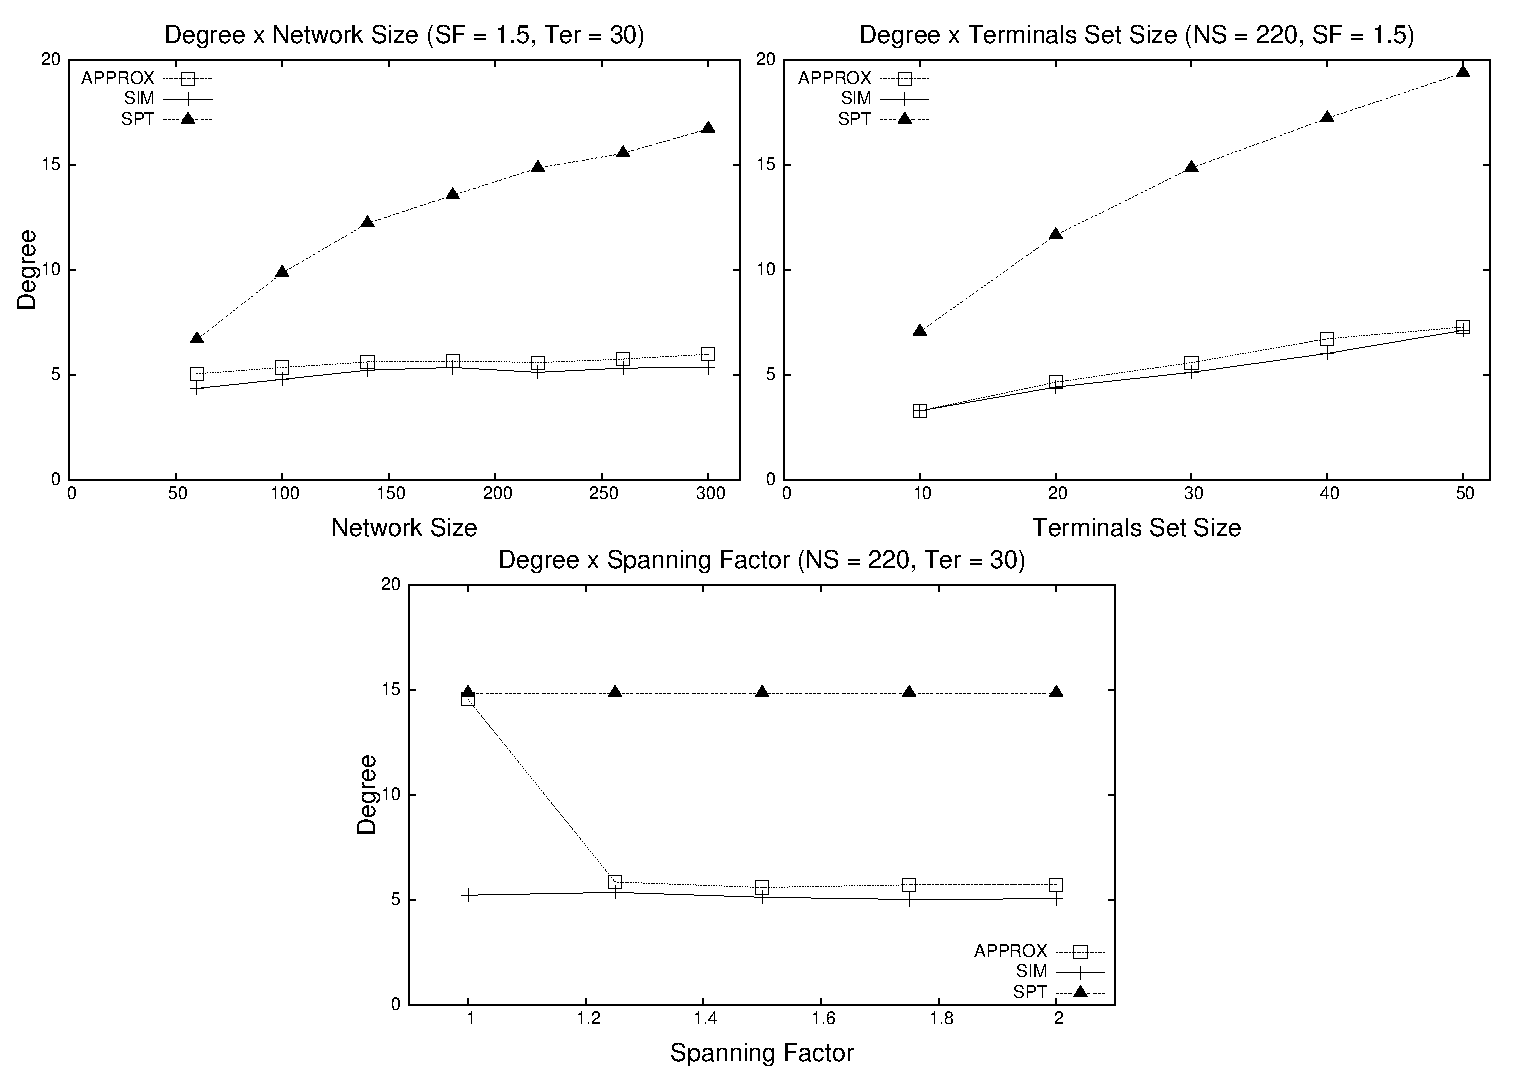
\includegraphics[scale=0.63]{imagens/grau-220-3_graficos_nao_alinhados}
\caption{Maximum out-degree in function of (a) network size, (b) number of terminals, and (c) spanning factor}
\label{fig:degree_abscissae}
\end{figure*}
\begin{figure}[!th]
\centering
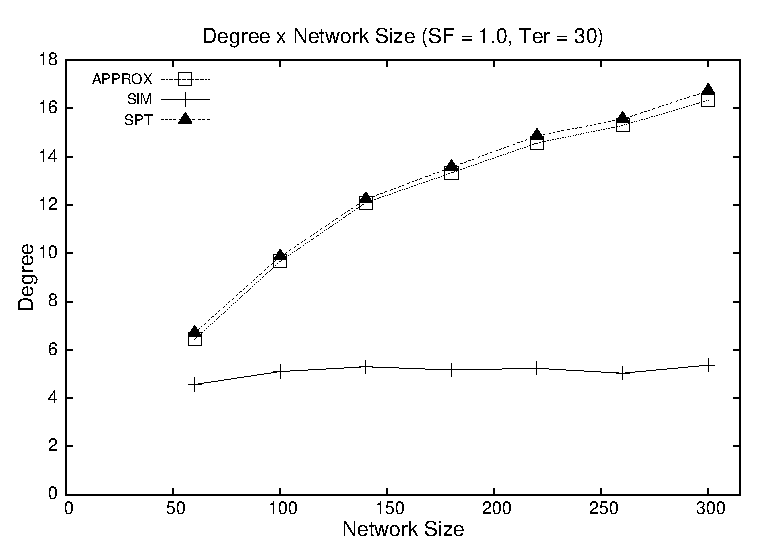
\includegraphics[scale=0.63]{imagens/grau-220-sp1}
\caption{Degree x Network Size when spanning factor is 1}
\label{fig:degree_network-size}
\end{figure}
\begin{figure*}[!th]
\centering
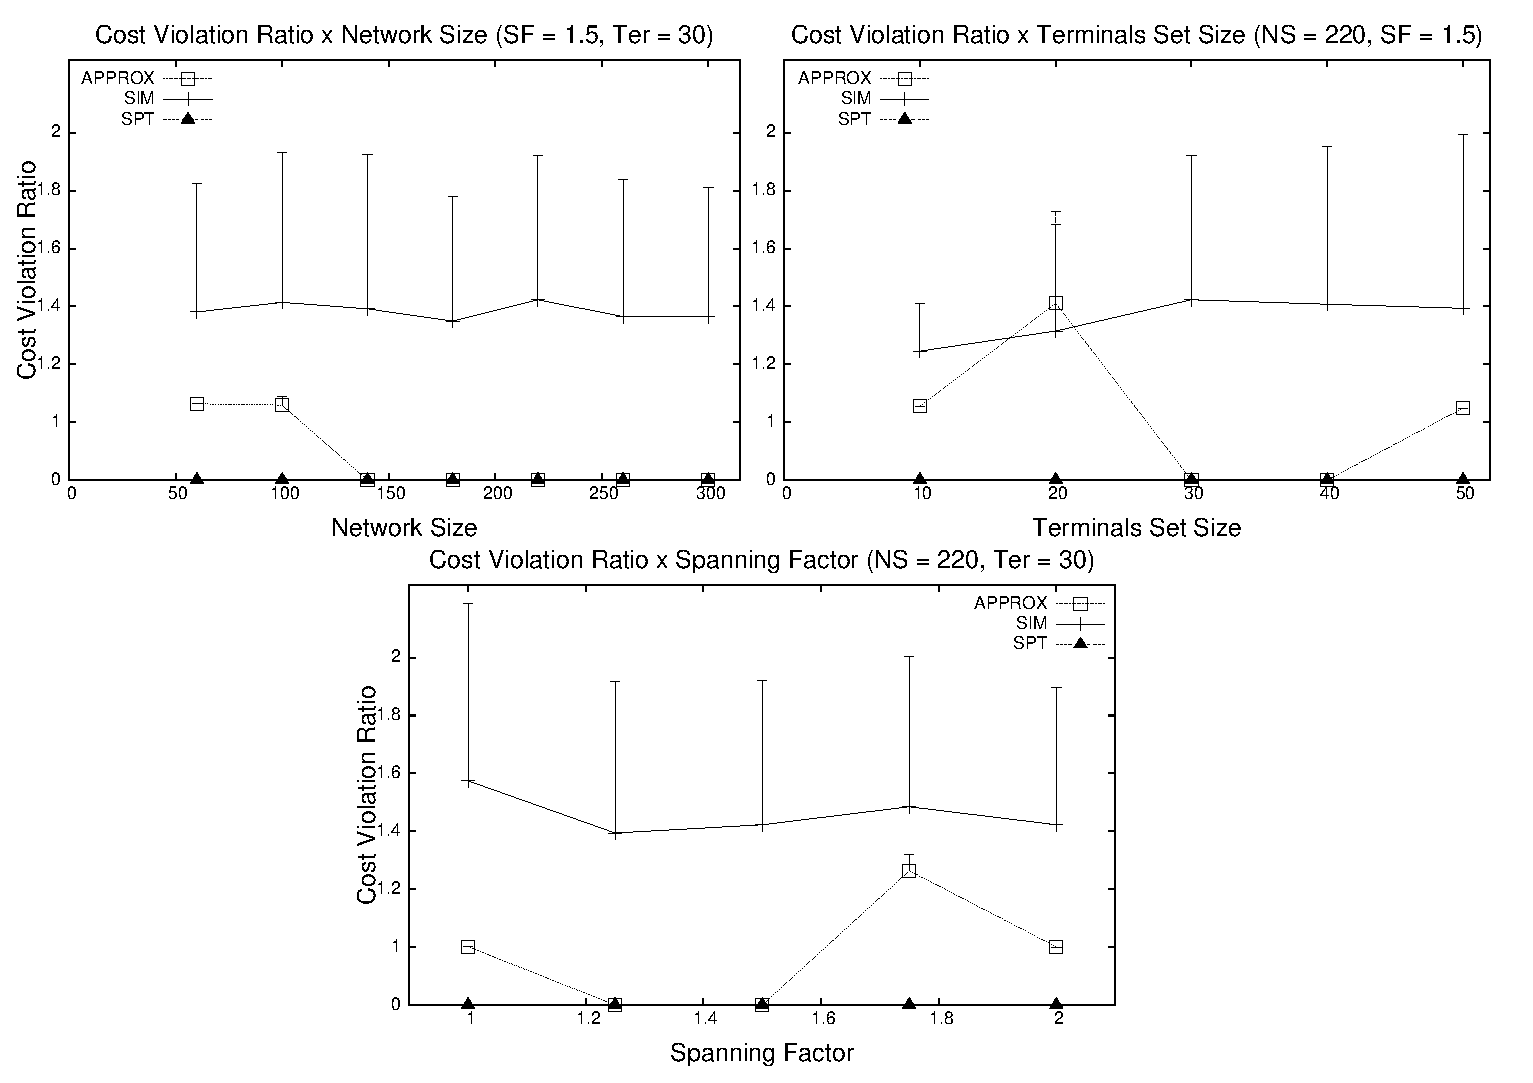
\includegraphics[scale=0.63]{imagens/violatedTerminalsCVR-220-3_graficos_nao_alinhados}
\caption{Cost Violation Ratio in function of (a) network size, (b) number of terminals, and (c) spanning factor}
\label{fig:cvr_abscissae}
\end{figure*}
\begin{figure*}[!th]
\centering
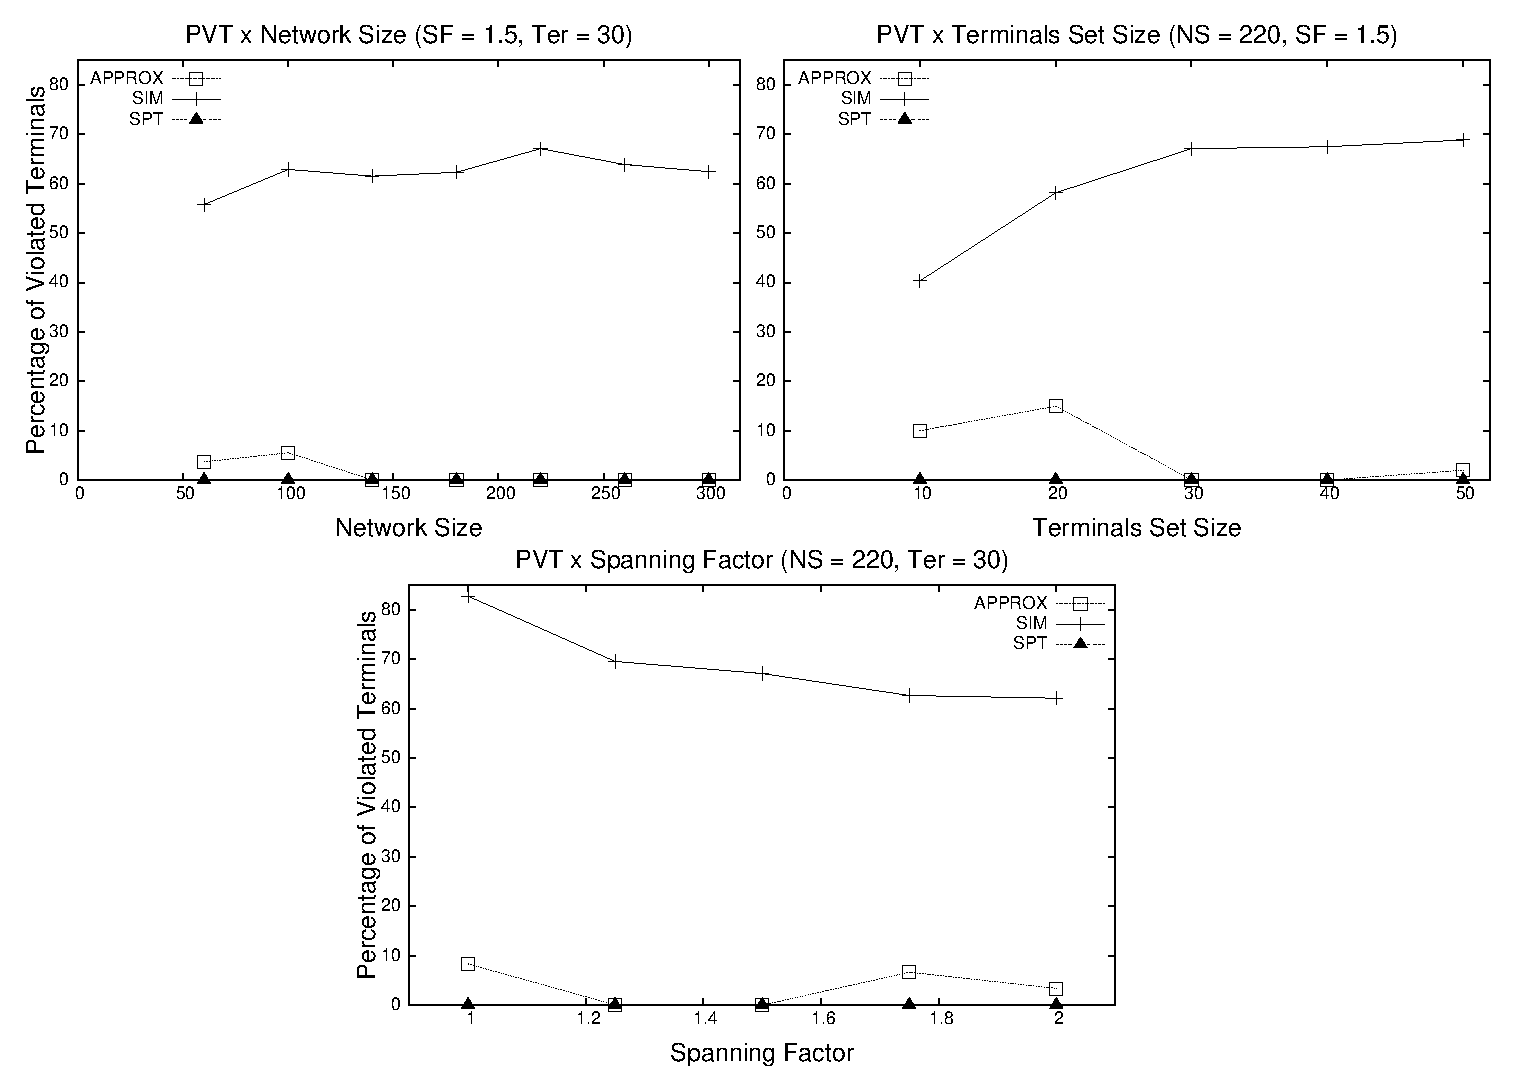
\includegraphics[scale=0.63]{imagens/violatedNodesRatio-220-3_graficos_nao_alinhados}
\caption{Percentage of Violated Terminals in function of (a) network size, (b) number of terminals, and (c) spanning factor}
\label{fig:violated-terminals_abscissae}
\end{figure*}

%Figure \ref{fig:degree_abscissae}c gives us a clue that Algorithm \ref{alg:approximation} suffers a lot when the spanning factor is restrictive. Moreover, 
Since APPROX imitates, in some aspects, the SPT algorithm, we evaluated the algorithms for the specific case of 
spanning factor equal to $1$. 
This graphic is illustrated by Figure \ref{fig:degree_network-size}. Observe that the curve of APPROX  
is very close to the curve of SPT. 
Assuming a spanning factor of 1 corresponds to the situation when the restrictions on the paths from the source node to
the terminals correspond to the minimum cost paths.
As the restrictions are tighter, there will be less paths to choose
%(actually, in the majority of cases it will be only one and the set of paths will correspond to subpaths of a SPT to these terminals) 
leading to the uncovered terminals and respecting the constraints in the second phase of APPROX. This might contribute
to an increase in the degree of nodes. 
%and Algorithm \ref{alg:approximation} tries to do this. This is worsen by the fact that, in the second phase, there will be only very few paths 
%(actually, in the majority it will be only one) leading to the uncovered terminals and respecting the constraints imposed by the modeling of the edges of MSC. 
%So, not only there will be very few available paths to the terminals in the second phase but also the majority of terminals will be in this situation 
%(in part, illustrated by Figure \ref{fig:violated-terminals_abscissae}c), making APPROX behave similarly to SPT. 
On the other hand, SIM is quite good for scalability in this situation too. 
Although both APPROX and SIM apply the algorithm for the MSC problem, only APPROX exhibited behaviour similar to SPT. This might be explained by the restrictions 
on the edges that are allowed to be part of a MSC instance, where for APPROX the restriction considers paths from the source node to the terminal and for SIM the restriction only considers 
the path from a covered node (which is unique) to the terminal. 

%This is corroborated by the low percentage of terminals covered in first phase of the algorithm, showed in Figure \ref{fig:ter_covered} 
%(to be presented later). Due to what was stated before, the number of nodes covered in first phase was low. So, 

Figure \ref{fig:cvr_abscissae} shows the cost violation ratio (CVR) for the three different parameters
(network size, terminals set size and spanning factor). The vertical bars on each point were used to represent MAX\_CVR
(the top of the bars represents its value). On the $y$ axis, the value 0 indicates that at that point no violation for any terminal occurred. 
%the label \emph{N/V} is an acronym for \emph{Not Violated}, which means in that point no violation for any terminal occurred. 
For this metric, it is obvious that SPT will always exhibit the best behaviour (all of its points are on the line $y = 0$), 
as it finds shortest paths. The closer the value to 1, the lesser the violation. 
In Figure \ref{fig:cvr_abscissae}a, the CVR's value for APPROX is quite close to 1 for the first 2 points, 
and no violation occurs for the others. 
The CVR's value for SIM is greater than APPROX, but it is still low (1.4 in average) and it is uniform. In Figures \ref{fig:cvr_abscissae}b and \ref{fig:cvr_abscissae}c, 
the CVR's behaviour is similar to the one presented in Figure \ref{fig:cvr_abscissae}a for both proposed algorithms. Considering APPROX's values, 
in almost half of its abscissa's values no violation occurs and in the other points the CVR's value is close to 1 (except for one point in each graphic). 
Regarding SIM's values, the CVR is again low (between 1.4 and 1.5 in average) and uniform. In the graphics, the behaviour of MAX\_CVR for the algorithms is repeated. 
Regarding the APPROX algorithm, MAX\_CVR is really close to CVR (except for one point in Figure \ref{fig:cvr_abscissae}b) and, in some cases, they are 
almost the same, which it is good because APPROX's worst case is close to the average case. Concerning SIM, the MAX\_CVR is slightly 
higher than CVR, but it is in almost all situations $\le 2$, which is quite acceptable.

CVR measures the quality of violation, but it is important to calculate the amount of violation. PVT 
captures this concept. More specifically, PVT answers the question: when violation occurs, how many terminals violate their constraint? 
The values of PVT are shown in Figure \ref{fig:violated-terminals_abscissae}. 
%Although plotting SPT is unnecessary, we plotted it in order to take its curve as base (mainly for APPROX). 
For all three graphics, the PVT's value is 0 for the same points where no violation 
occurs in Figure \ref{fig:cvr_abscissae}. In Figure \ref{fig:violated-terminals_abscissae}a, the PVT's value for APPROX is quite low (less than 10\%). In fact, 
the behaviour of PVT for APPROX is similar for all the three graphics, where the value exhibited is generally less than 10\%. Concerning SIM, the PVT's value 
is high but it is uniform for the network size (between 60\% and 70\%). 
For SIM, there is a tendency to increase the PVT value with the increse in the terminals set size.
On the other hand, when we vary the spanning factor, the higher the spanning factor, the lower the PVT's value for SIM.

Finally, we evaluated the percentage of scenarios where (at least one) violation occurs (PVR). 
The graphic of PVR is represented by Figure \ref{fig:violated-runs_network-size}. For APPROX, the 
denser the network, the lower PVR is. Additionally, the percentage is no greater than 30\%. Even though this value could be considered, in some senses, to be not  
so low, recall that PVR disregards the percentage of terminals which violate the spanner constraint 
(the run is considered violated even if the constraint is violated for a single terminal) and the amount of violation. The latter is captured by the CVR metric. A variation of the former is captured by PVT metric.
For SIM, PVR has the highest possible value.

\begin{figure}[!th]
\centering
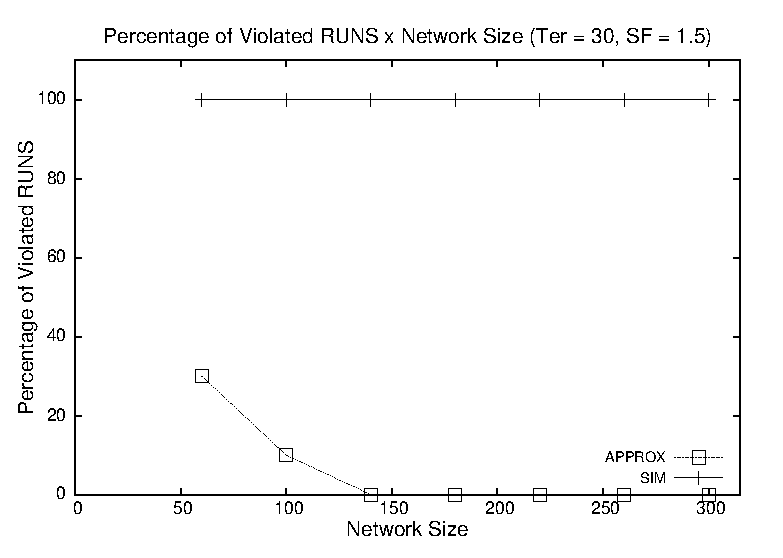
\includegraphics[scale=0.63]{imagens/percViolatedRUNS-ter30sf15}
\caption{Percentage of Violated RUNS x Network Size}
\label{fig:violated-runs_network-size}
\end{figure}

According to our experiments, the maximum out-degree for the proposed algorithms was quite low, except for APPROX in the 
worst scenario when the spanning factor was set to 1 (Figure \ref{fig:degree_abscissae}c). In this scenario, APPROX mimicked SPT's behaviour. 
SIM had uniform behaviour at large, supporting better scalability, and always outperformed APPROX 
in the degree metric. On the other hand, APPROX always outperformed SIM for the CVR, PVT and PVR metrics. More than that, APPROX 
presented very good results for both the quality (CVR) and the quantity (PVT and PVR) of violation. In almost half of abscissa's values (in some situations, more than half) 
no violation occurred. Regarding the quality of violation, when it occurred, the violation was quite low, even in worst cases. The same happened for the 
quantity of violation in the case of APPROX. Considering SIM, although the values were not as so good as for APPROX, 
especially for the quantity metrics, SIM presented very good results for the metric that measures the quality of violation, which is the one that best summarizes 
the analysis of the spanner property. For the CVR metric, the value was quite low (in average 1.4) and even in the worst case it was low (in most cases limited by 2). Furthermore, the values achieved by CVR exhibited an uniform behaviour in general.

%In the next chapter, we are going to conclude the thesis and present future work.
In the next chapter, we discuss extensively the related work, presenting the main results. Moreover, we argue why DSMDStP is 
a new problem, giving the differences between our problem and the related ones.

%In the next chapter, we are going to describe how we could improve the degree guarantee for APPROX through a new modeling of MCG. This new modeling 
%is based on the concepts of \emph{submodular function} and \emph{matroid}. This improvement would be possible due to the results presented in \cite{Calinescu2011}, 
%but doing this we would turn our algorithm into a randomized one.

\xchapter{Related Work}{}
\label{sec:related}
\acresetall

  %o trabalho de Chen2004 afirma que o problema de multicast eh o mesmo que o problema de Steiner tree
In this chapter we present an extended up-to-date range of related work, from network design problems that address single properties to, similar to our case, 
problems that address multiple properties. We start by motivating for Steiner trees and spanners. Then, we discuss the related work addressing the properties of interest (spanner and degree) in 
Euclidean Space (Section \ref{sec:euclidean_space}) as well as in (undirected and directed) graphs (Section \ref{sec:properties_in_graphs}). Finally, we explain why DSMDStP 
is a new problem, giving its differences from related work (Section \ref{sec:DSMDStP_new_problem}).

Steiner trees are typically related to optimizing multicasting (for example, \linebreak 
\cite{Sun1995,Raghavan1998,Feng1999,Parsa1998,Zhengying2001,Wang2009,Wang2005,Chen2004}). 
In classical Steiner tree problems, the goal is to minimize the cost of the tree while satisfying certain constraints.

Spanners are applied in many scenarios. For instance, spanners can be used to support efficient routing. Spanners 
allow routing protocols to store smaller routing tables while packets' headers are still small, 
%since spanners allow a tradeoff between packets' headers and routing table (the lesser the headers' size - fewer routing information is stored in the packet - the greater the rougting table -
since spanners allow a tradeoff between packets' headers and routing table 
%(when shortest paths are used to route, the headers' size can be the least - only the destination label is stored in the packet - so the routing table can be the greatest - each node need to know how to route a packet for every possible destination - and vice versa) 
(when packets are routed through shortest paths, each node has to store a complete routing table or the packet's header has to contain a complete description of the 
shortest path; spanners allow the tradeoff mentioned before as they use paths with small stretch factors rather than routing through shortest paths) 
\cite{Thorup2001}. (Geometric) spanners are also 
applied in wireless networks to decrease energy expenditure \cite{Schindelhauer2007} (for other applications of geometric spanners, see \cite{Narasimhan2007}). 
Spanners are also commonly used to approximate 
shortest path distances \cite{Feigenbaum2008}. Since calculating shortest paths is common for classical shortest path algorithms, 
approximating distances is of great utility \cite{Feigenbaum2008}. 
Motivation for the adoption of spanners in shortest path algorithms can also be seen in \cite{Elkin2001}.
%Moreover, spanners are applied in shortest path algorithms due to two reasons \cite{Elkin2001}: 
%their convenience in implementing distributed algorithms, since the spanner structure is part of the network itself so the algorithm can execute on the spanner itself; 
%and the second reason \cite{Elkin2001} occurs when the use of an edge by a path incurs a cost. So, it is desired to limit the number of edges used by the path. The 
%number of edges used in building the paths is limited by the size of the spanner. 

In a similar way to this last application of spanners, they are also 
applied in distance oracles \cite{Baswana2006,Thorup2005}. In \cite{Baswana2006}, the authors state that in many applications the objective is 
not to compute all distances (the same as shortest paths) but to be able to retrieve distance values in an efficient way. This can be done through some kind 
of preprocessing of the input graph. Due to the complexity of the traditional shortest path algorithms, researchers have been trying to find out structures 
which report approximate distance values instead of the exact values. This motivates the works on \emph{t-approximate distance oracles}, where for 
a pair of vertices $(u,v)$ in the input graph $G$, the value returned by the oracle is $\ge dist(u,v,G)$ and $\le t \cdot dist(u,v,G)$.

Spanner tree, a restricted kind of spanner, is of great importance too. According to \cite{Liebchen2008}, spanner trees are used in telecommunications since 
they allow routing protocols to be simpler. They are also used as a model for broadcast \cite{Peleg2000} and, in similar way to Steiner trees, 
spanners trees can be used in message multicasting. In the literature, there are also references to their application in solving 
some kinds of linear systems of equations problems \cite{Elkin2005} and in finding approximation solutions to the bandwidth minimization problem \cite{Venkatesan1997}.

%Spanners are applied in a lot of scenarios, e.g., efficient routing \cite{Thorup2001}, approximating shortest path distances \cite{Feigenbaum2008,Elkin2001}, 
%as well as for distance oracles \cite{Baswana2006,Thorup2005}. (Geometric) spanners are also applied in wireless networks (for other applications of geometric 
%spanners, see \cite{Narasimhan2007}). Tree spanners have also a variety of applications, e.g., telecomunications scenarios since they turn routing protocols more simple \cite{Liebchen2008}, 
%solving symmetric diagonally dominant linear systems of equations \cite{Elkin2005}, as a model for broadcast \cite{Peleg2000}, and they are used 
%to find approximate solutions to the bandwidth minimization problem \cite{Venkatesan1997}.


The Steiner tree problems addressed in \cite{Raghavan1998,Feng1999,Sun1995,Parsa1998} involve a single constraint, a cost bound  
on the paths between a source node and the terminals (to model maximum transmission delay).
% ?? tirei a referencia Wang2009 no ultimo \cite no paragrafo anterior
%In \cite{Wang2005,Chen2004} the authors take into consideration both delay and degree constraints.
%??Wang2005 - so tive acesso a primeira pagina do artigo
In \cite{Chen2004} the authors take into consideration both delay and degree constraints.  
In \cite{Chen2004}, the authors assume undirected graph and do not guarantee that the delay constraints will be respected. Additionally, 
the problem involves a single delay constraint, which applies to a subset of nodes. 
Degree constraints arise in scenarios in communication networks to address resource limitations in 
routers and switches and to balance load during multicast operations. 
%In \cite{Wang2005,Chen2004}, the same maximum delay is associated with each terminal. The authors present heuristics based on genetic algorithms.   
%In particular, the algorithm in \cite{Chen2004} does not guarantee that the delay constraints will be satisfied.
%The association of different delay constraints with different terminals (and minimization of the tree cost) is addressed
%in \cite{Parsa1998,Zhengying2001}. This is typically motivated by the existence of different types of terminals or 
%quality-of-service requirements of distinct applications.

\section{Works that consider Spanner and Degree in Euclidean Space}
\label{sec:euclidean_space}
Much previous work has addressed network design problems with more than one property (including being a tree, the spanner property, bounded maximum degree, and others) 
as we do \cite{Arya1995,Dinitz2008,Kortsarz1999}. All these mentioned works assume an Euclidean space, which restricts the applicability of their work 
to scenarios where geometric relations hold as well as associating a different cost based on the direction of the edge is not allowed, as directed graphs are not allowed to be modelled. 
Other works address degree too \cite{Chan2003,Fekete1997,Monma1991,Lukovszki1999,Farshi2007,Lukovszki2006,Grunewald2002}. But they also assume an Euclidean Space.

%Much previous work has addressed network design problems with more than one property (including being a tree) as we do. In \cite{Arya1995}, the authors address the problem of generating 
%a network with bounded maximum degree, constant stretch factor and low weight. Networks with these properties are called \emph{narrow}, \emph{shallow} and 
%\emph{light} respectively in network design literature. The resulted graph in \cite{Arya1995} is not a tree. Shallow-light trees are addressed in \cite{Dinitz2008,Kortsarz1999}. 
%Besides the spanner property, these trees are also guaranteed to have a weight not much heavier than the minimum spanning tree (the \emph{light} property). 
%In \cite{Dinitz2008}, besides being shallow and light, the generated trees are low (the tree's height is bounded). The authors also show that it is possible to generate two kinds of 
%trees with a compromise relation between the weight and the height. In \cite{Kortsarz1999}, the authors give an approximation solution for a Steiner tree problem 
%with a parameterized  
%height and minimum weight. 

%Other works address degree too. In \cite{Chan2003,Fekete1997,Monma1991}, the authors deal with the problem of generating narrow-light trees. 
%In \cite{Chan2003}, the authors give an approximation solution for the 
%minimum spanning tree problem with parameterized  
%degree. In \cite{Fekete1997}, the authors give an approximation algorithm for a problem similar to the last mentioned problem (the one addressed in \cite{Chan2003}), 
%but they allow the degree parameter to be different for each node. The authors of \cite{Monma1991} study some spanning tree problems, including the minimum 
%spanning tree with bounded maximum degree. Other kind of trees studied in the literature are the so called \emph{single-sink spanners} \cite{Lukovszki1999,Farshi2007,Lukovszki2006,Grunewald2002}. 
%These trees are characterized by respecting the parameterized root-stretch factor and having low height and bounded maximum degree. In \cite{Lukovszki1999}, 
%the authors work with fault-tolerant single-sink spanners. The authors of \cite{Farshi2007} performed experimental studies of spanners, including single-sink spanners. 
%In \cite{Lukovszki2006,Grunewald2002}, the authors are concerned with keeping effective use of resources in networks through topology control. 

\section{Works that consider Spanner and Degree in (Directed and Undirected) Graphs}
\label{sec:properties_in_graphs}
More spanner and degree problems on graphs are addressed in \cite{Fomin2011,Dinitz2011,Berman2011,Elkin2011b,Hajiaghayi2009,Naor1997} and 
\cite{Khandekar2011,Goemans2006,Singh2007,Elkin2006,Bansal2009,Nutov2011,Feder2006,Ravi1992} respectively. These work assume undirected graphs, which is a restricted case of our 
more general assumption of directed graphs. 

On the other hand, the authors in \cite{Dinitz2011,Naor1997,Berman2011} deal with related problems in directed graphs. Their 
works differ from ours as the resulted graph is not a tree or the authors aim at minimizing a different function (e.g., the number of edges, the total cost of the tree). The works 
in \cite{Bansal2009,Nutov2011} address tree problems with degree restrictions in directed graphs too. They are interested in guarateeing k-connectivity. 
In these works, the authors aim to satisfy the degree restriction imposed to each node rather than minimize the maximum degree. 
Additionally, they do not consider the spanner property. The problems addressed in \cite{Feder2006} are simitar to the ones addressed in the former papers. The authors 
consider the problem of minimizing the maximum degree but they do not consider the spanner property neither.

%More spanner (or related shallow) and degree problems on graphs are addressed in \cite{Fomin2011,Dinitz2011,Berman2011,Elkin2011b,Hajiaghayi2009,Naor1997} and \cite{Khandekar2011,Goemans2006,Singh2007,Elkin2006,Bansal2009,Nutov2011,Feder2006} respectively. 
%In \cite{Fomin2011}, the authors address the problem of generating \emph{k}-spanners (spanners with the stretch factor of $k$) that are also trees. In \cite{Fomin2011}, 
%the authors are concerned with generating trees where the stretch factor is guaranteed between any pair of nodes rather than between only the source node and the other nodes.
%This problem is NP-Complete even if the input graph is planar. The authors show that if the input graph has a known bounded maximum degree, it is possible to decide 
%in polynomial time if the graph has a k-spanner tree with bounded treewidth. 
%They assume undirected graphs. In \cite{Elkin2011b}, the authors are interested in the problem of generating spanner and light trees in undirected graphs. 
%In \cite{Hajiaghayi2009}, the authors deal with generating Steiner trees with bounded path costs 
%that are light. 

%On the other hand, the authors in \cite{Dinitz2011,Naor1997,Berman2011} deal with related problems in directed graphs. In \cite{Naor1997}, the authors attack the 
%problem of generating light spanning trees with bounded path costs. The authors in \cite{Dinitz2011,Berman2011} 
%attack the problem of generating spanners with the minimum number of edges, where the input graph is directed and its edges have arbitrary cost. 
%Their solutions are not trees. The authors of \cite{Berman2011} give an approximation algorithm for the directed Steiner forest problem, where the 
%objective is to minimize the cost of the forest. In \cite{Khandekar2011}, solutions are analyzed and proposed for several network design problems 
%with degree constraints. One of these problems is the \emph{Minimum Degree p-Arborescence} problem, where the objective is to find an arborescence that 
%covers $p$ terminals (where $p \le |T|$) and has minimum out-degree (the same as bounded maximum out-degree). In \cite{Elkin2006}, one of the results is a solution for the directed 
%minimum-degree Steiner tree problem (with $p = |T|$), consisting of a specific case of the problem addressed in \cite{Khandekar2011}. 

%In \cite{Goemans2006} an algorithm is proposed for the minimum spanning tree with 
%maximum degree $d^*+2$, where $d^*$ is the optimum degree. This result is improved in \cite{Singh2007} to $d^*+1$. Both works assume undirected graphs. 
%The authors of \cite{Ravi1992} propose solutions for the minimum-degree Steiner tree problem for undirected graphs. Regarding degree 
%constraints, the authors of \cite{Bansal2009,Nutov2011} propose approximation solutions for problems in network design with degree restrictions, among them  
%the degree-bounded (the same as bounded maximum degree) arborescence problem. In \cite{Feder2006}, the authors propose solutions for similar problems to those tackled in \cite{Bansal2009,Nutov2011} 
%concerning survivable network, but they are the first to consider k-node connectivity instead of only k-edge connectivity.

\section{Our Problem: The novelty in DSMDStP}
\label{sec:DSMDStP_new_problem}

Our work differs from related work as in our case we consider directed graphs instead of working in metric spaces or assuming undirected graphs. Additionally, we aim to find Steiner trees, 
a more general case of spanning trees. Moreover, besides building a Steiner tree with bounded maximum degree in directed graphs, we also address the $k$-spanner 
property, more specifically, 
%a tree whose paths from source node to terminals have stretch factor of $k$ related to the paths between these nodes in original directed graph. 
single-sink k-spanner trees, where $k$ is a parameter of the problem (instead of a bound achieved by a solution to the problem). 

The closest works to ours are \cite{Elkin2009,Elkin2011,Elkin2006,Khandekar2011}. In \cite{Elkin2009,Elkin2011}, the authors address the problem of building narrow-shallow-low-light trees. 
The authors thus address the problem of generating trees with parameterized root-stretch factor 
%\footnote{Some works that generate spanner trees guarantee the spanner property between any pair of nodes from the tree rather than guaranteeing the property only from the source node to the other nodes, as in \cite{Elkin2009,Elkin2011}} 
and bounded maximum degree, as we do, but they consider two additional properties (generation of 
\emph{low} and \emph{light} trees).
However, their work builds a spanning tree rather than a Steiner tree and they consider metric spaces. Our assumptions are more
general, as we do not restrict our problem to metric spaces. Additionally, 
the authors' work provides a constant root-stretch factor, similarly to other works where shallow trees are generated, rather than supporting a parameterized stretch factor. 
The authors in \cite{Elkin2006,Khandekar2011} address the problem of minimizing the out-degree of directed graphs in Steiner tree problems. 
In \cite{Elkin2006}, similar to our work, the problem consists in covering all the set $T$ of terminals, 
while in \cite{Khandekar2011} the problem is generalized as the objective is to cover $p$ terminals, where $p \leq |T|$. In both works, the authors do not consider the spanner property. They also address problems 
somewhat similar to ours, where besides minimizing the maximum degree it is required to limit the height of the tree. So, they are interested in limiting the 
number of hops, which differs from our spanner property. To the best of our knowledge, our work is the first attempt to address the problem of building a Steiner 
tree in directed graphs with limited maximum degree and with a parameterized root-stretch factor.

%Our work differs from related work since in our case 
%the optimization function is the maximum out-degree instead of the total cost of the tree and
%different terminals might have different cost constraints. Finding a multicast tree taking into consideration
%these two aspects together corresponds, to the best of our knowledge, to a new problem, which we call DCCMDSt.

%Our approximation algorithm might violate terminal constraints. The authors in 
%\cite {Oliveira2005} state that when solutions to classical Steiner tree problems are extended to consider delay constraints, the approximations are 
%no longer guaranteed. The authors argue that adding the delay contraints makes the problem much harder to 
%approximate. Delay constraints are, for example, violated in the algorithms in \cite{Chung1997,Kompella1993} and no bound to delay violation
%is provided. In our work, the terminal constraints are violated by a known additive factor. 

%Another important point is that in algorithms in which delay constraints are satisfied (for example, \cite{Feng1999,Sun1995}), 
%the delay is guaranteed at the expense of adding new edges to form a new path that respects the delay 
%beyond those in shortest cost paths. So minimizing degree and satisfying terminal constraints
%seems to be conflicting goals. Our work is the first attempt to address degree minimization and different terminal constraints in the Steiner tree problem.
%Our algorithm provides guarantees on maximum node degree.

\subsection{Limitation in the Results}
Our algorithms are not able to guarantee the root-stretch factor $k$ for all paths from the source node to the terminals. 
%, which differ from the majority of works that address spanner property in trees \cite{Dinitz2008,Kortsarz1999,Elkin2009}, where the root stretch factor is a constant of $(1+\epsilon)$, for any fixed $0 < \epsilon < 1$. 
Our approximation algorithm and heuristic give a root-stretch factor of 
$k \cdot \left(1 + \frac{max_{t\in T}\{dist(s,t,G)\}}{min_{t \in T}\{dist(s,t,G)\}}\right)$ and $k \cdot (\lfloor\sqrt{|T|}\rfloor+2)$ respectively.
%, where $dist_{max} = max\{dist(s,t,G) | t \in T\}$ and $dist_{min} = min\{dist(s,t,G) | t \in T\}$. 
However, as argued in the introduction, 
in the experiments the cost of the generated paths is much lower than the provided upper bounds.
%due to the way the algorithm works, we were able to give an empiric compromise relation between the average maximum degree and the 
%final costs of the paths in the Steiner tree.

\subsection{The Base Algorithmic Tool for the Proposed Solutions: The MSC Problem}
Our algorithms are based on the algorithm presented in \cite{Elkin2006}. In \cite{Elkin2006}, the goal is to compute a schedule
with a minimal number of rounds that delivers a message from a given node to all the terminals. The problem is called \emph{Directed Telephone Multicast Problem}. 
Our approximation algorithm follows the same steps as in 
\cite{Elkin2006}, but we use different criteria for defining some of the used concepts, such as $\sqrt{k}$-bad nodes, and for the
construction of the instance of the Multiple Set-Cover (MSC) problem. The bound on the degree
is obtained in exactly the same way as in \cite{Elkin2006}. The heuristic SIM deviates from the algorithm in \cite{Elkin2006}, as it is based on an iterative application
of the MSC problem (instead of applying this problem only once, as in our algorithm and in \cite{Elkin2006}).

The Multiple Set-Cover (MSC) problem was stated for the first time in \cite{Elkin2003}. A solution for this problem
was presented in \cite{Chekuri2004}. 
%(actually, the journal version \cite{Elkin2006} (the one used by us) uses the solution presented in \cite{Chekuri2004}, and the conference paper \cite{Elkin2003} 
%uses a different solution). 
In \cite{Chekuri2004}, MSC is called \emph{Set Cover with Group Budgets} (SCG). 
The MSC problem can be generalized by the problem called \emph{Maximization of Monotone 
Submodular Function subject to Matroids Constraint}, which was addressed in \cite{Calinescu2011}. 
%We can generate a variation of our algorithm with an improvement on the maximum out-degree (with high probability) by using this more general problem and the algorithm provided in \cite{Calinescu2011}.
However, our goal in this dissertation is to present a deterministic algorithm. 
We will discuss this in greater detail in Appendix \ref{sec:matroid}. 

%In the next chapter we define DSMDStP as well as to prove that it is not approximable sublogarithmically.
In the next chapter, we conclude the dissertation and present future work.

\xchapter{Conclusion}{}
\label{sec:conclusion}
\acresetall

%ALTEREI PARAGRAFO
In this dissertation we presented a version of a Steiner tree problem called \emph{Directed k-Spanner with Minimum Degree Steiner Tree Problem} (DSMDStP). 
Unlike commonly defined Steiner tree problems, in DSMDStP we are interested in minimizing 
the maximum out-degree of the arborescence while respecting the terminals spanner constraints. We assume as input a directed graph.
To the best of our knowledge, these properties characterize \mbox{DSMDStP} as a new problem.
We showed that \mbox{DSMDStP} is not approximable sublogarithmically (unless $NP \subset DTIME(n^{\log \log{n}})$) and described an approximation algorithm and a heuristic to it. 
For both proposed algorithms, we analyzed their complexity.

The approximation algorithm is based on the algorithm described in \cite{Elkin2006}. The algorithm generates an arborescence $\mathcal{A}_f$ 
with maximum degree $2\sqrt{|T|} + 2 + O(\log{|T|})\cdot d^*$, where $d^*$ is the maximum degree of an optimum arborescence.
This seems a reasonable limit, as 
%it was proved in \cite{Fraigniaud2001} that MDST, a restricted version of 
DSMDStP does not admit a sublogarithmic approximation.
Additionally, in $\mathcal{A}_f$ the paths from $s$ to each terminal $t$ have cost $\le k \cdot ( dist(s,t,G) + dist(s,t_{max},G))$, where $t_{max} \in \{t' | t' \in T \land (\forall t'' \in T: dist(s,t'',G) \le dist(s,t',G))\}$. 
Although the algorithm can violate the spanner constraint, 
this only happens to terminals covered in the second phase of the algorithm. 
%In Section \ref{sec:related} we argue that adding the terminal constraints to the problem makes it much harder to approximate.

%ALTEREI PARAGRAFO
The heuristic, called SIM, is based on an iterative application of an algorithm for the MSC problem. SIM does not provide guarantee on maximum node degree. 
However, in our experiments SIM provided lower maximum node out-degree than the approximation algorithm. 
In the final arborescence, the path from $s$ to $t \in T$ has cost $ \le (|T| + 2) \cdot k \cdot dist(s,t,G)$. 
%Different from the approximation algorithm, beyond $k$, the paths' final cost depend only on shortest distance
%, i.e., beyond $k$ it only depends on the cost constraint of $t$. In our simulations, SIM generates trees with maximum degree much lower than the maximum degree in shortest path trees.

The experiments presented quite good results for both proposed algorithms. Regarding the node out-degrees, both the approximation algorithm and SIM yielded low
maximum out-degree and they outperformed the results of a shortest path tree algorithm (SPT). Additionally, SIM has always outperformed the approximation algorithm 
and it has a uniform behaviour, what contributes to scalability. 
On the other hand, the approximation algorithm always outperformed SIM in metrics concerning the spanner constraint. Moreover, in half of the situations 
no violation occurred. The metrics addressing the spanner constraint measured the quality and the quantity of violation. Even when violation occurred, 
these metrics showed that the approximation algorithm violated by low factors. 
Although SIM did not present as good results as the approximation algorithm, 
concerning the metric that addresses the quality of violation (how much the violation occurred), the results were also 
quite good, since on average the violation was by a factor of 1.4 and in worst case by a factor of 2, which are quite acceptable.

%Concerning the spanner property, in average, the approximation algorithm satisfied 
%the spanner constraint, which led us to conclude the theoretical bounds are pessimistic. Even SIM not respecting the spanner constraint, it violated the constraint, 
%in average, by low factors and again exhibited uniform behaviour. So, SIM performed very good for both metrics.

We also described how we can improve (with high probability) the degree guarantee for the approximation algorithm. This can be done through the concepts of \emph{submodular functions} 
and \emph{matroid}. More specifically, we can solve DSMDStP using an instance of a problem called MCG. 
The improved result can be achieved by modelling MCG as a problem of \emph{maximizing a monotone submodular function subject to partition matroid constraint} and using the algorithm presented in \cite{Calinescu2011} to solve it. 

\section{Future Work}
%Although we aimed at proposing a solution for DSMDStP where the spanner constraints were satisfied, we could not do it in this work. 
%So, a possible future work could be to investigate new algorithms to try to improve the resutls. %Our results ...

A possible future work could be to investigate new algorithms to try to improve the resutls, mainly concerning the spanner property. It is important to mention that 
we do not know if DSMDStP admits a solution.

Turning the solutions into distributed ones would be challenging and another possible future work. 
%A distributed solution would allow us to apply it 
%in scenarios where distributed algorithm is a requirement or really important, such as in Wireless Sensor Networks. Besides this, a distributed solution 
Distributed algorithms are necessary in some scenarios, such as in Wireless Sensor Networks. Besides this, a distributed solution 
is more scalable than a centralized one, which is an important property.

We argued in Appendix \ref{sec:matroid} how we could improve the degree guarantee of the proposed approximation algorithm by modelling the problem 
(actually, the subproblem MCG) through the concepts of submodular functions and matroids. But doing this, our algorithm would be a probabilistic one. Although being probabilistic, 
it would be interesting to see by how much the degree is improved in practice. So, another possible future work would be to solve the MCG problem 
through the solution proposed in \cite{Calinescu2011} and compare the results with the ones presented in this dissertation.
%implementar matroid

%\begin{itemize}
  %\item Try to improve the solution in order to respect the spanner constraint.
%\end{itemize}

%\include{desenvolvimento}
% Eh aconselhavel criar cada capitulo em um arquivo separado, digamos
% "capitulo1.tex", "capitulo2.tex", ... "capituloN.tex" e depois
% inclui-los com:
% \include{capitulo1}
% \include{capitulo2}
% ...
% \include{capituloN}
%
% Importante: 
% Use \xchapter{}{} ao inves de \chapter{}; se não quiser colocar texto antes do inicio do capitulo, use \xchapter{texto}{}.

%\xchapter{Introdu\c{c}\~{a}o}{Este eh o primeiro cap\'{\i}tulo, onde eu conto toda a historia deste trabalho, o problema, a solu\c{c}\~{a}o, etc.}

% É recomendável utilizar `\acresetall' no início de cada capítulo para reiníciar o contator de referências às siglas.
%\acresetall 

%\section{Se\c{c}\~{a}o}
%Trabalho do  \ac{PPGM}. Bolsa do \ac{CNPq}.
%
%\begin{figure}[h]
%    Figure
%    \caption[As siglas também funcionam nas legendas]{As siglas também funcionam nas legendas, seja na forma de sigla \ac{CNPq}, seja na forma completa \acf{PGCOMP}.}
%\end{figure}
%
%\lipsum
%
%\subsection{Uma Subse\c{c}\~{a}o}
%\acresetall
%Texto para mostrar como o \verb|\acresetall| funciona \ac{CNPq}, \ac{PGCOMP}. Ele reseta os contadores e faz a sigla aparecer na forma estendida novamente.
%
%\subsection{Outra Subse\c{c}\~{a}o}
%
%Texto  \acf{CNPq}, \acf{PGCOMP}.
%
%
%\xchapter{Revis\~{a}o Bibliogr\'{a}fica}{Neste cap\'{\i}tulo eu apresento todo o material que eu estudei durante a elabora\c{c}\~{a}o do trabalho.}
%
%\lipsum
%
%Livro \cite{demeyer2008} e  livro \cite{raymond1999}.
%
%\xchapter{Exemplos}{} %sem preambulo
%
%A numera\c{c}\~{a}o de figuras \'{e} sequencial, dentro do cap\'{\i}tulo. Ver Figura \ref{default-regular1} e Figura \ref{default-regular2}.
%
%A numera\c{c}\~{a}o de tabelas \'{e} sequencial, dentro do cap\'{\i}tulo. Ver Tabela \ref{default-table1} e Tabela \ref{default-table2}.


%\section{Exemplos de Figura}
%
%\begin{figure}[htbp]
%\begin{center}
%  
\includegraphics[scale=0.5]{ufba.eps}
%\caption{Bras\~{a}o da UFBA - Menor.}
%\label{default-regular1}
%\end{center}
%\end{figure}
%
%\begin{figure}[htbp]
%\begin{center}
%  
\includegraphics[scale=0.75]{ufba.eps}
%\caption{Bras\~{a}o da UFBA - Maior.}
%\label{default-regular2}
%\end{center}
%\end{figure}
%
%\lipsum
%
%\section{Exemplos de Tabela}
%\subsection{Uma Tabela}
%\begin{table}[htbp]
%\caption{Uma tabela com 3 linhas e 2 colunas.}
%\begin{center}
%\begin{tabular}{|c|c|} 
%\hline
%elemento 11 & elemento 12 \\ \hline
%elemento 21 & elemento 22 \\ \hline
%elemento 31 & elemento 32 \\
%\hline
%\end{tabular}
%\end{center}
%\label{default-table1}
%\end{table}%
%
%\lipsum
%
%\begin{table}[htbp]
%\caption{Uma tabela com 3 linhas e 3 colunas.}
%\begin{center}
%\begin{tabular}{|l|c|c|} 
%\hline
%elemento 11 & elemento 12 & elemento 13\\ \hline
%elemento 21 & elemento 22 & elemento 23\\ \hline
%elemento 31 & elemento 32 & elemento 33\\
%\hline
%\end{tabular}
%\end{center}
%\label{default-table2}
%\end{table}%
%
%\xchapter{Outro cap\'{\i}tulo}{} %sem preambulo
%\lipsum


%% Parte pos-textual
\backmatter

% Bibliografia
% É aconselhável utilizar o BibTeX a partir de um arquivo, digamos "biblio.bib".
% Para ajuda na criação do arquivo .bib e utilização do BibTeX, recorra ao
% BibTeXpress em www.cin.ufpe.br/~paguso/bibtexpress
\bibliographystyle{abntex2-alf}
\bibliography{dissertation}

% Apendices
% Comente se naoo houver apendices
\appendix

%\chapter{An alternative to improve the degree guarantee for the approximation algorithm}
%\chapter{An alternative to solve DSMDStP}
\xchapter{Discussion about how to approach DSMDStP through an alternative way}{}
\label{sec:matroid}

In this appendix we comment on how we could approach the MCG problem through an alternative way and the impact of this new approaching for the DSMDStP. 
This new modeling of MCG would allow us to decrease the maximum degree for the DSMDStP. 
%In this appendix we comment on the impact of solving DSMDStP through an alternative way. 
%In this appendix we discuss how we could improve our degree guarantees for the proposed approximation algorithm. 
In order to do this, we would model 
the MCG problem through the concepts of \emph{submodular functions} and \emph{matroid}. We briefly present these concepts and show how MCG could 
be modeled through them. Although there is a result that allows the improvement of the degree guarantee of our problem, this would turn our algorithm in 
a probabilistic one, as the presented result for this new modeling of MCG is a randomized algorithm. 
The results discussed here are a mere conjecture.

%ALTEREI PARAGRAFO
As mentioned in \cite{Calinescu2011}, the MCG problem \cite{Chekuri2004} could be addressed through the concepts of \emph{monotone submodular functions} and 
\emph{matroids}. More specifically, MCG can be modeled as a problem of maximizing a monotone submodular function under matroid constraint. 
As we can solve MSC using MCG, improvements on solution to MCG extend to MSC as well \cite{Elkin2006} (the SCG problem in \cite{Chekuri2004}). Let $X$ be a ground set of $n$ elements. A function $f: 2^{X} \rightarrow \mathbb{R}^+$ is \emph{submodular} iff: 

\begin{center}
$f(A \cup B) + f(A \cap B) \le f(A) + f(B)$,
\end{center}

for all $A,B \subseteq X$ \cite{Schrijver2003}. $2^X$ represents the set of all subsets of $X$, including the empty set and $X$ itself. 
$f$ is called \emph{monotone} if $f(A) \le f(B)$, for all $A \subseteq B$. In order to address the \emph{matroid} 
concept, besides a ground set $X$ we need the concept of an \emph{independence family} $I \subseteq 2^{X}$, a family of subsets that is downward closed, which 
means that $A \in I$ and $B \subseteq A$ implies that $B \in I$. A \emph{matroid} is a pair $M = (X,I)$ where $I \subseteq 2^{X}$ and

\begin{align*}
&\tag{i} \forall B \in I, A \subset B \Rightarrow A \in I.\\ 
&\tag{ii} \forall A,B \in I; |A| < |B| \Rightarrow \exists x \in B \setminus A; A \cup x \in I.
\end{align*}

The problem addressed in \cite{Calinescu2011} consists in maximizing $f(S)$ over the independent sets $S \in I$. Similar to \cite{Calinescu2011}, 
let us denote this kind of problem by \emph{SUB-M}. The SUB-M problem can be modeled with a matroid constraint 
called \emph{partition matroid}, where $X$ is partitioned 
%\footnote{The MCG does not require the set $X$ to be partitioned into disjoint sets, but in order to solve the MSC problem through the MCG, actually the ground set is partioned into disjoint sets} 
into $l$ subsets $X_1, X_2, ..., X_l$ with associated integers $k_1, k_2, ..., k_l$, 
and $A \subseteq X$ is considered independent iff $|A \cap X_i| \leq k_i$. 

%NOVO PARAGRAFO
Maximizing a monotone submodular function under matroid constraint (SUB-M) was addressed for the first time in \cite{Nemhauser1978,Fisher1978}. 
In these papers, the authors analyze a greedy algorithm and give some approximation results. For SUB-M with partition matroid, the greedy algorithm 
gives a $2$-approximation \cite{Fisher1978}. For the restricted case of SUB-M with uniform matroid ($l = 1$, so the objective is maximizing $f(S): |S| \le k$), the algorithm 
gives a $(e/(e-1))$-approximation. The authors in \cite{Calinescu2011} improved the previous results to an approximation factor of $(e/(e-1))$ for 
any matroid, including the partition matroid, and this is optimal in the oracle model (since this approximation ratio is the best one for the restricted version, 
the one with uniform matroid \cite{Nemhauser1978,Fisher1978}). The authors in \cite{Calinescu2011} improved the previous results through a randomized algorithm. 

%ALTEREI MODIFICADO
The MCG problem can be modeled by SUB-M with partition matroid. Regarding MCG, a solution $H \subset \lbrace S_1, S_2, ..., S_m \rbrace$ 
is independent iff $|H \cap G_i| \leq k_i$ (see problem definition in Section \ref{sec:solve_msc}). Remember that there is a set of partitions $G_1, G_2, ..., G_l$ as input to the MCG problem. For this problem, 
$f: H \subset \lbrace S_1, S_2, ..., S_m \rbrace \rightarrow \mathbb{R}^+$ represents the number of elements of the ground set $X$ covered by 
the elements of $H$. This kind of coverage function is submodular, as mentioned in \cite{Calinescu2011}. 
%This means $f$ is a modular function, which implies it is submodular. 
Based on Theorem 1.1 in \cite{Calinescu2011} and the previous discussion, the following result holds:

\begin{Theo}
  \label{teorema:randomized_algorithm}
  \cite{Calinescu2011}. There is a randomized algorithm which gives an $(e/(e-1))$-approximation
  %\cite{Calinescu2011}. There is a randomized algorithm which gives a $(1 - 1/e)$-approximation
\footnote{Our notation of the approximation factor is different from the one presented in \cite{Calinescu2011}, since the latter is represented by $\frac{1}{f}$, 
where $f$ is the approximation factor in our case.}
(in expectation) to the MCG problem.
\end{Theo}

The expression \emph{in expectation} in theorem \ref{teorema:randomized_algorithm} means the approximation factor is guaranteed with high probability. 
Based on the idea proposed in \cite{Chekuri2004} to solve the MSC problem (the same as the SCG problem in \cite{Chekuri2004}), we can infer that:

\begin{Lem}
  \label{lema:better_approximation_msc}
  %There is an algorithm which gives a $(\log_{\frac{e}{e-1}} n + 1)$-approximation (in expectation) to the MSC problem.
  There is an algorithm which gives a $(\log_{e} n + 1)$-approximation (in expectation) to the MSC problem.
\end{Lem}

So, based on lemma \ref{lema:better_approximation_msc}, theorem \ref{teorema:randomized_algorithm} and theorem \ref{teorema:final_theorem}, we cojecture that %:
%\begin{Conjec}
%  \label{teorema:better_final_result}
\emph{there is an approximation algorithm that generates an arborescence $\mathcal{A}_f$ with (expected) bounded out-degree 
$2\sqrt{k} + 2 + O(\log_{e} l) \cdot d^*$  
and that, with high probability, has paths from $s$ to each terminal $t \in T$ with cost less than or equal to $k \cdot ( dist(s,t,G) + dist(s,t_{max},G))$}.
%\end{Conjec}

As the algorithm proposed in \cite{Calinescu2011} guarantees that the approximation factor holds with high probability, the bounded degree of the aforementioned approximation algorithm is guaranteed in expectation, 
since it depends upon the bound provided by the algorithm to the MCG problem, what is probabilistic in this case, so the expectation follows. Moreover, 
as the authors in \cite{Chekuri2004} calculate the number of iterative runs of the MCG algorithm (and consequently the upper bound to the MSC) for the solution to the MSC problem 
%as the solution to the MSC problem proposed in \cite{Chekuri2004} infer* the number of iterative applications of the MCG algorithm (and consequently infer* the upper bound to the MSC) 
%based on the lower bound (the approximation factor of the algorithm to MCG) of terminals covered each application of the solution to MCG,
based on the approximation factor of the algorithm to MCG,  
by applying the probabilistic solution presented in this chapter, the $(\log_{e} l + 1)$ is an expected upper bound of iterations to cover all terminals.

%As stated in Cojecture \ref{teorema:better_final_result}, the approximation algorithm bounds the out-degree in expectation, 
%since the algorithm proposed in \cite{Calinescu2011} is a probabilistic one rather than a deterministic, which means in this case that the approximation factor holds with 
%high probability. 

%PARAGRAFO NOVO
Although the MCG problem could be modeled as SUB-M with partition matroid and it could be solved by a deterministic algorithm with approximation ratio 
of 2 (the one analyzed in \cite{Nemhauser1978,Fisher1978}), which was the first result, this deterministic algorithm gives the same approximation factor 
of the algorithm presented in \cite{Chekuri2004}.



%\begin{teorema}
%  \label{teorema:randomized_algorithm}
%  \cite{Calinescu2011}. There is a randomized algorithm which gives a $(1 - 1/e)$-approximation (in expectation) to the problem $max \lbrace f(S) : S \in I \rbrace$, 
%where $f: 2^{X} \rightarrow \mathbb{R}^+$ is a monotone submodular function given by a value oracle, and $M = (X,I)$ is a motroid given by a membership oracle.
%\end{teorema}

%\xchapter{Exemplo de Ap\^endice}{} %sem preambulo
%\lipsum
% Eh aconselhavel criar cada apendice em um arquivo separado, digamos
% "apendice1.tex", "apendice.tex", ... "apendiceM.tex" e depois
% inclui--los com:
% \include{apendice1}
% \include{apendice2}
% ...
% \include{apendiceM}

%% Fim do documento
\end{document}
%------------------------------------------------------------------------------------------%
